%%%%%%%%%%%%%%%%%%%%%%%%%%%%%%%%%%%%%%%%%%%%%%%%%%%%%%%%%%%%%%%%%%%%%%%%%%%%%%%%%%%%%%%%%%%%%
%%									Chapitre 2												%
%%%%%%%%%%%%%%%%%%%%%%%%%%%%%%%%%%%%%%%%%%%%%%%%%%%%%%%%%%%%%%%%%%%%%%%%%%%%%%%%%%%%%%%%%%%%%

\chapter{Approximation de la densité de probabilité via une représentation polynomiale}\label{Chapter2}

	\minitoc
	\newpage
%%%%%%%%%%%%%%%%%%%%%%%%%%%%%%%%%%%%%%%%%%%%%%%%%%%%%%%%%%%%%%%%%%%%%%%%%%%%%%%%%%%%%%%%%%%%%



% Début du chapitre
\section{Les familles exponentielles naturelles quadratiques et leurs polynômes orthogonaux}\label{Chapter2Section1}
Soit $\mathcal{P}=\left\{\mathbb{P}_{\theta},\theta\in\Theta\right\}$ avec $\Theta\subset\mathbb{R}$ une \gls{fen} générée par la mesure de probabilité $\nu$ sur $\mathbb{R}$. Soit $X$ une variable aléatoire de loi de probabilité $\mathbb{P}_{\theta}\in \mathcal{P}$, alors 
\begin{eqnarray*}
\mathbb{P}_{\theta}(X\in A)&=&\int_{A}\exp\left[x\theta-\kappa(\theta)\right]\text{d}\nu(x)\\
&=&\int_{A}f(x,\theta)\text{d}\nu(x),
\end{eqnarray*}		
où $A\subset\mathbb{R}$, l'application $s\mapsto \kappa(s)=\log\left[\mathcal{L}_{X}(s)\right]$ est la \gls{fgc} et $f(x,\theta)$ est la densité $\frac{d\mathbb{P}_{\theta}}{\text{d}\nu}$, de la loi de $X$ par rapport à $\nu$. L'espérance de $X$ est donnée par  
\begin{equation*}
\mathbb{E}(X)=\kappa^{'}(\theta)=m,
\end{equation*} 
et sa variance par
\begin{equation*}
\mathbb{V}(X)=\kappa^{''}(\theta)=\mathbb{V}(m),
\end{equation*}
où $m\mapsto \mathbb{V}(m)$ est appelée fonction de variance. L'application $\theta\mapsto\kappa^{'}(\theta)$ est bijective, sa fonction réciproque est notée $m\mapsto h(m)$, et est définie sur $\mathcal{M}=\kappa^{'}(\Theta)$. La bijectivité de la dérivée de la \gls{fgc} permet de reparamétrer la famille de loi $\mathcal{P}$ en caractérisant chaque élément par sa moyenne $m$. Chaque membre $\mathbb{P}_{m}$ de la famille $\mathcal{P}=\{\mathbb{P}_{m},m\in\mathcal{M}\}$ admet une moyenne $m$ et une fonction de densité $f(x,m)=\exp\left\{h(m)x-\kappa\left[h(m)\right]\right\}$ par rapport à $\nu$. Cette définition des \gls{fen} est donnée dans \citet{Ba78}.\\

Une \gls{fen} est dite quadratique lorsque la fonction de variance $\mathbb{V}(m)$  est un polynôme de degré $2$ en $m$, avec 
\begin{equation}\label{FonctionVariance}
\mathbb{V}(m)=v_{2}m^{2}+v_{1}m+v_{0},
\end{equation}
où $v_{2}$, $v_{1}$et $v_{0}$ sont des réels. Les \gls{fenq} comprennent les distributions normales, gammas, hyperboliques, Poisson, binomiales et négative binomiales. Les polynomes définis par 
\begin{equation}\label{DefinitionPolynome}
Q_{k}(x,m)=\mathbb{V}^{k}(m)\left[\frac{\partial^{k}}{\partial m^{k}}f(x,m)\right]\left/f(x,m)\right., \hspace{0.2cm}\forall k\in \mathbb{N},
\end{equation}
sont de dégré $k$ en $m$ et en $x$. De plus, si $\nu$ génère une \gls{fenq}, alors $\{Q_{k}\}_{k\in\mathbb{N}}$ est une suite de polynômes orthogonaux par rapport à $\nu$ au sens où
\begin{equation}\label{ConditionOrthogonalitePolynome}
<Q_{k},Q_{l}>=\int Q_{k}(x,m)Q_{l}(x,m)f(x,m)\text{d}\nu(x)=\delta_{kl}||Q_{k}( \hspace{0.1cm}.\hspace{0.1cm} ,m)||^{2},\hspace{0.2cm}k,l\in\mathbb{N},
\end{equation}
où
\begin{equation} 
\delta_{kl}=
\begin{cases}
1 & \mbox{Si } k=l\\
0 & \mbox{Sinon} \\
\end{cases}
\end{equation}
est le symbole de Kronecker. Si $\nu$ admet une moyenne $m_{0}$ alors $f(x,m_{0})=1$ et les polynômes orthogonaux associés à $\nu$ sont définis par 
\begin{equation}\label{OrthogonalPolynomialWRTReference}
Q_{k}(x,m_{0})=\mathbb{V}^{k}(m)\left[\frac{\partial^{k}}{\partial m^{k}}f(x,m)\right]_{m=m_{0}}, \hspace{0.2cm}\forall k\in \mathbb{N}.
\end{equation}
Dans le reste de ce document, il sera question de développement via les polynômes ortonormaux par rapport à la mesure de référence $\nu$. C'est à dire une version normalisée des polynômes \eqref{OrthogonalPolynomialWRTReference}, notée 
\begin{equation}\label{OrthonormalPolynomialWRTReference}
Q_{k}(x)\doteq\frac{Q_{k}(x,m_{0})}{||Q_{n}(\hspace{0.1cm}.\hspace{0.1cm},m_{0})||}.
\end{equation}
Le papier de \citet{Mo82} propose une caractérisation des \gls{fenq}, de leurs propriétés, et de leurs polynômes orthogonaux.
\section{Représentation polynomiale de la densité en dimension 1}
\subsection{Cas général}
Soit $L^{2}(\nu)$ l'ensemble des fonctions de carré intégrable par rapport à $\nu$, mesure de probabilité génératrice d\rq{}une \gls{fenq}, au sens où 
\begin{equation}
||f||^{2}=\int f^{2}(x)\text{d}\nu(x)<+\infty,
\end{equation}
implique que $f\in L^{2}(\nu)$. L'ensemble des polynômes est dense dans l'ensemble des fonctions de carré intégrable par rapport à $\nu$. La suite de polynômes $\{Q_{k}\}_{k\in\mathbb{N}}$, définie dans l'équation \eqref{OrthonormalPolynomialWRTReference}, forme un système orthonormal complet de $L^{2}(\nu)$. La formule d'approximation de la densité de probabilité est fondée sur le résultat suivant:
\begin{Theo}\label{PolynomialExpansionTheo1}
Soit $\nu$ une mesure de probabilité sur $\,\mathbb{R}$, génératrice d'une \gls{fenq}. Soit $\,\{Q_{k}\}_{k\in\mathbb{N}}$ la suite de polynômes orthonormaux par rapport à $\nu$ . Soit $X$ une variable aléatoire réelle, de loi de probabilité $\,\mathbb{P}_{X}$ absolument continue par rapport à $\nu$. Si $\frac{\text{d}\mathbb{P}_{X}}{\text{d}\nu}\in L^{2}(\nu)$ alors 
\begin{equation}\label{PolynomialExpansion}
\frac{\text{d}\mathbb{P}_{X}}{\text{d}\nu}(x)=\sum_{k=0}^{+\infty}a_{k}Q_{k}(x),\hspace{0.2cm}x\in\mathbb{R},
\end{equation}
avec
\begin{equation}\label{PolynomialRepresentationCoefficient}
a_{k}=\mathbb{E}\left[Q_{k}(X)\right], \hspace{0.2cm}\forall k\in\mathbb{N}.
\end{equation}
De plus, l'identité de Parseval
\begin{equation}\label{ParsevalIdentity}
\left|\left|\frac{\text{d} \mathbb{P}_{X}}{\text{d}\nu}\right|\right|^{2}=\sum_{k=0}^{+\infty}a_{k}^{2}
\end{equation}
est vérifiée.
\end{Theo}
\begin{proof}
Comme $\{Q_{k}\}_{k\in\mathbb{N}}$ forment une base orthogonale de $L^{2}(\nu)$ et que $\frac{\text{d}\mathbb{P}_{X}}{\text{d}\nu}\in L^{2}(\nu)$ alors par projection orthogonale
\begin{equation}
\frac{\text{d}\mathbb{P}_{X}}{\text{d}\nu}(x)=\sum_{k=0}^{+\infty}\left\langle\frac{\text{d}\mathbb{P}_{X}}{\text{d}\nu},Q_{k}\right\rangle Q_{k}(x),
\end{equation}
et 
\begin{eqnarray*}
a_{k}&\doteq&\left\langle\frac{\text{d}\mathbb{P}_{X}}{\text{d}\nu},Q_{k}\right\rangle\\
&=&\int\frac{\text{d}\mathbb{P}_{X}}{\text{d}\nu}(x)Q_{k}(x)\text{d}\nu(x)\\
&=&\int Q_{k}(x)\text{d}\mathbb{P}_{X}\\
&=&\mathbb{E}\left[Q_{k}(X)\right].
\end{eqnarray*}
L'identité \eqref{ParsevalIdentity} est une conséquence immédiate de l'orthogalité des polynômes $\{Q_{k}\}_{k\in\mathbb{N}}$.
\end{proof}
\begin{Rk}
L'expression des coefficients \eqref{PolynomialRepresentationCoefficient} montre qu'ils sont égaux à une combinaison linéaire de moments de la distribution de $X$. Une approximation très semblable est proposée dans le papier de \citet{Pr05}. La façon de définir la représentation polynomiale diffère cependant.
\end{Rk}
Les mesures de probabilité $\nu$ et $\mathbb{P}_{X}$ sont absolument continues par rapport à une mesure positive commune $\lambda$. Leurs densités respectives sont notées $f_{\nu}$ et $f_{X}$. L'application du Théorème \ref{PolynomialExpansionTheo1} permet d'écrire la densité de $X$ sous la forme 
\begin{eqnarray}\label{PolynomialExpansionDensity}
f_{X}(x)&=&\sum_{k=0}^{+\infty}a_{k}Q_{k}(x)f_{\nu}(x) \\
&=&f_{X,\nu}(x)f_{\nu}(x), \hspace{0.2cm}x\in\mathbb{R}, \nonumber
\end{eqnarray}
où $f_{X,\nu}(x)=\frac{\text{d}\mathbb{P}_{X}}{\text{d}\nu}(x)$. L'égalité \ref{PolynomialExpansion} du Théorème \ref{PolynomialExpansionTheo1} implique que 
\begin{equation}\label{PartialSumConvergence}
\underset{K\rightarrow+\infty}{\lim} \int \left[f_{X,\nu}(x)-f_{X,\nu}^{K}(x)\right]^{2}\text{d}\nu(x) = 0,
\end{equation}
avec 
\begin{equation}\label{PolynomialAproximationg}
f_{X,\nu}^{K}(x)=\sum_{k=0}^{K}a_{k}Q_{k}(x).
\end{equation}
La convergence en moyenne quadratique \eqref{PartialSumConvergence} des sommes partielles justifie l'emploi de $f_{X,\nu}^{K}$ pour approcher $f_{X,\nu}$. La séquence $\{a_{k}\}_{k\in\mathbb{N}}$ représente les coefficients du développement polynomial. L'identité de Parseval \eqref{ParsevalIdentity} implique que
\begin{equation}\label{LimitCoefficientExpansion}
\underset{k\rightarrow+\infty}{\lim} a_{k} = 0.
\end{equation} 
La qualité de l'approximation \eqref{PolynomialAproximationg} est fonction de la vitesse de convergence vers $0$ de la suite $\{a_{k}\}_{k\in\mathbb{N}}$. L'\gls{eqi} de l'approximation de $f_{X,\nu}$ par $f_{X,\nu}^{K}$ est définie par
\begin{equation}\label{QuadraticLoss}
L\left(f_{X,\nu},f_{X,\nu}^{K} \right)=\int\left(f_{X,\nu}(x)-f_{X,\nu}^{K}(x)\right)^{2}\text{d}\nu(x),
\end{equation}
et
\begin{equation}\label{ApproximationQuadraticError}
L\left(f_{X,\nu},f_{X,\nu}^{K} \right)=\sum_{k=K+1}^{+\infty}a_{k}^{2}.
\end{equation}
L'approximation d'ordre $K$ de la densité de $X$ est donnée par 
\begin{equation}\label{PolynomialApproximationf}
f_{X}^{K}(x)=f_{X,\nu}^{K}(x)f_{\nu}(x),\hspace{0.2cm}x\in\mathbb{R}.
\end{equation}
Le polynôme de degré $0$ vérifie $Q_{0}(x)=1$ pour tout $x\in\mathbb{R}$ par construction, et comme $a_{0}=1$ alors
\begin{eqnarray*}
\int f^{K}_{X}(x)\text{d}x&=&\sum_{k=0}^{+\infty}a_{k}\int Q_{0}(x)\times Q_{k}(x)\text{d}\nu(x)\\
&=&\sum_{k=0}^{+\infty}a_{k}\delta_{0k}\\
&=&a_{0}\\
&=&1.
\end{eqnarray*}
Ainsi l\rq{}intégrale de l'approximation \eqref{PolynomialApproximationf} sur le support de $X$ vaut $1$. Garantir la positivité de l'approximation \eqref{PolynomialApproximationf} pour un ordre de troncature $K$ est un problème difficile. L'approximation peut être négative si l'ordre de troncature n'est pas suffisamment élevé. En ce sens, il ne s'agit pas d'une approximation \textit{bona-fide} de la densité de probabilité. Une solution consiste à procéder à la modification de l\rq{}approximation suivante 
\begin{equation}\label{ModifiedPolynomialApproximation}
\tilde{f}_{X,\nu}^{K}(x)=\frac{\max\left[f_{X,\nu}^{K}(x),0\right]}{\lambda_{K}},\hspace{0.2cm}x\in\mathbb{R},
\end{equation}
où $\lambda_{K}$ est une constante de normalisation définie par
\begin{equation}
\lambda_{K}=\int\max\left[f_{X,\nu}^{K}(x),0\right]\text{d}\nu(x).
\end{equation}
L'approximation modifiée \eqref{ModifiedPolynomialApproximation} est automatiquement associée à une \gls{eqi} plus faible que l'approximation initiale. L'approximation pour un $x\in\mathbb{R}$ est cependant altérée voire dégradée.\\

La vérification de la condition d'intégrabilité et la vitesse de convergence des coefficients de la représentation polynomiale sont des sujets centraux de ce travail. Ces deux problèmes sont liés aux choix  de la mesure de référence et de ses paramètres. 

\subsection{Application aux distributions composées en dimension $1$}
Soit $X$ une variable aléatoire de la forme
\begin{equation}\label{UnivariateCompoundRV}
X=\sum_{i=1}^{N}U_{i},
\end{equation}
où $N$ est une variable aléatoire de comptage de loi de probabilité $\mathbb{N}$, $\{U_{i}\}_{i\in\mathbb{N}}$ est une suite de variables aléatoires réelles, continues, positives et \gls{iid} suivant une loi de probabilité $\mathbb{P}_{U}$. La variable aléatoire \eqref{UnivariateCompoundRV} admet une distribution composée $(\mathbb{P}_{N},\mathbb{P}_{U})$, et sa loi de probabilité s'écrit
\begin{equation}\label{CompoundDistributionProbability}
\text{d}\mathbb{P}_{X}(x)=f_{N}(0)\delta_{0}(x)+\text{d}\mathbb{G}_{X}(x).
\end{equation}
\subsubsection{Choix de la mesure de référence}
L'application du Théorème \ref{PolynomialExpansionTheo1} nécessite de choisir une mesure $\nu$ appartenant aux \gls{fenq}, telle que la mesure de probabilité $\mathbb{P}_{X}$ soit absolument continue par rapport à $\nu$. La masse de probabilité en $0$ de la loi de $X$ rend cette condition impossible à remplir. L'indétermination de la loi de probabilité de $X$ repose sur la mesure de probabilité défaillante $\mathbb{G}_{X}$, absolument continue par rapport à la mesure de Lebesgue. L'idée est d'utiliser la méthode d'approximation polynomiale pour retrouver
la densité défaillante $g_{X}$ donnée par 
\begin{equation}\label{DensityCompoundDistribution}
g_{X}(x)=\sum_{k=1}^{+\infty}f_{N}(k)f_{U}^{\left(*k\right)}(x).
\end{equation}
Pour appliquer le Théorème \ref{PolynomialExpansionTheo1}, il est nécessaire que   $\text{Supp}\left(\mathbb{G_{X}}\right)\subset\text{Supp}\left(\nu\right)$. Comme\\ $\text{Supp}\left(\mathbb{G_{X}}\right)=\mathbb{R}_{+}$, alors il est logique d'opter pour une loi gamma $\Gamma(r,m)$ en guise de mesure de référence. La densité de la mesure de référence $\nu$ est 
\begin{equation}\label{DensityReferenceMeasureGamma}
f_{\nu}(x)=\frac{e^{-x/m}x^{r-1}}{m^{r}\Gamma(r)},\hspace{0.2cm}x\in\mathbb{R}_{+}.
\end{equation}
Les polynômes orthogonaux par rapport à $\nu$ sont les polynômes de Laguerre généralisés. L\rq{}expression des polynômes \eqref{OrthogonalPolynomialWRTReference} est donnée par
\begin{equation}\label{OrthonormalLaguerrePolynomial}
Q_{k}(x)=(-1)^{n}\binom{n+r-1}{n}^{-1/2}L_{n}^{r-1}(x/m),
\end{equation}
où
\begin{equation}\label{LaguerrePolynomialSzego}
L_{n}^{r-1}(x)=\sum_{k=0}^{n}\binom{n+r-1}{n-i}\frac{(-x)^{i}}{i!},
\end{equation}
d'après la définition donnée dans le livre de \citet{Sz39}. Ce choix est cohérent avec les résultats asymptotiques obtenus par \citet{Su82} et \citet{EmMaTe85}, dans lesquels la queue de distribution de la charge totale d'un portefeuille, lorsque la fréquence des sinistres est distribuée suivant une loi binomiale négative, s'apparente à la queue de la distribution d'une loi gamma. Les approximations présentées dans le papier de \citet{PaPaPo01} font intervenir la loi gamma, normale, et log-normale. Sur les $7$ situations considérées, l'approximation basée sur la loi gamma renvoie systématiquement les meilleurs résultats. L'application de la méthode de \citet{Pr05} conduit aussi à utiliser la loi gamma et les polynômes de Laguerre lorsqu'elle est appliquée aux distributions composées, voir \citet{JiPrRe14}.\\

Si $\frac{\text{d}\mathbb{G}_{X}}{\text{d}\nu}\in L^{2}(\nu)$ alors, par application du Théorème \ref{PolynomialExpansionTheo1}, la densité $g_{X}$ de la mesure de probabilité défaillante $\mathbb{G}_{X}$ admet la représentation 
\begin{eqnarray}\label{InfiniteSeriePolynomialExpansionG}
g_{X}(x)&=&\sum_{k=0}^{+\infty} a_{k}Q_{k}(x)f_{\nu}(x) \label{InfiniteSeriePolynomialExpansionG}\\
&=&g_{X,\nu}(x)f_{\nu}(x),\nonumber
\end{eqnarray}
où $g_{X,\nu}(x)=\frac{d\mathbb{G}_{X}}{\text{d}\nu}(x)$ est la densité défaillante de $X$ par rapport à la mesure de référence $\nu$. L'approximation polynomiale est obtenue en tronquant la série infinie \eqref{InfiniteSeriePolynomialExpansionG} à l\rq{}ordre $K\geq0$, avec
\begin{eqnarray}\label{PolynomialApproximationG}
g_{X}^{K}(x)&=&\sum_{k=0}^{K} a_{k}Q_{k}(x)f_{\nu}(x) \label{PolynomialApproximationG}\\
&=&g_{X,\nu}^{K}(x)f_{\nu}(x), \nonumber
\end{eqnarray}
où $g_{X,\nu}^{K}(x)$ est l\rq{}approximation d\rq{}ordre de troncature $K$ de la densité défaillante de $X$ par rapport à la mesure de référence $\nu$. L'intégrale de l'approximation de la densité \eqref{PolynomialApproximationG} donne accès à la \gls{fdr}, la \gls{fds} et la prime \textit{stop loss} généralisée.
\subsubsection{Vérification de la condition d\rq{}intégrabilité}
L'approximation est valide sous réserve de vérifier la condition d'intégrabilité
\begin{equation}\label{IntegrabilityCondition}
\int_{0}^{+\infty}\left(\frac{d\mathbb{G}_{X}}{\text{d}\nu}(x)\right)^{2}\text{d}\nu(x)<+\infty\Leftrightarrow\int_{0}^{+\infty}g_{X}(x)^{2}e^{x/m}x^{1-r}dx<+\infty.
\end{equation} 
Le résultat suivant majore la densité défaillante $g_{X}$ pour choisir sereinement les paramètres de la mesure de référence et assurer la validité des approximations.
\begin{Prop}\label{BoundUnivariateTheorem}
Soit $X$ une variable aléatoire continue, réelle, positive, de loi de probabilité $\,\mathbb{P}_{X}$ et de densité $f_{X}$. Soit $\,\gamma_{X}=\inf \{s>0 : \mathcal{L}_{X}(s)=+\infty\}$, si $x\mapsto f_{X}(x)$ est continuement dérivable et qu\rq{}il existe $a\in\mathbb{R}^{+}$ tel que $x\mapsto f_{X}(x)$ soit strictement décroissante pour $x>a$, alors  
\begin{equation}
f_{X}(x)<A(s_{0})e^{-s_{0}x},\hspace{0.2cm}\forall x>a,\hspace{0.2cm}
\end{equation}
où $s_{0}\in[0,\gamma_{X}[$, et la quantité $A(s_{0})$ ne dépend pas de la valeur de $x$.
\end{Prop}
\begin{proof}
Soit $x>a$ et $s_{0}\in[0,\gamma_{X}[$, la \gls{fgm} de $X$ est minorée par
\begin{eqnarray*}
\mathcal{L}_{X}(s_{0})&>&\int_{a}^{x}e^{s_{0}y}f_{X}(y)dy\\
&>&\left[\frac{e^{s_{0}y}}{s_{0}}f_{X}(y)\right]_{a}^{x}-\frac{1}{s_{0}}\int_{a}^{x}e^{s_{0}y}f_{X}^{’}(y)dy\\
&>&\frac{1}{s_{0}}\left[f_{X}(x)e^{s_{0}x}-f_{X}(a)e^{s_{0}a}\right].
\end{eqnarray*}
La densité de $X$ est alors majorée par 
\begin{equation*}
f_{X}(x)<A(s_{0})e^{-s_{0}x},
\end{equation*}
où $A(s_{0})=\left[s_{0}\mathcal{L}_{X}(s_{0})+f_{X}(a)e^{sa}\right]$.
\end{proof}
La Proposition \ref{BoundUnivariateTheorem} est applicable directement à la majoration d\rq{}une densité de probabilité défaillante telle que $g_{X}$. Le résultat suivant explicite le choix des paramètres $m$ et $r$ de la mesure de référence \eqref{DensityReferenceMeasureGamma} pour assurer la validité des représentations polynomiales. 
\begin{Cor}\label{CorrolaryParameterChoiceUnivariate}
Si la densité defaillante $x\mapsto g_{X}(x)$ vérifie les hypothèses de la Proposition \ref{BoundUnivariateTheorem} alors la paramétrisation
\begin{equation}\label{ParametersSelection}
r\leq1\hspace{0.2cm};\hspace{0.2cm} m\in\left]\frac{1}{2\gamma_{X}},+\infty\right[,
\end{equation}
assure la vérification de la condition d\rq{}intégrabilité \eqref{IntegrabilityCondition}.
\end{Cor}
\begin{proof}
La fonction de densité de probabilité défaillante $g_{X}$ vérifie les hypothèses de la Proposition \ref{BoundUnivariateTheorem}, soit $a\in\mathbb{R}^{+}$ tel que $x\mapsto g_{X}(x)$ soit strictement décroissante pour $x>a$. D\rq{}après la Proposition \ref{BoundUnivariateTheorem}, la densité de probabilité défaillante $g_{X}$ est majorée par 
\begin{equation}\label{BoundDensityG}
g_{X}(x)<A(s_{0})e^{-s_{0}x},
\end{equation}
pour $s_{0}\in\left[0,\gamma_{0}\right[$ et $x>a$. L'intégrale de droite dans l'équivalence \eqref{IntegrabilityCondition} s\rq{}écrit
\begin{eqnarray}
\int_{0}^{+\infty}g_{X}(x)^{2}e^{x/m}x^{1-r}dx&=&\int_{0}^{a}g_{X}(x)^{2}e^{x/m}x^{1-r}dx\label{IntegrabilityConditionPart1}\\
&+&\int_{a}^{+\infty}g_{X}(x)^{2}e^{x/m}x^{1-r}dx\label{IntegrabilityConditionPart2}.
\end{eqnarray}
Pour $r\leq1$, l\rq{}intégrale \eqref{IntegrabilityConditionPart1} est finie en tant qu\rq{}intégrale d\rq{}une fonction continue sur un intervalle borné. L\rq{}application de la Proposition \ref{BoundUnivariateTheorem} permet de majorer l\rq{}intégrale \eqref{IntegrabilityConditionPart2} par
\begin{equation}
\int_{a}^{+\infty}g_{X}(x)^{2}e^{x/m}x^{1-r}dx<A(s_{0})\int_{a}^{+\infty}e^{-x(2s_{0}-1/m)}x^{1-r}dx.
\end{equation}
Ce qui implique que l\rq{}intégrale \eqref{IntegrabilityConditionPart2} est finie si $2s_{0}-1/m>0$, ce qui équivaut à $m\in\left]\frac{1}{2s_{0}},+\infty\right[$. Comme $s_{0}\in\left[0,\gamma_{X}\right[$, alors la condition d\rq{}intégrabilité \eqref{IntegrabilityCondition} est vérifiée pour 
\begin{equation*}
r\leq1\hspace{0.2cm};\hspace{0.2cm} m\in\left]\frac{1}{2\gamma_{X}},+\infty\right[.
\end{equation*}
\end{proof}
L\rq{}application de l\rq{}approximation de la méthode des polynômes orthogonaux à la probabilité de ruine est un cas particulier de l\rq{}application dans le cadre d\rq{}une distribution composée générale. Un résultat proche de la Proposition \ref{BoundUnivariateTheorem} est établi dans \citet{GoLoPo15a}, voir Chapitre \ref{Chapter4} de ce manuscrit. L\rq{}idée sous-jacente est que la quantité $\gamma_{X}=\inf \{s>0 : \mathcal{L}_{X}(s)=+\infty\}$ coïncide avec l\rq{}unique solution positive de l\rq{}équation de Cramer-Lundberg \eqref{CramerLunddbergFondamentalEquation}. La définition particulière de la variable aléatoire $X$, donnée par le théorème \ref{PollaczeckKhinchineTheo}, dans le cadre de la probabilité de ruine ultime permet de relaxer l\rq{}hypothèse de décroissante sur fonction $x\mapsto g_{X}(x)$. Un résultat identique au Corollaire \ref{CorrolaryParameterChoiceUnivariate} est aussi établi dans \citet{GoLoPo15a}.
%avec $\gamma_{X}$ solution de l\rq{}équation \eqref{CramerLunddbergFondamentalEquation}.

%\begin{Theo}\label{BoundRuinProbabilityDensityTheorem}
%Soit $X$ une variable aléatoire de la forme \eqref{RuinProbabilityGeometricCompoundRV}. Si l\rq{}équation de Cramer-Lundberg \eqref{CramerLunddbergFondamentalEquation} admet une solution positive, notée $\gamma_{X}$, alors la densité de probabilité défaillante $g_{X}$ est majorée $\forall x\in\mathbb{R}^{+}$ par
%\begin{equation}\label{BoundDefectiveDensityRuinProbability}
%g_{X}(x)<A_{X}(s_{0})e^{-s_{0}x},
%\end{equation}
%où $s_{0}\in\left]0,\gamma_{X}\right[$ et $A_{X}(s_{0})$ est une quantité positive et indépendante de la valeur de $x$.  
%\end{Theo} 
%
%\begin{proof}
%La preuve du résultat passe par l\rq{}utilisation du lemme suivant:
%\begin{Lemm}\label{TechnicalLemma}
%Soit $U$ une variable aléatoire réelle, continue et positive de loi de probabilité $\mathbb{P}_{U}$, de densité notée $f_{U}$. Soit $\gamma_{U}=\inf \{s>0 : \mathcal{L}_{U}(s)=+\infty\}$. Si $\gamma_{U}$ existe alors la \gls{fds} de $U$ est majorée par 
%\begin{equation}
%\overline{F}_{U}(x)\leq A_{U}(s_{0})e^{-s_{0}x},
%\end{equation}
%où $s_{0}\in\left]0,\gamma_{U}\right[$ et $A_{U}(s_{0})$ est une quantité positive et indépendante de la valeur de $x$.
%\end{Lemm}
%\begin{proof}
%Soit $s_{0}\in\left]0,\gamma_{U}\right[$, il vient 
%\begin{eqnarray}
%\mathcal{L}_{U}(s_{0})-1&=&\int_{0}^{+\infty}(e^{s_{0}y}-1)f_{U}(y)dy\nonumber\\
%&=&s_{0}\int_{0}^{+\infty}\left(\int_{0}^{x}e^{s_{0}y}dy\right) f_{U}(y)dy\nonumber\\
%&=&s_{0}\int_{0}^{+\infty}\left(\int_{0}^{z}e^{s_{0}z}dz\right) f_{U}(y)dy\nonumber\\
%&=&s_{0}\int_{0}^{+\infty}\left(\int_{y}^{+\infty}f_{U}(z)dz\right)e^{s_{0}y}dy \nonumber\\
%&=&s_{0}\int_{0}^{+\infty}\overline{F}_{X}(y)e^{s_{0}y}dy \nonumber\\
%&>&s_{0}\int_{0}^{x}\overline{F}_{X}(y)e^{s_{0}y}dy \nonumber\\
%&>&\overline{F}_{X}(x)(e^{s_{0}x}-1)\nonumber.
%\end{eqnarray}
%Ainsi pour tout $x\geq0$, la \gls{fds} de $U$ est majorée par 
%\begin{equation*}
%\overline{F}_{U}(x)\leq\mathcal{L}_{U}(s_{0})e^{-s_{0}x}
%\end{equation*}
%\end{proof}
%L\lq{}hypothèse selon laquelle l\rq{}équation \eqref{CramerLunddbergFondamentalEquation} admet une solution positive $\gamma_{X}$ implique l\rq{}existence de $\gamma_{U}=\inf \{s>0 : \mathcal{L}_{U}(s)=+\infty\}$ tel que $\gamma_{U}\geq\gamma_{X}$. L\rq{}application du Lemme \ref{TechnicalLemma} permet de majorer la densité de la variable aléatoire $V$ introduite dans le Théorème \ref{PollaczeckKhinchineTheo} avec
%\begin{equation}\label{BoundDensityV}
%f_{V}(x)=\frac{\overline{F}_{U}(x)}{\mathbb{E}(U)}\leq\frac{A_{U}(s_{0})}{\mathbb{E}(U)}e^{-s_{0}x},\hspace{0.2cm}x\geq0,
%\end{equation}
%où $s_{0}\in\left]0,\gamma_{X}\right[$. La densité de probabilité défaillante associée à la variable aléatoire $X$ admettant une distribution composé $\left(\mathbb{P}_{N},\mathbb{P}_{U}\right)$ où $\mathbb{P}_{N}$ est la mesure de probabilité d\rq{}une loi géométrique $\mathcal{NB}(1,p)$ s\rq{}écrit
%\begin{equation*}
%g_{X}(x)=\sum_{k=1}^{+\infty}(1-p)p^{k}f_{V}^{(*k)}(x),
%\end{equation*}
%et est solution l\rq{}équation de renouvellement 
%\begin{equation}\label{DefectiveRenewableEquation}
%g_{X}(x)=p(1-p)f_{V}(x)+\int_{0}^{x}f_{V}(x-y)g_{Y}(y).
%\end{equation}
%La densité défaillante $g_{X}$ est majorée, pour $x\geq0$ et $s_{0}\in\left]0,\gamma_{X}\right[$, par 
%\begin{eqnarray}
%g_{X}(x)&\leq& p(1-p)f_{V}(x)+\int_{0}^{+\infty}f_{V}(x-y)g_{X}(y)dy \nonumber\\
%&\leq& p(1-p)\frac{A_{U}(s_{0})}{\mathbb{E}(U)}e^{-s_{0}x}+\frac{A_{U}(s_{0})}{\mathbb{E}(U)}e^{-s_{0}x}\int_{0}^{+\infty}e^{s_{0}y}g_{X}(y)dy \nonumber\\
%&\leq&\frac{A_{U}(s_{0})}{\mathbb{E}(U)}\left[p(1-p)+\mathcal{L}_{g_{X}}(s_{0})\right]e^{-s_{0}x} \nonumber
%\end{eqnarray}
%\end{proof}

\subsubsection{Vitesse de convergence de l\rq{}approximation et calcul des coefficients de la représentation polynomiale}
Une bonne approximation est caractérisée par une grande précision pour un ordre de troncature faible. Ces deux critères reposent intégralement sur la vitesse à laquelle les coefficients du développement polynomial, la suite des $\{a_{k}\}_{k\in\mathbb{N}}$, tendent vers $0$ lorsque $k$ augmente. Le résultat suivant s\rq{}applique dans le cadre de la combinaison mesure de référence gamma et polynômes de Laguerre généralisés.
\begin{Prop}\label{OrdreCoefficient}
Soit $\nu$ la mesure de probabilité d\rq{}une loi gamma $\Gamma(m,r)$ associée à la suite de polynômes orthonormaux $\{Q_{k}\}_{k\in\mathbb{N}}$. Soit $X$ une variable aléatoire réelle, continue et positive de loi $\mathbb{P}_{X}$ et de densité $f_{X,\nu}$ par rapport à $\nu$. Si $x\mapsto f_{X,\nu}(x)$ est continue, deux fois dérivable et que $f_{X,\nu}$, $f^{(1)}_{X,\nu}$, et $f^{(2)}_{X,\nu}$ appartiennent à $L^{2}(\nu)$ alors
\begin{equation}\label{SmallOa}
a_{k}=o\left(\frac{1}{k}\right),\hspace{0.2cm}k\rightarrow+\infty.
\end{equation}
\end{Prop}
\begin{proof}
Comme $f_{X,\nu}\in L^{2}(\nu)$ alors par application du Théorème \ref{PolynomialExpansionTheo1}, la densité $f_{X,\nu}$ admet la représentation polynomiale
\begin{equation}\label{PolynomialExpansion1}
f_{X,\nu}(x)=\sum_{k=0}^{+\infty}a_{k}Q_{k}(x).
\end{equation}
L\rq{}identité de Parseval 
\begin{equation*}
||f_{X,\nu}||^{2}=\sum_{k=0}^{+\infty}a_{k}^{2}<+\infty,
\end{equation*} 
est vérifiée, et par conséquent $\underset{k\rightarrow+\infty}{\lim} a_{k}=0$. Comme les fonctions $x\mapsto f^{(1)}_{X,\nu}(x)$, et $x\mapsto f^{(2)}_{X,\nu}(x)$ appartiennent à $L^{2}(\nu)$,  alors l'application $x\mapsto (x-rm)f^{(1)}_{X,\nu}(x)-x f^{(2)}_{X,\nu}(x)$ appartient à $L^{2}(\nu)$ et admet la représentation
\begin{equation}\label{PolynomialExpansion2}
(x-rm)f^{(1)}_{X,\nu}(x)-xf^{(2)}_{X,\nu}(x)=\sum_{k=0}^{+\infty}b_{k}Q_{k}(x),
\end{equation}
en vertu du Théorème \ref{PolynomialExpansionTheo1}. L\rq{}identité de Parseval 
\begin{equation*}
||(.-rm)f^{(1)}_{X,\nu}(.)-xf^{(2)}_{X,\nu}(.)||^{2}=\sum_{k=0}^{+\infty}b_{k}^{2}<+\infty,
\end{equation*} 
est vérifiée, ce qui implique que $\underset{k\rightarrow+\infty}{\lim} b_{k}=0$. Par dérivation de la représentation \eqref{PolynomialExpansion1}, il vient 
\begin{equation}\label{PolynomialExpansion3}
(x-rm)f^{(1)}_{X,\nu}(x)-xf^{(2)}_{X,\nu}(x)=\sum_{n=0}^{+\infty}a_{n}\left[(x-rm)Q_{k}^{(1)}(x)-xQ_{k}^{(2)}(x)\right].
\end{equation}
Les polynômes de Laguerre généralisés $\left\{L_{k}^{r-1}\right\}_{k\in\mathbb{N}}$  sont solutions de l\lq{}équation différentielle du second ordre
\begin{equation}\label{LaguerreDifferentialEquation}
x\left(L_{k}^{r-1}\right)^{(2)}(x)+(r-x)\left(L_{k}^{r-1}\right)^{(1)}(x)+kL_{k}^{r-1}(x)=0, \hspace{0.2cm}k\geq2,
\end{equation}
voir \citet{Sz39}. La suite de polynômes $\{Q_{k}\}_{k\in\mathbb{N}}$ est définie par 
\begin{equation}\label{OrthonormalPolynomialLaguerre}
Q_{k}(x)=(-1)^{k}c_{k}L_{k}^{r-1}\left(\frac{x}{m}\right), 
\end{equation}
avec $c_{k}=\binom{k+r-1}{k}^{-1/2}$. La réinjection de l'expression des polynômes \eqref{OrthonormalPolynomialLaguerre} dans l'équation différentielle \eqref{LaguerreDifferentialEquation} implique que 
\begin{equation}\label{PolynomialDifferentialEquation}
kQ_{k}(x)=(x-rm)Q_{k}^{(1)}(x)+mxQ_{k}^{(2)}(x),\hspace{0.2cm}k\geq2.
\end{equation}
La réinjection de l\rq{}équation \eqref{PolynomialDifferentialEquation} dans la représentation polynomiale \eqref{PolynomialExpansion2} conduit à 
\begin{equation}\label{PolynomialExpansion4}
(x-rm)f^{(1)}_{X,\nu}(x)-xf^{(2)}_{X,\nu}(x)=\sum_{k=0}^{+\infty}ka_{k}Q_{k}(x).
\end{equation}
Par unicité de la projection orthogonale de la fonction $x\mapsto (x-rm)f^{(1)}_{X,\nu}(x)-x f^{(2)}_{X,\nu}(x)$  sur la base de polynômes $\{Q_{k}\}_{k\in\mathbb{N}}$ et identification avec les coefficients de la représentation \eqref{PolynomialExpansion2}, il vient $b_{k}=ka_{k}$ puis $\underset{k\rightarrow+\infty}{\lim} ka_{k}=0$, ce qui est équivalent à l\rq{}assertion \eqref{SmallOa}.
\end{proof}
La vitesse de décroissance \eqref{SmallOa} des coefficients de la représentation polynomiale est acceptable dans un contexte d\rq{}estimation de la densité de probabilité. Une vitesse de décroissance plus importante est souhaitable pour l\rq{}approximation de la densité de probabilité. Les paramètres de la mesure de référence peuvent être choisis de façon à accélérer considérablement la convergence de la suite des coefficients via l\rq{}étude la fonction génératrice des coefficients de la représentation polynomiale.\\

Soit $X$ une variable aléatoire réelle, continue, positive, de loi $\mathbb{P}_{X}$, et de densité $f_{X}$. Si $\frac{\text{d}\mathbb{P}_{X}}{\text{d}\nu}\in L^{2}(\nu)$, alors la densité $f_{X}$ admet la représentation 
\begin{equation}\label{PolynomialRepresentationGeneratingFunction}
f_{X}(x)=\sum_{k=0}^{+\infty}a_{k}Q_{k}(x)f_{\nu}(x),
\end{equation}
par application du Théorème \ref{PolynomialExpansionTheo1}. La transformée de Laplace de la représentation \eqref{PolynomialRepresentationGeneratingFunction} s\rq{}écrit
\begin{eqnarray}
\mathcal{L}_{X}(s)&=&\int_{0}^{+\infty}e^{sx}\sum_{k=0}^{+\infty}a_{k}Q_{k}(x)f_{\nu}(x)dx\nonumber\\
&=&\sum_{k=0}^{+\infty}a_{k}\int_{0}^{+\infty}e^{sx}Q_{k}(x)f_{\nu}(x)dx \nonumber\\
&=&\sum_{k=0}^{+\infty}a_{k}\int_{0}^{+\infty}e^{sx}\frac{(-1)^{k}}{\sqrt{\binom{k+r-1}{k}}}L_{k}^{r-1}\left(\frac{x}{m}\right)f_{\nu}(x)dx\nonumber\\
&=&\sum_{k=0}^{+\infty}a_{k}\frac{(-1)^{k}}{\sqrt{\binom{k+r-1}{k}}}\int_{0}^{+\infty}e^{sx}\sum_{i=0}^{k}\binom{k+r-1}{k-i}\frac{(-x)^{i}}{i!m^{i}}\frac{x^{r-1}e^{-x/m}}{\Gamma(r)m^{r}}dx \nonumber\\
&=&\sum_{k=0}^{+\infty}a_{k}\frac{(-1)^{k}}{\sqrt{\binom{k+r-1}{k}}}\sum_{i=0}^{k}\frac{(-1)^{i}\Gamma(k+r)}{\Gamma(k-i+1)i!\Gamma(r)}\int_{0}^{+\infty}e^{sx}\frac{x^{i+r-1}e^{-x/m}}{\Gamma(r+i)m^{i+r}}dx\nonumber\\
&=&\sum_{k=0}^{+\infty}a_{k}(-1)^{k}\sqrt{\binom{k+r-1}{k}}\sum_{i=0}^{k}\binom{k}{i}(-1)^{i}\left(\frac{1}{1-sm}\right)^{i+r}\nonumber\\
&=&\sum_{k=0}^{+\infty}a_{k}c_{k}\left(\frac{1}{1-sm}\right)^{r}\left(\frac{sm}{1-sm}\right)^{k}\nonumber\\
&=&\left(\frac{1}{1-sm}\right)^{r}\mathcal{C}\left(\frac{sm}{1-sm}\right)\label{mgfToGeneratingFunction},
\end{eqnarray}
où $z\mapsto\mathcal{C}\left(z\right)=\sum_{k=0}^{+\infty}a_{k}c_{k}z^{k}$ est la fonction génératrice de la séquence $\{a_{k}c_{k}\}_{k\in\mathbb{N}}$. La fonction génératrice s\rq{}exprime en fonction de la transformée de Laplace de $X$ via 
\begin{equation}\label{GeneratingFunctionTomgf}
\mathcal{C}\left(z\right) =(1+z)^{-r}\mathcal{L}_{X}\left(\frac{z}{m(1+z)}\right).
\end{equation}
Les coefficients de la représentation polynomiale $\{a_{k}\}_{k\in\mathbb{N}}$ s\rq{}obtiennent par dérivation de la fonction génératrice \eqref{GeneratingFunctionTomgf}, avec
\begin{equation}\label{CoefficientRepresentationGeneratingFunction}
a_{k}=\frac{1}{k!c_{k}}\left[\frac{\text{d}^{k}}{\text{d}z^{k}}\mathcal{C}(z)\right]_{z=0}.
\end{equation}
Le but du jeu est alors de choisir $m$ et $r$ pour simplifier au maximum l\rq{}expression de la fonction génératrice \eqref{GeneratingFunctionTomgf}, et prévoir le comportement de la suite $\{a_{k}\}_{k\in\mathbb{N}}$. Dans certains cas, ce procédé permet d\rq{}obtenir une formule fermée comme le montre le résultat suivant:
\begin{Prop}
Soit $X$ une variable aléatoire admettant une distribution de probabilité composée $(\mathbb{P}_{N},\mathbb{P}_{U})$, où $\mathbb{P}_{N}$ est la mesure de probabilité associée à une loi binomiale négative $\mathcal{NB}(\alpha,p)$, et $\mathbb{P}_{U}$ est une mesure de probabilité associée à une loi gamma $\Gamma(1,\beta)$, la loi de probabilité de $X$ est donnée par
\begin{equation*}\label{DensityNegativeBinomialCompoundExponential}
\mathbb{P}_{X}(x)=(1-p)^{\alpha}\delta_{0}(x)+\sum_{k=0}^{\alpha-1}a_{k}Q_{k}(x)\nu(x),
\end{equation*}
où $\nu$ est la mesure de probabilité d\rq{}une loi exponentielle $\Gamma\left(1,\frac{\beta}{1-p}\right)$. La suite $\{Q_{k}\}_{k\in\mathbb{N}}$ est la suite des polynômes orthonormaux par rapport à $\nu$ et les coefficients $\{a_{k}\}_{k\in\mathbb{N}}$ de la représentation polynomiale sont donnés par 
\[
a_{k} =
  \begin{cases}
   c_{k}^{-1}p\,(1-p)^{\alpha-1}\,\sum_{i=k}^{\alpha-1}\,\binom{i}{k}\,k!\,\frac{(-p)^{k}}{(1-p)^{i}}, & \text{si } k<\alpha,\\
   0,      & \text{si } k\geq\alpha.
  \end{cases} 
\]
\end{Prop}
\begin{proof}
La loi de probabilité de $X$ admet une singularité en $0$, avec une masse de probabilité égale à $f_{N}(0)=(1-p)^{\alpha}$. Soit $\mathbb{G}_{X}$ la partie continue de la loi de probabilité de $X$. Soit $\nu$ la mesure de probabilité associée à la loi $\Gamma(m,r)$, et $\{Q_{k}\}_{k\in\mathbb{N}}$ sa suite de polynômes orthonormaux. Si $\frac{\text{d}\mathbb{G}_{X}}{\text{d}\nu}\in L^{2}(\nu)$, alors, par application du Thèorème \ref{PolynomialExpansionTheo1}, la densité de probabilité défaillante associée à $\mathbb{G}_{X}$ admet la représentation
\begin{equation}\label{DensityNegativeBinomialCompoundExponentialPolynomialExpansion}
g_{X}(x)=\sum_{k=0}^{+\infty}a_{k}Q_{k}(x)f_{\nu}(x).
\end{equation}
La transformée de Laplace de la partie continue $g_{X}$ de la loi de $X$ est donnée par
\begin{equation}\label{LaplaceTransformContinuousPartNegativeBinomialCompoundExponential}
\mathcal{L}_{g_{X}}(s)=(1-p)^{\alpha}\left\{\left[\frac{(1-s\beta)}{(1-p)-s\beta}\right]^{\alpha}-1\right\}.
\end{equation}
La réinjection dans l\rq{}expression de la fonction génératrice des coefficients \eqref{GeneratingFunctionTomgf} conduit à
\begin{equation}\label{GeneratingFunctionNegBinExp1}
\mathcal{C}(z)=(1+z)^{-r}(1-p)^{\alpha}\left\{\left[\frac{z(m-\beta)+m}{z\left[m(1-p)-\beta\right]+m(1-p)}\right]^{\alpha}-1\right\}.
\end{equation}
L'expression de la fonction génératrice \eqref{GeneratingFunctionNegBinExp1} se simplifie en choisissant $m=\beta/(1-p)$ avec 
\begin{equation}\label{GeneratingFunctionNegBinExp2}
\mathcal{C}(z)=(1+z)^{-r}\left[(1+zp)^{\alpha}-(1-p)^{\alpha}\right].
\end{equation}
L\rq{}emploi de l\rq{}identité remarquable 
\begin{equation*}
a^{\alpha}-b^{\alpha}=(a-b)\sum_{i=0}^{\alpha-1}a^{i}b^{\alpha-1-i},\hspace{0.2cm}\forall a,b\in\mathbb{R},
\end{equation*}
avec $a=1+zp$ et $b=1-p$ dans l\rq{}expression de la fonction génératrice \eqref{GeneratingFunctionNegBinExp2} donne 
\begin{equation}\label{GeneratingFunctionNegBinExp3}
\mathcal{C}(z)=(1+z)^{1-r}p(1-p)^{\alpha-1}\left[\sum_{i=0}^{\alpha-1}\left(\frac{1+zp}{1-p}\right)^{i}\right].
\end{equation}
L'expression de la fonction génératrice \eqref{GeneratingFunctionNegBinExp3} en choisissant $r=1$, avec 
\begin{equation}\label{GeneratingFunctionNegBinExp4}
\mathcal{C}(z)=p(1-p)^{\alpha-1}\left[\sum_{i=0}^{\alpha-1}\left(\frac{1+zp}{1-p}\right)^{i}\right].
\end{equation}
Les coefficients du développement sont alors donnés par 
\[
a_{k} =
  \begin{cases}
   c_{k}^{-1}p\,(1-p)^{\alpha-1}\,\sum_{i=k}^{\alpha-1}\,\binom{i}{k}\,k!\,\frac{(-p)^{k}}{(1-p)^{i}}, & \text{si } k<\alpha,\\
   0,      & \text{si } k\geq\alpha.
  \end{cases} 
\]
\end{proof}

Malheureusement, le choix des paramètres de la mesure de référence n\rq{}est pas toujours aussi aisé. Dans la pire des situations, il faut se cantonner aux valeurs de paramètres prévues par le Corollaire \ref{CorrolaryParameterChoiceUnivariate} pour une application sur les distributions composées. La pire des situations correspond à une fonction génératrice des coefficients très complexe avec la nécéssité de prendre un ordre de troncature très grand. Cette situation peut engendrer des difficultés d\rq{}ordre numérique lors de l\rq{}évaluation de la dérivée
\begin{equation}\label{CoefficientRepresentationGeneratingFunction}
a_{k}=\frac{1}{k!c_{k}}\left[\frac{d^{k}}{dz^{k}}\mathcal{C}(z)\right]_{z=0},
\end{equation}
lorsque $k$ ets grand. Cette difficulté numérique peut être contournée par l\rq{}emploi de la formule d\rq{}integrale de contour de Cauchy permettant d\rq{}exprimer la dérivée \eqref{CoefficientRepresentationGeneratingFunction} comme une intégrale, avec
\begin{equation*}
a_{k}=\frac{1}{c_{k}2\pi i}\int_{\mathcal{C}_{r}}\frac{\mathcal{C}(z)}{z^{k+1}}dz,
\end{equation*}
où $\mathcal{C}_{r}$ est un cercle de centre l\rq{}origine et de rayon $0<r<1$. Le changement de variable $z=re^{iw}$ conduit à 
\begin{equation}\label{CoefficientContourCauchy}
a_{k}=\frac{1}{c_{k}2\pi r^{k}}\int_{0}^{2\pi}\mathcal{C}\left(re^{iw}\right)e^{-iw}dw.
\end{equation}
L\rq{}intégrale \eqref{CoefficientContourCauchy} est approchée par une méthode des trapèzes, ce qui donne
\begin{eqnarray}
a_{k}&\approx& \frac{1}{c_{k}2\pi r^{k}}\sum_{j=1}^{2k}(-1)^{j}\Re\left[\mathcal{C}\left(re^{\pi ji/k}\right)\right]\nonumber\\
&\approx& \frac{1}{c_{k}2\pi r^{k}}\left\{\mathcal{C}(r)+(-1)^{k}\mathcal{C}(-r)+2\sum_{j=1}^{k}(-1)^{j}\Re\left[\mathcal{C}\left(re^{\pi ji/k}\right)\right]\right\}.\nonumber
\end{eqnarray}
La pertinence d\rq{}une telle approximation est étudiée dans le papier d\rq{}\citet{AbChWh95}.


\section{Représentation polynomiale de la densité en dimension $n$}\label{Chapter2Section4}
\subsection{Cas général}
Soit $\bold{X}=(X_{1},\ldots,X_{n})$ un vecteur aléatoire réel, dont la loi de probabilité $P_{\bold{X}}$ est absolument continue par rapport à une mesure multivariée $\lambda$, et de densité jointe $f_{\bold{X}}$. Une mesure de probabilité multivariée est définie via le produit de mesure de probabilité appartenant aux \gls{fenq} avec
\begin{equation}\label{FENQMultivariate}
\nu(x_{1},\ldots,x_{n})=\prod_{i=1}^{n}\nu_{i}(x_{i}),
\end{equation}
où $\nu_{i}$ est une mesure de probabilité univariée de moyenne $m_{i}$, appartenant aux \gls{fenq} pour $i=1,\ldots,n$. Les mesures de probabilité $\{\nu_{i}\}_{i\in\{1,\ldots,n\}}$ sont choisies de telle sorte que $\nu$ soit absolument continue par rapport à $\lambda$. La densité jointe de $\nu$ est définie par 
\begin{equation}\label{FENQDensity}
f_{\nu}(x_{1},\ldots,x_{n})=\prod_{i=1}^{n}f_{\nu_{i}}(x_{i}).
\end{equation}
Soit $\{Q^{\nu_{i}}_{k}\}_{k\in\mathbb{N}}$ le système de polynômes orthonormaux par rapport à la mesure $\nu_{i}$ pour $i=1,\ldots,n$. Un système de polynômes orthonormaux par rapport à $\nu$ est construit via 
\begin{equation}\label{MultivariateOrthonormalPolynomial}
Q_{\bold{k}}(x_{1},\ldots,x_{n})=\prod_{i=1}^{n}Q_{k_{i}}^{\nu_{i}}(x_{i}),
\end{equation}
où $k_{i}$ désigne le degré du polynôme associé à la mesure de probabilité $\nu_{i}$ pour $i=1,\ldots,n$. Soit $\bold{k},\bold{l}\in\mathbb{N}^{n}$, les polynômes \eqref{MultivariateOrthonormalPolynomial} sont orthonormaux par rapport à $\nu$ au sens où
\begin{eqnarray*}
<Q_{\bold{k}},Q_{\bold{l}}>&=&\int Q_{\bold{k}}(x_{1},\ldots,x_{n})Q_{\bold{l}}(x_{1},\ldots,x_{n})\text{d}\nu(x_{1},\ldots,x_{n})\\
&=&\prod_{i=1}^{n}\delta_{k_{i}l_{i}}.
\end{eqnarray*}
Soit $L^{2}(\nu)$ l'espace des fonctions de carré intégrable par rapport à $\nu$.
\begin{Theo}\label{MultivariatePolynomialExpansion}
Soit $\nu$ une mesure de probabilité multivariée de la forme \eqref{FENQMultivariate}. Soit $\{Q_{\bold{k}}\}_{\bold{k\in\mathbb{N}^{n}}}$ la séquence de polynômes orthonormaux par rapport à $\nu$. Soit $\bold{X}=(X_{1},\ldots,X_{n})$ un vecteur aléatoire réel, de loi de probabilité $P_{\bold{X}}$, absolument continue par rapport à $\nu$. Si $\frac{dP_{\bold{X}}}{\text{d}\nu}\in L^{2}(\nu)$ alors 
\begin{equation*}
\frac{dP_{\bold{X}}}{\text{d}\nu}(\bold{x})=\sum_{k_{1},\ldots,k_{n}=0}^{+\infty}a_{\bold{k}}Q_{\bold{k}}(\bold{x}),
\end{equation*}
avec
\begin{equation*}
a_{\bold{k}}=\mathbb{E}\left[Q_{\bold{k}}(\bold{x})\right],\hspace{0.2cm} \bold{k}\in\mathbb{N}^{n}.
\end{equation*}
De plus, l'identité de Parseval 
\begin{equation*}
\left|\left|\frac{dP_{\bold{X}}}{\text{d}\nu}\right|\right|^{2}=\sum_{k_{1},\ldots,k_{n}=0}^{+\infty}a_{\bold{k}}^{2},
\end{equation*}
est vérifiée.
\end{Theo}
\begin{proof}
La démonstration est identique à celle du Théorème \ref{PolynomialExpansionTheo1}. 
\end{proof}
\subsection{Application aux distributions composées en dimension $n$}
\subsubsection{Quel modèle pour la distribution composée?}
L'application de la méthode aux distributions composées en dimension $n$ nécessite de choisir un modèle à étudier parmi les Modèles \ref{DefinitionModel1}, \ref{DefinitionModel2}, et \ref{DefinitionModel3}. Les distributions de probabilité qui gouvernent dans les Modèles $\ref{DefinitionModel2}$, et $\ref{DefinitionModel3}$ sont associées à de nombreuses singularités. En effet, les probabilités qu'une ou plusieurs des composantes soient égales à $0$ sont non nulles. L'hypothèse d'absolue continuité, pré-requis de l'application du Théorème \ref{MultivariatePolynomialExpansion}, implique l'isolation des parties singulières des distributions de probabilité. Ce travail a été effectué en dimension $1$, il est bien plus fastidieux en dimension supérieure. Pour une première application de l'approximation polynomiale, le Modèle \ref{DefinitionModel1} est considéré. Dans le Modèle \ref{DefinitionModel1}, le vecteur aléatoire $\bold{X}=(X_{1},\ldots,X_{n})$ est de la forme 
\begin{equation}\label{MultivariateCompoundDistributionRV1bis}
\left( \begin{array}{l}
X_1 \\
\vdots\\
X_n \end{array}
\right)  =
 \displaystyle
\sum_{j=1}^{N}
\left( \begin{array}{l}
U_{1j} \\
\vdots\\
U_{nj} 
\end{array}
\right),
\end{equation}
où $N$ est une variable aléatoire de comptage de loi $\mathbb{P}_{N}$ et $\{\bold{U}_{j}\}_{j\in\mathbb{N}}$ est une suite de vecteurs aléatoires \gls{iid} suivant une loi de probabilité $\mathbb{P}_{\bold{U}}$. La loi de $\bold{U}$ est absolument continue par rapport à la mesure de Lebesgue sur $\mathbb{R}^{n}$, sa densité jointe est notée $f_{\bold{U}}$. La variable aléatoire $N$ et la suite de vecteurs aléatoires $\{\bold{U}_{j}\}_{j\in\mathbb{N}}$ sont indépendantes. La loi de probabilité du vecteur \eqref{MultivariateCompoundDistributionRV1bis} est définie par 
\begin{equation}
\text{d}\mathbb{P}_{\bold{X}}(\bold{x})=f_{N}(0)\delta_{\bold{0}}(\bold{x})+\text{d}\mathbb{G}_{X}(\bold{x}),
\end{equation}
où $\delta_{\bold{0}}(x_{1},\ldots,x_{n})=\prod_{i=1}^{n}\delta_{0}(x_{i})$ et $\bold{0}=(0,\ldots,0)\in\mathbb{R}^{n}$. Pour choisir la loi du vecteur aléatoire $\bold{U}$,  il est possible de s'inspirer des lois de probabilité sur $\mathbb{R}_{+}\times\mathbb{R}_{+}$ décrites dans l'ouvrage de \citet{BaLa09}.

\subsubsection{Choix de la mesure de référence}
La loi de probabilité défaillante $\mathbb{G}_{\bold{X}}$ est absolument continue par rapport à la mesure de Lebesgue sur $\mathbb{R}^{n}$, le support est $\text{Supp}(\mathbb{G}_{\bold{X}})=\mathbb{R}_{+}^{n}$. La mesure de référence $\nu$ est construite via le produit de $n$ mesures de probabilité $\nu_{i}$ associée à la loi gamma $\Gamma(m_{i},r_{i})$ pour $i=1,\ldots,n$. La mesure de probabilité s'écrit 
\begin{equation}\label{MultivariateReferenceProbabilityMeasure}
\nu(x_{1},\ldots,x_{n})=\nu_{1}(x_{1})\times\ldots\times\nu_{n}(x_{n}).
\end{equation}
Les polynômes orthonormaux par rapport à cette mesure sont définis par 
\begin{equation}
Q_{\bold{k}}(\bold{x})=\prod_{i=1}^{n}Q_{k_{i}}^{\nu_{i}}(x_{i}),
\end{equation}
où $Q_{k_{i}}^{\nu_{i}}(x_{i})$ est le polynôme orthonormal de degré $k_{i}$, par rapport à la mesure $\nu_{i}$, et défini dans l'équation \eqref{OrthonormalLaguerrePolynomial} pour $i=1,\ldots,n$. \\

Si $\frac{\text{d}\mathbb{G}_{\bold{X}}}{\text{d}\nu}\in L^{2}(\nu)$, alors la densité $g_{\bold{X}}$ de la mesure de probabilité défaillante $\mathbb{G}_{\bold{X}}$ admet la représentation polynomiale
\begin{eqnarray}
g_{\bold{X}}(\bold{x})&=&\sum_{\bold{k}\in\mathbb{N}^{n}}a_{\bold{k}}Q^{\nu}_{\bold{k}}(\bold{x})f_{\nu}(\bold{x})\label{MultivariateDefectiveDensityPolynomialExpansion}\\
&=&g_{\bold{X},\nu}(\bold{x})f_{\nu}(\bold{x}),\nonumber
\end{eqnarray}
par application du Théorème \ref{MultivariatePolynomialExpansion}. L'approximation est caractérisée par un vecteur d'ordres de troncature $\bold{K}=(K_{1},\ldots,K_{n})$. L'ordre de troncature peut différer selon les directions de l'espace. L'approximation de la densité défaillante $g_{X}$ est obtenue par troncature multiple des séries infinies de la représentation polynomiale \eqref{MultivariateDefectiveDensityPolynomialExpansion}, avec
\begin{eqnarray}
g_{\bold{X}}^{\bold{K}}(\bold{x})&=&\sum_{k_{1}=0}^{K_{1}}\ldots\sum_{k_{n}=0}^{K_{n}}a_{\bold{k}}Q^{\nu}_{\bold{k}}(\bold{x})f_{\nu}(\bold{x}).\label{MultivariateApproximationDefectiveDensityPolynomialExpansion}\\
&=&g_{\bold{X},\nu}^{\bold{K}}(\bold{x})f_{\nu}(\bold{x}).
\end{eqnarray}
L'intégration de l'approximation de la densité \eqref{MultivariateApproximationDefectiveDensityPolynomialExpansion} permet d'approcher la \gls{fdr} jointe, la \gls{fds} jointe ainsi que d'autres probabilités interessantes suivant le problème étudié. 
\subsubsection{Vérification de la condition d'intégrabilité} 
La représentation polynomiale \eqref{MultivariateDefectiveDensityPolynomialExpansion} est valide sous réserve que la condition d'intégrabilité 
\begin{equation*}
\int_{\mathbb{R}^{n}}\left[\frac{\text{d}\mathbb{G}_{\bold{X}}}{\text{d}\nu}(\bold{x})\right]^{2}\text{d}\nu(\bold{x})<+\infty,
\end{equation*}
qui est équivalent à 
\begin{equation}\label{IntegrabilityConditionMultivariate}
\int_{0}^{+\infty}\ldots\int_{0}^{+\infty}\left[g_{\bold{X}}(x_{1},\ldots,x_{n})\right]^{2}\exp\left(\sum_{i=1}^{n}\frac{x_{i}}{m_{i}}\right)\prod_{i=1}^{n}x_{i}^{1-r_{i}}\text{d}x_{1}\ldots\text{d}x_{n}<+\infty,
\end{equation}
soit satisfaite. Le Proposition \ref{BoundUnivariateTheorem} doit être adaptée en dimension supérieure à $1$. Il est nécessaire d'introduire une relation d'ordre sur les vecteurs de façon à donner un sens à l'infimum
\begin{equation*}
\inf\{\bold{s}\in\mathbb{R}_{+*}^{n} : \mathcal{L}_{\bold{X}}(\bold{s})=+\infty\}.
\end{equation*}
\begin{Def}\label{OrderVectorRelationship}
Soient $\bold{s}=(s_{1},\ldots,s_{n})$ et $\bold{t}=(t_{1},\ldots,t_{n})$ deux vecteurs de $\mathbb{R}_{+*}^{n}$. Le vecteur $\bold{s}$ est supérieur au vecteur $\bold{t}$, avec
\begin{equation*}
\bold{s}\geq\bold{t}
\end{equation*}
si
\begin{equation}
\bold{s}.\bold{w}\geq\bold{t}.\bold{w},\hspace{0.2cm}\forall \bold{w}\in\mathbb{R}_{+*}^{n}.
\end{equation}
Ce qui équivaut à $s_{i}\geq t_{i}$ pour $i=1,\ldots,n$.
\end{Def} 
Une conséquence immédiate est que si $\bold{s}\geq\bold{t}$ alors 
\begin{equation}\label{OrderMultivariateLaplaceTransform}
\mathcal{L}_{\bold{X}}(\bold{s})\geq\mathcal{L}_{\bold{X}}(\bold{t}).
\end{equation}
L'ensemble $\Gamma_{X}=\inf\{\bold{s}\in\mathbb{R}_{+*}^{n} : \mathcal{L}_{\bold{X}}(\bold{s})=+\infty\}$ est l\rq{}ensemble des minorants maximaux de $\{\bold{s}\in\mathbb{R}_{+*}^{n} : \mathcal{L}_{\bold{X}}(\bold{s})=+\infty\}$. Soit $\boldsymbol{\gamma}_{X}\in\boldsymbol{\Gamma}_{\bold{X}}$. Soit $\bold{s}\in\mathbb{R}_{+*}^{n}$, si $\bold{s}\leq\boldsymbol{\gamma}_{\bold{X}}$ alors $\mathcal{L}_{\bold{X}}(\bold{s})<+\infty$. La proposition suivante généralise la Proposition \ref{BoundUnivariateTheorem} en dimension supérieure à $1$.
\begin{Prop}\label{BoundMultivariateTheorem} 
Soit $\bold{X}$ un vecteur aléatoire réel, continu, dont les composantes sont strictement positives, et de loi de probabilité $\,\mathbb{P}_{\bold{X}}$. La densité de probabilité du vecteur $\bold{X}$ est notée $f_{\bold{X}}$. Soit $\,\boldsymbol{\Gamma}_{\bold{X}}=\inf\{\bold{s}\in\mathbb{R}_{+*}^{n} : \mathcal{L}_{\bold{X}}(\bold{s})=+\infty\}$, l'ensemble limite de vecteurs pour lesquels la \gls{fgmm} de $\bold{X}$ n'est pas définie. Si $\boldsymbol{\Gamma}_{\bold{X}}$ est non vide, et qu'il existe un vecteur $\bold{a}=(a_{1},\ldots,a_{n})$ tel que pour tout $\bold{x}\geq\bold{a}$, les applications $t\mapsto f_{\bold{X}}(x_{1},\ldots,t,\ldots,x_{n})$ sont strictement décroissantes pour $i=1,\ldots,n$, alors
\begin{equation}\label{BoundMultivariate}
f_{\bold{X}}(\bold{x}) \leq A_{\bold{X}}(\bold{s})e^{-\bold{x}.\bold{s}},\hspace{0.2cm}\bold{s}\leq\gamma_{\bold{X}}
\end{equation}
où $\boldsymbol{\gamma}_{\bold{X}}\in\boldsymbol{\Gamma}_{\bold{X}}$. 
\end{Prop}
%\begin{proof}
%La démonstration du résultat est basée sur une récurence sur la dimension du vecteur $\bold{X}$. L'initialisation, au rang $1$, relève de l'application de la Proposition \ref{BoundUnivariateTheorem}. Si la propriété est supposée vérifiée au rang $n-1$, qu'en est-il au rang $n$?\\
%
%La densité du vecteur aléatoire $\bold{X}=(X_{1},\ldots,X_{n})$ s'écrit
%\begin{equation}\label{MultivariateDensityBayes}
%f_{\bold{X}}(\bold{x})=f_{X_{1},\ldots,X_{n-1}|X_{n}}(x_{1},\ldots,x_{n-1}|X_{n}=x_{n})
%f_{X_{n}}(x_{n}),
%\end{equation}
%en utilisant la formule de Bayes. Soit $\bold{s}=(s_{1},\ldots,s_{n})$ un vecteur réel de taille $n$ et $\bold{s^{-n}}$ ce même vecteur privé de sa $n^{ième}$ composante. L\rq{}application $\bold{x}^{-n}\mapsto f_{\bold{X}^{-n}|X_{n}}(\bold{x}^{-n}|X_{n}=x_{n})$ vérifie l\rq{}hypothèse de récurrence, ce qui implique que 
%\begin{equation}\label{RecurrenceHypothesis}
%f_{\bold{X}^{-n}|X_{n}}(\bold{x}^{-n}|X_{n}=x_{n})<A_{\bold{X}^{-n}}(\bold{s}^{-n})e^{-\bold{x}^{-n}.\bold{s}^{-n}},
%\end{equation}
%où il existe $\boldsymbol{\gamma}_{\bold{X}^{-n}}\in\boldsymbol{\Gamma}_{\bold{X}^{n}}$ tel que $\bold{s}^{n}<\boldsymbol{\gamma}_{\bold{X}^{-n}}$. L\rq{}existence de $\boldsymbol{\gamma}_{\bold{X}^{-n}}$ est une conséquence de l\rq{}existence de $\boldsymbol{\gamma}_{\bold{X}}$. Soit $\bold{s}<\boldsymbol{\gamma}_{\bold{x}}$, la \gls{fgmm} de $X$ s\rq{}écrit 
%\begin{equation}
%\mathcal{L}_{\bold{X}}(\bold{s})=\int_{\mathbb{R}_{+}^{n}}e^{\bold{s}.\bold{x}}
%\end{equation}
%\end{proof}
\begin{proof}
Soit $\bold{x}\geq\bold{a}$, la \gls{fgmm} du vecteur aléatoire $\bold{X}$ est minorée par 
\begin{equation}\label{Minoration1}
\mathcal{L}_{\bold{X}}(\bold{s})\geq\int_{a_{1}}^{x_{1}}\cdots\int_{a_{n-1}}^{x_{n-1}}e^{s_{1}y_{1}+\ldots+s_{n-1}y_{n-1}}\left(\int_{a_{n}}^{x_{n}}e^{s_{n}y_{n}}f_{\bold{X}}(y_{1},\ldots,y_{n})\text{d}y_{n}\right)\text{d}y_{n-1}\ldots\text{d}y_{1}.
\end{equation}
La partie entre parenthèses du second membre de l'équation \eqref{Minoration1} est minorée via une intégration par partie, avec
\begin{eqnarray}
\int_{a_{n}}^{x_{n}}e^{s_{n}y_{n}}f_{\bold{X}}(y_{1},\ldots,y_{n})\text{d}y_{n}&=&\left[\frac{e^{s_{n}y_{n}}}{s_{n}}f_{\bold{X}}(y_{1},\ldots,y_{n})\right]_{a_{n}}^{x_{n}}-\frac{1}{s_{n}}\int_{a_{n}}^{x_{n}}e^{s_{n}y_{n}}\frac{\partial}{\partial y_{n}}f_{\bold{X}}(y_{1},\ldots,y_{n})\text{d}y_{n}\nonumber\\
&\geq&\frac{1}{s_{n}}\left[e^{s_{n}x_{n}}f_{\bold{X}}(y_{1},\ldots,y_{n-1},x_{n})-e^{a_{n}s_{n}}f_{\bold{X}}(y_{1},\ldots,y_{n-1},a_{n})\right].\nonumber\\
&&\label{Minoration2}
\end{eqnarray}
La procédure de minoration \eqref{Minoration2} est appliquée dans chacune des directions de l'espace.\\

Soit $\Omega_{n}=\{0,1\}^{n}$ l'ensemble des vecteurs de taille $n$, composés exclusivement de $0$ et de $1$. Soit $\bold{e}_{n}=(1,\ldots,1)$ le vecteur de taille $n$ dont toutes les composantes sont égales à $1$. Soit 
\begin{equation*}
\Omega_{i,n}=\{\bold{w}\in\Omega_{n} : \bold{w}.\bold{e}_{n}=i\},
\end{equation*}
l'ensemble des vecteurs de $\Omega_{n}=\{0,1\}^{n}$ dont $i$ composantes sont égales à $1$. La matrice identité de taille $n$ est notée $\bold{I}_{n}$, et la matrice $\bold{W}=\text{Diag}(\bold{w})$ est la matrice diagonale dont les coefficients diagonaux sont les composantes du vecteur $\bold{w}$. Le vecteur défini par $\bold{W}\bold{x}+(\bold{I}_{n}-\bold{W})\bold{a}$ est un vecteur de taille $n$ comprenant $i$ composantes du vecteur $\bold{x}$ et $n-i$ composantes du vecteur $\bold{a}$.  La répétition de l'étape de minoration \eqref{Minoration2} conduit à 
\begin{eqnarray}
\mathcal{L}_{\bold{X}}(\bold{s})&\geq&\frac{1}{\prod_{i=1}^{n}s_{i}}\sum_{i=0}^{n}(-1)^{n-i}\sum_{\bold{w}\in\Omega_{i,n}}\exp\left\{\left[\bold{W}\bold{x}+(\bold{I}_{n}-\bold{W})\bold{a}\right].\bold{s}\right\}\nonumber\\
&\times&f_{\bold{X}}\left[\bold{W}\bold{x}+(\bold{I}_{n}-\bold{W})\bold{a}\right]\label{MinorationLaplaceTransform1}\\
&=&\frac{1}{\prod_{i=1}^{n}s_{i}}\sum_{i=1}^{n-1}(-1)^{n-i}\sum_{\bold{w}\in\Omega_{i,n}}\exp\left\{\left[\bold{W}\bold{x}+(\bold{I}_{n}-\bold{W})\bold{a}\right].\bold{s}\right\}\nonumber\\
&\times&f_{\bold{X}}\left[\bold{W}\bold{x}+(\bold{I}_{n}-\bold{W})\bold{a}\right]\nonumber\\
&+&\frac{(-1)^{n}}{\prod_{i=1}^{n}s_{i}}e^{\bold{s}.\bold{a}}f_{\bold{X}}(\bold{a})+\frac{1}{\prod_{i=1}^{n}s_{i}}e^{\bold{s}.\bold{x}}f_{\bold{X}}(\bold{x}).\label{MinorationLaplaceTransform2}
\end{eqnarray}
Il  en résulte une minoration de la densité $f_{\bold{X}}$ avec
\begin{eqnarray}
f_{\bold{X}}(\bold{x})&\leq&\left[\mathcal{L}_{\bold{X}}(\bold{s})\prod_{i=1}^{n}s_{i}-(-1)^{n}e^{\bold{s}.\bold{a}}f_{\bold{X}}(\bold{a})\right]e^{-\bold{x}.\bold{s}}\nonumber\\
&-&\sum_{i=1}^{n-1}(-1)^{n-i}\sum_{\bold{w}\in\Omega_{i,n}}\exp\left[(\bold{I}_{n}-\bold{W})\bold{a}.\bold{s}\right]\exp\left[-(\bold{I}_{n}-\bold{W})\bold{x}.\bold{s}\right]\nonumber\\
&\times&f_{\bold{X}}\left[\bold{W}\bold{x}+(\bold{I}_{n}-\bold{W})\bold{a}\right]\label{MinorationDensityViaLaplaceTransform}.
\end{eqnarray}
Soit $\bold{w}\in\Omega_{i,n}$, avec $i=1,\ldots,n-1$. L\rq{}application 
\begin{equation}\label{DummyFunction1}
\bold{W}\bold{x}+(\bold{I}_{n}-\bold{W})\bold{a}\mapsto f_{\bold{X}}\left[\bold{W}\bold{x}+(\bold{I}_{n}-\bold{W})\bold{a}\right]
\end{equation}
est une application définie de $\mathbb{R}_{+}^{i}$ dans $\mathbb{R}_{+}$. Comme $\mathcal{L}_{\bold{X}}(\bold{s})<+\infty$ alors par application du théorème de Fubini-Tonelli, l'application 
\begin{equation}\label{DummyFunction2}
\bold{W}\bold{x}+(\bold{I}_{n}-\bold{W})\bold{a}\mapsto \exp\left[\bold{W}\bold{x}.\bold{s}\right]f_{\bold{X}}\left[\bold{W}\bold{x}+(\bold{I}_{n}-\bold{W})\bold{a}\right]
\end{equation}
est intégrable sur $\mathbb{R}_{+}^{i}$. Le problème de départ était la majoration d\rq{}une fonction de $n$ variables. Les étapes de minoration successives conduisent à réduire la dimension du problème, car des fonctions de $n-i$ variables, avec i=$1,\ldots,n-1$, vérifiant les mêmes hypothèses que $f_{\bold{X}}$ sont à majorer. Un raisonnement par récurence sur $i$, dont l\rq{}initialisation au rang $i=1$ est conséquente à l\rq{}application de la Proposition \ref{BoundUnivariateTheorem},  s\rq{}applique pour montrer que 
\begin{equation}\label{Minoration4}
f_{\bold{X}}\left[\bold{W}\bold{x}+(\bold{I}_{n}-\bold{W})\bold{a}\right]\leq A_{\bold{w}}(\bold{s})e^{-\bold{W}\bold{x}.\bold{s}}, \hspace{0.2cm} \forall\bold{w}\in\Omega_{i,n}.
\end{equation}
L\rq{}utilisation de l\rq{}inégalité \eqref{Minoration4} dans l\rq{}inégalité \eqref{MinorationDensityViaLaplaceTransform} conduit à la minoration de la densité $f_{\bold{X}}$ par 
\begin{equation}
f_{\bold{X}}(\bold{x})\leq\left[\mathcal{L}_{\bold{X}}(\bold{s})\prod_{i=1}^{n}s_{i}-\sum_{i=0}^{n-1}(-1)^{n-i}\sum_{\bold{w}\in\Omega_{i,n}}\exp\left\{\left[\bold{I}_{n}-\bold{W}\right]\bold{a}.\bold{s}\right\}A_{\bold{w}}(\bold{s})\right]e^{-\bold{s}.\bold{x}}.
\end{equation}
\end{proof}   
La Proposition \ref{BoundMultivariateTheorem} est une généralisation à la dimension $n$ du résultat énoncé au Chapitre \ref{Chapter5} pour $n=2$, les raisonnements employés sont identiques. La Proposition \ref{BoundMultivariateTheorem} est applicable à la majoration d'une densité de probabilité défaillante. Le résultat suivant éclaire le choix des paramètres $\bold{m}=(m_{1},\ldots,m_{n})$ et $\bold{r}=(r_{1},\ldots,r_{n})$ pour la mesure de référence \eqref{MultivariateReferenceProbabilityMeasure}.
\begin{Cor}\label{ParameterChoiceMultivariateCorrolary}
Si la densité défaillante $\bold{x}\mapsto g_{\bold{X}}(\bold{x})$ vérifie les hypothèses de la Proposition \ref{BoundMultivariateTheorem} alors la paramétrisation
\begin{equation}
\bold{r}\leq\bold{e}_{n}\hspace{0.1cm};\hspace{0.1cm}\bold{m}^{-1}<2\boldsymbol{\gamma}_{X},
\end{equation}
où $\bold{m}^{-1}=\left(\frac{1}{m_{1}},\ldots,\frac{1}{m_{n}}\right)$  assure la vérification de la condition d'intégrabilité \eqref{IntegrabilityConditionMultivariate}. 
\end{Cor}
\begin{proof}
Soit $\boldsymbol{\Gamma}_{\bold{X}}=\inf\{\bold{s}\in\mathbb{R}_{+*}^{n} : \mathcal{L}_{\bold{X}}(\bold{s})=+\infty\}$ et $\boldsymbol{\gamma_{\bold{X}}}\in\boldsymbol{\Gamma}_{\bold{X}}$. Soit $\bold{s}\in\mathbb{R}_{+*}^{n}$ tel que $\bold{s}<\boldsymbol{\gamma_{\bold{X}}}$. L\rq{}application de la Proposition \ref{BoundMultivariateTheorem} permet de majorer le membre à gauche du signe équivalent de la condition d\rq{}intégrabilité \eqref{IntegrabilityConditionMultivariate}, avec
\begin{equation*}
\int_{\mathbb{R}_{+}^{n}}g_{\bold{X}}^{2}(\bold{x})\exp\left[\bold{m}^{-1}.\bold{x}\right]\prod_{i=1}^{n}x_{i}^{1-r_{i}}\text{d}\bold{x}<\int_{\mathbb{R}_{+}^{n}}\exp\left[-\left(2\bold{s}-\bold{m}^{-1}\right).\bold{x}\right]\prod_{i=1}^{n}x_{i}^{1-r_{i}}\text{d}\bold{x}.
\end{equation*}
La condition d\rq{}intégrabilité \eqref{IntegrabilityConditionMultivariate} est vérifiée si $\bold{m}^{-1}<2\boldsymbol{\gamma}_{X}$ et $\bold{r}<\bold{e}_{n}$.
%$r_{i}<1$ pour $i=1,\ldots,n$, ce qui est équivalent à 
\end{proof}

\subsubsection{La fonction génératrice des coefficients de la représentation polynomiale}

Soit $\bold{X}$ un vecteur aléatoire réel, continu et positif de loi $\mathbb{P}_{\bold{X}}$, et de densité de probabilité $f_{\bold{X}}$. Si $\frac{\text{d}\mathbb{P}_{\bold{X}}}{\text{d}\nu}\in L^{2}(\nu)$. La densité $f_{\bold{X}}$ admet la représentation polynomiale
\begin{equation}\label{MultivariatePolynomialExpansion1}
f_{\bold{X}}(\bold{x})=\sum_{\bold{k}\in\mathbb{N}^{n}}a_{\bold{k}}Q_{\bold{k}}(\bold{x})f_{\nu}(\bold{x}).
\end{equation}
Par analogie avec le calcul \eqref{mgfToGeneratingFunction} effectué en dimension $1$, la transformée de Laplace de la représentation polynomiale \eqref{MultivariatePolynomialExpansion} est donnée par 
\begin{equation}\label{mmgfToGeneratingFunction}
\mathcal{L}_{\bold{X}}(\bold{s})=\mathcal{C}\left(\frac{s_{1}m_{1}}{1-s_{1}m_{1}},\ldots,\frac{s_{n}m_{n}}{1-s_{n}m_{n}}\right)\prod_{i=1}^{n}\left(\frac{1}{1-s_{i}m_{i}}\right),
\end{equation}
où $\bold{z}=(z_{1},\ldots,z_{n})\mapsto \mathcal{C}(\bold{z})=\sum_{k_{1}=0}^{+\infty}\cdots\sum_{k_{n}=0}^{+\infty}a_{k_{1}\ldots k_{n}}c^{\nu_{1}}_{k_{1}}\ldots c^{\nu_{n}}_{k_{n}}z_{1}^{k_{1}}\ldots z_{n}^{k_{n}}$ est la fonction génératrice multivariée de la séquence $\left\{a_{\bold{k}}\prod_{i=1}^{n}c^{\nu_{i}}_{k_{i}}\right\}_{\bold{k}\in\mathbb{N}^{n}}$. La fonction génératrice des coefficients de la représentation polynomiale s'exprime en fonction de la \gls{fgmm} du vecteur aléatoire $\bold{X}$, avec 
\begin{equation}\label{GeneratingFunctionTommgf}
\mathcal{C}(\bold{z})=\left(1+z_{1}\right)^{-r_{1}}\times\ldots\times\left(1+z_{n}\right)^{-r_{n}}\times\mathcal{L}_{\bold{X}}\left(\frac{z_{1}}{m_{1}(1+z_{1})},\ldots,\frac{z_{n}}{m_{n}(1+z_{n})}\right).
\end{equation}
Les coefficients $\{a_{\bold{k}}\}_{\bold{k}\in\mathbb{N}^{n}}$ de la représentation polynomiale \eqref{MultivariatePolynomialExpansion1} s'obtiennent par dérivation de la fonction génératrice  \eqref{GeneratingFunctionTommgf}, avec 
\begin{equation}\label{PolynomialExpansionCoefficientMultivariate}
a_{\bold{k}}=\frac{1}{\prod_{i=1}^{n}k_{i}!c^{\nu_{i}}_{k_{i}}}\left[\frac{\text{d}^{k_{1}}\ldots\text{d}^{k_{n}}}{\text{d}z_{1}\ldots\text{d}z_{n}}\mathcal{C}(\bold{z})\right]_{\bold{z}=(0,\ldots,0)}.
\end{equation}
L\rq{}usage de la fonction génératrice des coefficients \eqref{GeneratingFunctionTommgf} est le même qu\rq{}en dimension $1$. La forme de celle-ci en dimension $n$ est cependant plus complexe ce qui rend le choix des paramètres parfois difficile. 

\subsection{Cas $n=2$: La connexion avec les probabilités de  Lancaster}

Un problème classique en statistique, connu sous le nom de problème de Lancaster, voir \citet{La58} et \citet{La05}, est la construction de lois de probabilité sur $\mathbb{R}^{2}$ de lois marginales données. Soit $\nu$ une mesure de probabilité bivariée définie par
\begin{equation}\label{BivariateFENQMeasure}
\nu(x,y)=\nu_{1}(x)\times\nu_{2}(y),
\end{equation}
où $\nu_{1}$ et $\nu_{2}$ sont des mesures de probabilité appartenant aux \gls{fenq}. Les mesures $\nu_{1}$ et $\nu_{2}$ sont associées à des séquences de polynômes orthonormaux notées respectivement $\{Q^{\nu_{1}}_{k}\}_{k\in\mathbb{N}}$ et $\{Q^{\nu_{2}}_{k}\}_{k\in\mathbb{N}}$. Les mesures de probabilités de Lancaster bivariées échangeables admettent la forme
\begin{equation}\label{ExchangeableLancasterProbabilities}
\sigma(x,y)=\left(\sum_{k=1}^{+\infty}a_{k}Q^{\nu_{1}}_{k}(x)Q^{\nu_{2}}_{k}(y)\right)\nu(x,y),
\end{equation}
où $\{a_{k}\}_{k\in\mathbb{N}}$ est une suite de réels telle que 
\begin{equation*}
a_{k}=\int\int Q^{\nu_{1}}_{k}(x)Q^{\nu_{2}}_{k}(y)\text{d}\nu(x,y),
\end{equation*} 
avec $a_{0}=1$. La mesure \eqref{ExchangeableLancasterProbabilities} est une mesure de probabilité sous réserve de la positivité de \eqref{ExchangeableLancasterProbabilities}, plus précisément
\begin{equation}\label{LancasterCondition}
\left(\sum_{k=1}^{+\infty}a_{k}Q^{\nu_{1}}_{k}(x)Q^{\nu_{2}}_{k}(y)\right)\geq 0,\hspace{0.2cm} \forall x,y\in\mathbb{R}^{2}.
\end{equation} 
Ainsi le problème de Lancaster se résume à trouver des séquences $\{a_{k}\}_{k\in\mathbb{N}}$ permettant de vérifier la condition \eqref{LancasterCondition}. La loi de probabilité \eqref{ExchangeableLancasterProbabilities} est celle d'un vecteur aléatoire dont les composantes sont distribuées selon $\nu_{1}$ et $\nu_{2}$. La structure de corrélation est caractérisée par la partie entre parenthèses de \eqref{ExchangeableLancasterProbabilities} qui s'apparente à une densité de copule. \citet{Ea64} a montré que le vecteur $(W_{1}+W_{2},W_{2}+W_{3})$ admet une mesure de probabilité de Lancaster si $W_{1}$, $W_{2}$ et $W_{3}$ sont des variables aléatoires indépendantes distribuées suivant une loi appartenant aux \gls{fenq}. Il s'agit d'une méthode de construction classique des probabilités de Lancaster. La caractérisation rigoureuse des probabilités de Lancaster, basées sur des lois marginales appartenant aux \gls{fenq}, et de leur séquences admissibles est effectuée dans les travaux de \citet{Ko95,Ko96}. En particulier, des combinaisons particulières de loi marginales, telles que Gamma-Gamma, Poisson-Poisson, Binomiale Négative-Binomiale Négative et même Gamma-Binomiale Négative sont traités dans l'article \citet{Ko98}. Le cas binomial-binomial est étudié dans le travail de \citet{DiaGri12}, où une interprétation probabiliste de ces lois est donnée. La modélisation de vecteur aléatoire à l'aide des probabilités de Lancaster facilite la simulation par échantilloneur de Gibbs, voir \citet{DiKhSa08}. Il est aussi simple de calculer l'indicateur de corrélation introduit dans \citet{SzRiBa07}, le lecteur peut se référer au pré-print de \citet{DuEdRi15}.\\

Afin de relier l'approximation polynomiale aux probabilités de Lancaster, le cas d'un vecteur aléatoire $(X,Y)$ est considéré. Sa loi de probabilité $\mathbb{P}_{X,Y}$ est supposée absolument continue par rapport à la mesure $\nu$, définie dans l'équation \eqref{BivariateFENQMeasure}. Si $\frac{\text{d}\mathbb{P}_{X,Y}}{\text{d}\nu}\in L^{2}(\nu)$, alors l'application du Théorème \ref{MultivariatePolynomialExpansion} permet d'écrire 
\begin{equation}\label{BivariatePolynomialExpansion}
\mathbb{P}_{X,Y}(x,y)=\sum_{k=1}^{+\infty}\sum_{l=1}^{+\infty}a_{k,l}Q_{k}^{\nu_{1}}(x)Q_{l}^{\nu_{2}}(y)\nu(x,y),
\end{equation} 
où
\begin{equation*}
a_{k,l}=\mathbb{E}\left[Q^{\nu_{1}}_{k}(X)Q^{\nu_{2}}_{l}(Y)\right],\hspace{0.2cm} k,l\in\mathbb{N}.
\end{equation*}
Les mesures de probabilités de Lancaster \eqref{ExchangeableLancasterProbabilities} sont des cas particuliers des mesures de probabilité \eqref{BivariatePolynomialExpansion}. Les mesures de probabilité  \eqref{BivariatePolynomialExpansion} sont des lois de Lancaster lorsque la condition de bi-orthogonalité
\begin{equation}
\mathbb{E}\left[Q^{\nu_{1}}_{k}(X)Q^{\nu_{2}}_{l}(Y)\right]=a_{k}\delta_{kl}
\end{equation}
est vérifiée. L'application de la méthode d'approximation polynomiale pour retrouver la loi de probabilité d'un vecteur aléatoire gouverné par une loi de Lancaster est facilitée puisque $K$ fois moins de coefficients sont à évaluer, où $K$ désigne l\rq{}ordre de troncature de l\rq{}approximation polynomiale. L'utilisation de la fonction génératrice des coefficients \eqref{mmgfToGeneratingFunction} permet de constater qu'une famille de lois de probabilité exponentielles bivariées absolument continues sur $\mathbb{R}_{+*}^{2}$ sont en fait des lois de Lancaster.
\begin{Def}\label{GoffardBivariateExponentialDistributionDef}
Un vecteur aléatoire $(X,Y)$ est de loi Lancaster Gamma-Gamma $\mathcal{L}_{\Gamma-\Gamma}(\alpha,p,\beta_{1},\beta_{2})$ si le vecteur aléatoire $(X,Y)$ est défini par
\begin{equation}\label{GoffardBivariateExponentialDistribution}
\left( \begin{array}{l}
X \\
Y\end{array}
\right)  =
 \displaystyle
\sum_{j=1}^{N+\alpha}
\left( \begin{array}{l}
U_{i} \\
V_{i}
\end{array}
\right),
\end{equation}
où $N$ est une variable aléatoire de comptage de loi binomiale négative $\mathcal{NB}(\alpha,p)$, et la suite $\{(U_{i},V_{i})\}_{i\in\mathbb{N}}$ est une suite de vecteurs aléatoires \gls{iid}, composés de deux variables aléatoires indépendantes de loi exponentielle $\Gamma(1,\beta_{1})$ et $\Gamma(1,\beta_{2})$. La variable aléatoire $N$ est indépendante de la suite de vecteurs aléatoires $\{(U_{i},V_{i})\}_{i\in\mathbb{N}}$. La loi de probabilité $\mathbb{P}_{X,Y}$ du vecteur aléatoire \eqref{GoffardBivariateExponentialDistribution} est une loi de probabilité absolument continue de $\mathbb{R}_{+*}^{2}$.
\end{Def}
\begin{Prop}\label{GoffardBivariateExponentialDistributionFgmmProp}
Soit $(X,Y)$ un vecteur aléatoire de loi $\mathcal{L}_{\Gamma-\Gamma}(\alpha,p,\beta_{1},\beta_{2})$. La \gls{fgmm} du vecteur $(X,Y)$ est donnée par 
\begin{equation}\label{GoffardBivariateExponentialDistributionFgmm}
\mathcal{L}_{X,Y}(s,t)=\left[1-\frac{s\beta_{1}}{1-p}-\frac{t\beta_{2}}{1-p}-\frac{st\beta_{1}\beta_{2}}{1-p}\right]^{-\alpha}
\end{equation}
\end{Prop}
\begin{proof}
Soit $(X,Y)$ un vecteur aléatoire de loi $\mathcal{L}_{\Gamma-\Gamma}(\alpha,p,\beta_{1},\beta_{2})$, sa \gls{fgmm} est définie par
\begin{eqnarray*}
\mathcal{L}_{X,Y}(s,t)&=&\left[\mathcal{L}_{U,V}(s,t)\right]^{\alpha}\mathcal{G}_{N}\left[\mathcal{L}_{U,V}(s,t)\right]\nonumber\\
&=&\left[\frac{1}{(1-s\beta_{1})(1-t\beta_{2})}\right]^{\alpha}\mathcal{G}_{N}\left[\frac{1}{(1-s\beta_{1})(1-t\beta_{2})}\right] \\
&=&(1-p)^{\alpha}\left[\frac{1}{(1-s\beta_{1})(1-t\beta_{2})}\right]^{\alpha}\left[\frac{(1-s\beta_{1})(1-t\beta_{2})}{(1-s\beta_{1})(1-t\beta_{2})-p}\right]^{\alpha}\\
&=&\left[1-\frac{s\beta_{1}}{1-p}-\frac{t\beta_{2}}{1-p}-\frac{st\beta_{1}\beta_{2}}{1-p}\right]^{-\alpha}.
\end{eqnarray*}
\end{proof}
Pour montrer que la loi du vecteur aléatoire \eqref{GoffardBivariateExponentialDistribution} est une loi de Lancaster, il faut montrer que sa loi de probabilité $\mathbb{P}_{X,Y}$ admet la forme \eqref{ExchangeableLancasterProbabilities}.  La demonstration consiste à définir la représentation polynomiale \eqref{BivariatePolynomialExpansion} de la loi $\mathbb{P}_{X,Y}$ via le Théorème \ref{MultivariatePolynomialExpansion} en utilisant comme mesure de référence le produit de deux mesures gamma. Le choix des paramètres des mesures gamma est effectué en étudiant la fonction génératrice des coefficients \eqref{GeneratingFunctionTommgf} de la représentation polynomiale. Il est ainsi démontré que la loi du vecteur aléatoire $(X,Y)$ est une loi de Lancaster du type gamma-gamma.      
\begin{Prop}\label{DBVELancaster}
Soit $(X,Y)$ un vecteur aléatoire de loi $\mathcal{L}_{\Gamma-\Gamma}(\alpha,p,\beta_{1},\beta_{2})$. La loi de probabilité de $(X,Y)$ est une loi de Lancaster, avec
\begin{equation}\label{DBVELancasterDensity}
\mathbb{P}_{X,Y}(x,y)=\sum_{k=0}a_{k}Q_{k}^{\nu_{1}}(x)Q_{k}^{\nu_{2}}(y)\nu_{1}(x)\nu_{2}(y),
\end{equation}
où 
\begin{equation}\label{ExpansionCoefficientGoffardBivariateExponentialDistribution}
a_{k}=\frac{p^{k}}{k!}\frac{\Gamma(\alpha+k-1)}{\Gamma(\alpha)}\left(c^{\nu_{1}}_{k}c^{\nu_{2}}_{k}\right)^{-1},\hspace{0.2cm}k\in\mathbb{N}.
\end{equation}
Les mesures $\nu_{1}$ et $\nu_{2}$ sont des mesures de probabilité gamma $\Gamma\left(\alpha,\frac{\beta_{1}}{1-p}\right)$ et $\Gamma\left(\alpha,\frac{\beta_{2}}{1-p}\right)$, et les suites $\left\{Q_{k}^{\nu_{1}}\right\}_{k\in\mathbb{N}}$ et $\left\{Q_{k}^{\nu_{2}}\right\}_{k\in\mathbb{N}}$ sont les suites de polynômes orthonormaux par rapport à $\nu_{1}$ et à $\nu_{2}$ respectivement. 
\end{Prop} 
\begin{proof}
Soit $(X,Y)$ un vecteur aléatoire de loi $\mathcal{L}_{\Gamma-\Gamma}(\alpha,p,\beta_{1},\beta_{2})$. Si $\frac{d\mathbb{P}_{X,Y}}{d\nu}\in L^{2}(\nu)$ alors la mesure de probabilité $\mathbb{P}_{X,Y}$ admet la représentation polynomiale
\begin{equation}\label{PolynomialExpansionLancasterProp}
\mathbb{P}_{X,Y}(x,y)=\sum_{k=1}^{+\infty}\sum_{l=1}^{+\infty}a_{k,l}Q_{k}^{\nu_{1}}(x)Q_{l}^{\nu_{2}}(y)\nu_{1}(x)\nu_{2}(y),
\end{equation}
par application du Théorème \ref{MultivariatePolynomialExpansion}. La mesure $\nu_{1}$ est une mesure de probabilité gamma $\Gamma(m_{1},r_{1})$ et $\nu_{2}$ est une mesure de probabilité gamma $\Gamma\left(m_{2},r_{2}\right)$. Le choix des paramètres $m_{1}$, $r_{1}$, $m_{2}$ et $r_{2}$ est effectué via la fonction génératrice des coefficients de la représentation polynomiale \eqref{PolynomialExpansionLancasterProp}. La \gls{fgmm} du vecteur aléatoire $(X,Y)$ est donnée par 
\begin{equation}\label{FgmmDBVE}
\mathcal{L}_{X,Y}(s,t)=\left[1-\frac{s\beta_{1}}{1-p}-\frac{t\beta_{2}}{1-p}-\frac{st\beta_{1}\beta_{2}}{1-p}\right]^{-\alpha}.
\end{equation}
En injectant la \gls{fgmm} \eqref{FgmmDBVE} dans l'expression de la fonction génératrice des coefficients \eqref{mmgfToGeneratingFunction}, il vient 
\begin{equation}\label{GeneratingFunctionCoefficientsDBVE1}
\mathcal{C}(z_{1},z_{2})=\left[1-\frac{z_{1}\beta_{1}}{m_{1}(1+z_{1})(1-p)}-\frac{z_{2}\beta_{2}}{m_{2}(1+z_{2})(1-p)}-\frac{z_{1}z_{2}\beta_{1}\beta_{2}}{m_{1}m_{2}(1+z_{1})(1+z_{2})(1-p)}\right]^{-\alpha}.
\end{equation}
En prenant $m_{1}=\frac{\beta_{1}}{(1-p)}$ et $m_{2}=\frac{\beta_{2}}{1-p}$, la fonction génératrice des coefficients \eqref{GeneratingFunctionCoefficientsDBVE1} se simplifie, avec 
\begin{equation}\label{SimplifiedGeneratingFunctionCoefficientsDBVE2}
\mathcal{C}(z_{1},z_{2})=\frac{(1+z_{1})^{\alpha-r_{1}}(1+z_{1})^{\alpha-r_{2}}}{\left[(1+z_{1})(1+z_{2})-z_{1}(1+z_{2})-z_{2}(1+z_{1})+(1-p)z_{1}z_{2}\right]^{\alpha}}.
\end{equation}
En prenant $r_{1}=r_{2}=\alpha$, la fonction génératrice des coefficients \eqref{SimplifiedGeneratingFunctionCoefficientsDBVE2} se simplifie, avec 
\begin{equation}\label{SimplifiedGeneratingFunctionCoefficientsDBVE3}
\mathcal{C}(z_{1},z_{2})=\left(\frac{1}{1-z_{1}z_{2}p}\right)^{\alpha}.
\end{equation}
Les coefficients du développement, définis par \eqref{PolynomialExpansionCoefficientMultivariate}, sont donnés par 
\begin{equation}
a_{k,l}\doteq a_{k}=\frac{p^{k}}{k!}\frac{\Gamma(\alpha+k-1)}{\Gamma(\alpha)}\left(c^{\nu_{1}}_{k}c^{\nu_{2}}_{k}\right)^{-1},\hspace{0.2cm}\forall k\in\mathbb{N}.
\end{equation}
\end{proof}
Le résultat \ref{DBVELancaster} donne un moyen de construire des lois de Lancaster de type gamma-gamma autre qu'à la mode \textit{random element in common} qui est la méthode classique. Cette construction est associée à une interprétation probabiliste et basée sur la composition d'un vecteur aléatoire $(U,V)$, dont les composantes sont indépendantes et de loi exponentielle, par une variable aléatoire de comptage $N$ de loi binomiale négative. Les paramètres $\alpha$ et $p$ de la loi $\mathcal{NB}(\alpha,p)$ vont permettre d'ajuster la corrélation souhaitée pour le vecteur aléatoire $(X,Y)$.  
\section{Illustrations numériques: Application à la distribution Poisson composée}
L'objectif principal de cette section est de montrer l'efficacité de la méthode d'approximation par les polynômes orthogonaux. Soit $X$ une variable aléatoire distribuée suivant une loi de probabilité composée $(\mathbb{P}_{N},\mathbb{P}_{U})$. La méthode d'approximation est utilisée pour approcher la densité défaillante $g_{X}$, la \gls{fds} $\overline{F}_{X}$, et la prime \textit{stop-loss} généralisée $\Pi_{c,d}(X)$. La précision de l'approximation est mesurée par un critère d'erreur relative par rapport à la valeur exacte ou à défaut une approximation \textit{benchmark}. Soit $\tilde{f}$, une approximation de la fonction $f$. L'erreur relative de $\tilde{f}$, en $x\in\mathbb{R}$, est définie par 
\begin{equation}\label{RelativeError}
\Delta \tilde{f}(x)=\frac{\tilde{f}(x)-f(x)}{f(x)}.
\end{equation}
La densité défaillante associée à la loi de probabilité composée $(\mathbb{P}_{N},\mathbb{P}_{U})$ est approchée par 
\begin{equation}\label{PDFPolynomialApproximationNumerical}
g_{X}^{K}(x)=\sum_{k=0}^{K}a_{k}Q_{k}(x)f_{\nu}(x), \hspace{0.2cm}x\geq0,
\end{equation}
où $K$ désigne l\rq{}ordre de troncature. Les coefficients du développement polynomial $\{a_{k}\}_{k\in\mathbb{N}}$ sont définis par $a_{k}=\mathbb{E}\left[Q_{k}
(X)\right]$, pour $k=1,\ldots,K$, et calculés via la formule \eqref{CoefficientRepresentationGeneratingFunction}. La suite de polynômes $\{Q_{k}\}_{k\in\mathbb{N}}$, définie dans l\rq{}équation \eqref{OrthonormalLaguerrePolynomial}, forme un système orthonormal de polynômes par rapport à une mesure de probabilité gamma $\Gamma(r,m)$ dont $f_{\nu}$ désigne la densité de probabilité. L\rq{}approximation de la \gls{fds} de $X$ s\rq{}obtient en intégrant l\rq{}approximation de la densité défaillante \eqref{PDFPolynomialApproximationNumerical}, avec 
\begin{equation}\label{SurvivalPolynomialApproximationNumerical}
\overline{F_{X}}^{K}(x)=\int_{x}^{+\infty}g_{X}^{K}(y)dy,\hspace{0.2cm}x\geq0.
\end{equation}
L\rq{}approximation de la prime \textit{stop-loss} généralisée s\rq{}obtient en réinjectant l\rq{}approximation de la \gls{fds} \eqref{SurvivalPolynomialApproximationNumerical} dans l\rq{}expression de la prime \textit{stop-loss} \eqref{StopLossPremiumIntegral}, avec 
\begin{equation}\label{StopLossPolynomialApproximationNumerical}
\Pi_{c,d}(X)=\int_{0}^{+\infty}y^{d-1}\overline{F_{X}}^{K}(y+c)dy\hspace{0.2cm}c\geq0,\hspace{0.1cm}d\geq0.
\end{equation}
Seule la prime \textit{stop-loss} usuelle, caractérisée par $d=1$, est considérée dans les illustrations. L\rq{}application de la méthode d\rq{}approximation polynomiale passe par le choix des paramètres $m$ et $r$. Ces paramètres sont choisis en fonction de la forme de la fonction génératrice des coefficients donnée par l'équation \eqref{GeneratingFunctionTomgf}. Cette fonction, suivant les cas, peut prendre une forme très compliquée. Dans ce cas, les paramètres $m$ et $r$ sont choisis conformément au Corollaire \ref{CorrolaryParameterChoiceUnivariate}. Dans les exemples considérés, cette façon de paramétrer revient à rapprocher la mesure de référence de la loi $\mathbb{P}_{U}$ gouvernant le montant des sinistres en faisant coïncider leurs moments respectifs. L'approximation décrite dans \citet{JiPrRe14} est très proche de celle présentée dans ce chapitre. Les paramètres sont choisis de façon à faire coïncider les moments d'ordre $1$ et $2$ de la variable aléatoire $X$ avec ceux de la mesure de référence. Il en résulte la paramétrisation suivante 
\begin{equation}\label{ParametrizationDeMerde1}
m=\frac{\mathbb{V}(X)}{\mathbb{E}(X)}\hspace{0.1cm};\hspace{0.1cm} r=\frac{\mathbb{E}(X)^{2}}{\mathbb{V}(X)}.
\end{equation} 
Une paramétrisation plus naïve que la précédente consiste à prendre une mesure de référence exponentielle, avec $r=1$, et à faire coïncider simplement le moment d'ordre $1$. Il en résulte la paramétrisation suivante 
\begin{equation}\label{ParametrizationDeMerde2}
m=\mathbb{E}(X)\hspace{0.1cm};\hspace{0.1cm} r=1.
\end{equation}
Les paramétrisations \eqref{ParametrizationDeMerde1} et \eqref{ParametrizationDeMerde2} sont testées dans chacun des exemples étudiés même si elles rentrent parfois en contradiction avec le Corollaire \ref{CorrolaryParameterChoiceUnivariate}.
\\

Lorsque la valeur exacte de la fonction approchée n\rq{}est pas disponible pour la \gls{fds}, la méthode d\rq{}inversion de la transformée de Fourier est utilisée en guise de référence. L\rq{}erreur associée à cette méthode est connue et peut être controlée, voir \citet{AbWh92}. La formule d\rq{}approximation \eqref{TrapezoidaleApproximation3} est utilisée avec $a=18.5$, $M=11$ et $K=15$, conformément au Chapitre $5$ de l\rq{}ouvrage de \citet{RoScScTe99}. L\rq{}approximation polynomiale est aussi comparée aux approximations renvoyées par la méthode des moments exponentiels et l\rq{}algorithme de Panjer.\\

L\rq{}application de la méthode des moments exponentiels conduit à utiliser la formule d\rq{}approximation de la \gls{fds} basée sur la formule d\rq{}approximation de la \gls{fdr} \eqref{ExponentialMomentFdrApproximation}, avec 
\begin{equation}\label{ExponentialMomentFdrApproximation}
\overline{F}_{X}^{n,b}(x)=\sum^{\lfloor{ne^{-\ln(b)x}}\rfloor}_{k=0}\sum_{j=k}^{n}\binom{n}{j}\binom{j}{k}(-1)^{j-k}\mathcal{L}\left[-j\ln(b)\right],
\end{equation}
où $n=32$, et $b=1.115$, ce qui est conforme aux paramètres utilisés dans le papier de \citet{MnSa13}.\\

L\rq{}approximation de la \gls{fds} par l\rq{}algorithme de Panjer est obtenue via la formule \eqref{fdsPanjerApproximation}. La loi des sinitres est discrétisée suivant le procédé \eqref{RoundedMethod} avec un pas de discrétisation $h=\frac{1}{100}$.\\

L\rq{}approximation polynomiale de la prime \textit{stop-loss} usuelle est comparée à une valeur de référence obtenue par une méthode de Monte-Carlo classique pour approcher l\rq{}espérance mathématique \eqref{StopLossPremium}, avec $c=1$. Un échantillon $(X_{1},\ldots,X_{n})$ de taille $n=10^{6}$ issu de la loi de $X$ est produit pour évaluer la prime \textit{stop-loss} usuelle par 
\begin{equation*}
\Pi_{1,c}(X)\approx\frac{1}{n}\sum_{i=1}^{n}\left(X_{i}-c\right)_{+}.
\end{equation*}
Les résultats et graphiques présentés dans cette section ont été obtenus en utilisant le logiciel Mathematica.\\

Soit $X$ une variable aléatoire distribuée suivant une loi de probabilité composée $(\mathbb{P}_{N},\mathbb{P}_{U})$, où $N$ est une variable aléatoire de comptage distribuée suivant une loi de Poisson $\mathcal{P}(\lambda)$. La \gls{fgm} d'une variable aléatoire de loi de probabilité composée $\left[\mathcal{P}(\lambda),\mathbb{P}_{U}\right]$ est donnée par 
\begin{equation}\label{fgmCompoundPoisson}
\mathcal{L}_{X}(s)=e^{\lambda\left[\mathcal{L}_{U}(s)-1\right]},
\end{equation}
où $\mathcal{L}_{U}$ désigne la \gls{fgm} de la variable aléatoire $U$.
\subsection{Le cas des sinistres de loi exponentielle $\Gamma(1,\beta)$}
Les montants de sinistre sont modélisés par une suite $\{U_{i}\}_{i\in\mathbb{N}}$ de variable aléatoires \gls{iid} suivant une loi exponentielle $\Gamma(1,\beta)$. Ce cas particulier est intéressant car la densité défaillante $g_{X}$, de la variable aléatoire $X$, est donnée par 
\begin{equation}\label{DefectiveDensityCompoundPoissonExponential}
g_{X}(x)=\exp\left[-\left(\lambda+\frac{x}{\beta}\right)\right]2\sqrt{\frac{\lambda}{\beta x}}\bold{I}_{1}\left(2\sqrt{\frac{\lambda x}{\beta}}\right),
\end{equation}
où $x\mapsto\bold{I}_{1}(x)$ est la fonction de Bessel modifiée de première espèce. 
\begin{Def}\label{ModifiedBesselFunctionDef} 
La fonction de Bessel modifiée de première espèce est définie par 
\begin{equation*}
\bold{I}_{\alpha}(x)=\sum_{k=0}^{+\infty}\frac{1}{k!\Gamma(k+\alpha+1)}\left(\frac{x}{2}\right)^{2k+\alpha},\hspace{0.1cm}x\in\mathbb{R},\hspace{0.1cm}\alpha\in\mathbb{R}.
\end{equation*}
\end{Def}
La densité et la \gls{fds} de la variable aléatoire $X$ sont disponibles explicitement, ce qui va permettre de mesurer la précision des méthodes d'approximation.\\

La \gls{fgm} de $X$ de loi composée $\left[\mathcal{P}(\lambda),\Gamma(1,\beta)\right]$ est donnée par 
\begin{equation}\label{fgmCompoundPoissonExponential}
\mathcal{L}_{X}(s)=\exp\left[\lambda\left(\frac{1}{1-s\beta}-1\right)\right],
\end{equation}
ce qui implique que $\gamma_{X}=\frac{1}{\beta}$. La fonction génératrice des coefficients est obtenue par réinjection de la \gls{fgm} \eqref{fgmCompoundPoissonExponential} dans \eqref{GeneratingFunctionTomgf}, avec
\begin{equation}\label{CoeficientGeneratingFunctionCompoundPoissonExponential}
\mathcal{C}(z)=(1+z)^{-r}\exp\left\{\lambda\left[\frac{m(1+z)-\left[m+z(m-\beta)\right]}{m+z(m-\beta)}\right]\right\}.
\end{equation}
La paramétrisation
\begin{equation}\label{CompoundPoissonExponentialParametrization1}
m_{1}=\beta\hspace{0.1cm};\hspace{0.1cm}r_{1}=1,
\end{equation}
simplifie la fonction génératrice des coefficients, avec 
\begin{equation*}
\mathcal{C}(z)=(1+z)^{-1}\exp\left[\lambda(1+z)\right].
\end{equation*}
La paramétrisation \eqref{CompoundPoissonExponentialParametrization1} est conforme au Corollaire \ref{CorrolaryParameterChoiceUnivariate}. Pour l\rq{}illustration numérique, le paramètre de la loi de Poisson est égal à $4$ et le paramètre de la loi exponentielle est égal à $2$. La paramétrisation $2$ est définie par l\rq{}équation \eqref{ParametrizationDeMerde2}, ce qui donne  
\begin{equation*}
m_{2}=8\hspace{0.1cm};\hspace{0.1cm}r_{2}=1,
\end{equation*}
après applications numériques. La paramétrisation $3$ est définie par l\rq{}équation \eqref{ParametrizationDeMerde1}, ce qui donne  
\begin{equation*}
m_{3}=5\hspace{0.1cm};\hspace{0.1cm}r_{3}=\frac{8}{5},
\end{equation*}
après applications numériques. La paramétrisation $2$ est conforme au Corollaire \ref{CorrolaryParameterChoiceUnivariate}, ce n'est pas le cas pour la paramétrisation $3$.  L\rq{}ordre de troncature est $K=30$ pour chacune des trois paramétrisations. La Figure \ref{RelativeErrorPDFPolynomialCompoundPoissonExponential} montre l\rq{}erreur relative associée à l'approximation polynomiale de la densité de probabilité $g_{X}(x)$, en fonction des valeurs de $x$, suivant les trois paramétrisations. La Figure \ref{RelativeErrorSurvivalPolynomialCompoundPoissonExponentialParametrization} montre l\rq{}erreur relative associée à l'approximation polynomiale de la \gls{fds} $\overline{F_{X}}(x)$, en fonction des valeurs de $x$, suivant les trois paramétrisations. Le Tableau \ref{TableSurvivalPolynomialPoissonExponential} donne des valeurs numériques de la \gls{fds} obtenues via l'approximation polynomiale en fonction de la paramétrisation. Le Tableau \ref{TableRelativeErrorSurvivalPolynomialCompoundPoissonExponential} donne des valeurs numériques de l'erreur relative sur la \gls{fds} conséquentes à l'approximation polynomiale en fonction de la paramétrisation.\\
\begin{figureth}			
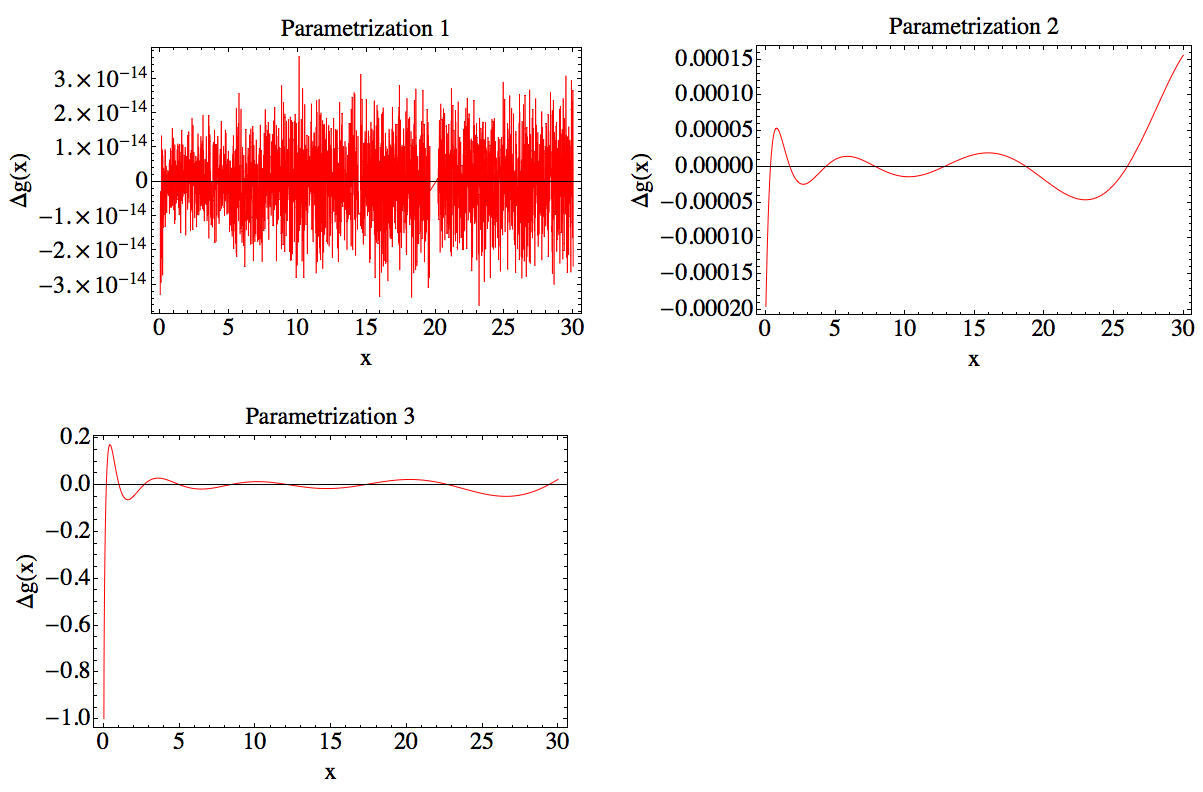
\includegraphics[width=\linewidth]{RelativeErrorPDFPolynomialCompoundPoissonExponential}
\caption{Erreur relative de l'approximation polynomiale, avec différentes paramétrisations, de la densité de probabilité d'une distribution $\left[\mathcal{P}(4),\Gamma(1,2)\right]$.}		
\label{RelativeErrorPDFPolynomialCompoundPoissonExponential}
\end{figureth}
\begin{figureth}			
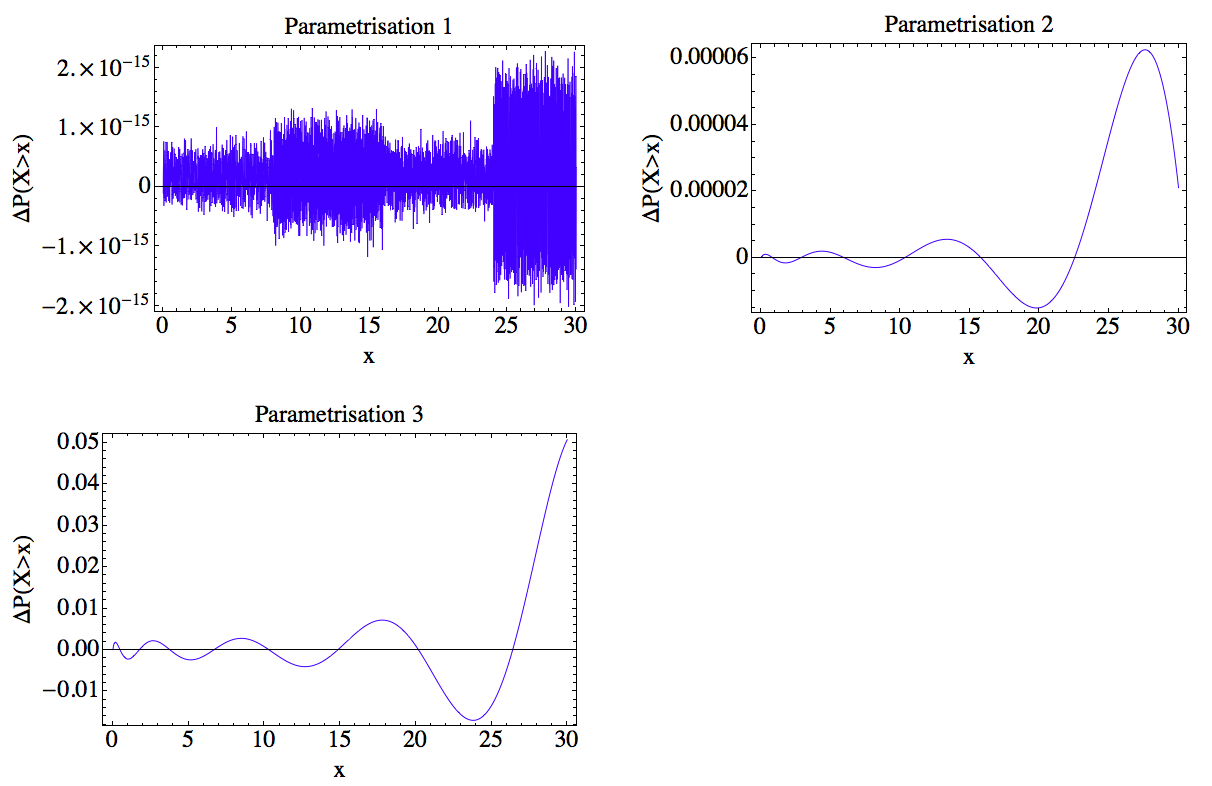
\includegraphics[width=\linewidth]{RelativeErrorSurvivalPolynomialCompoundPoissonExponentialParametrization}
\caption{Erreur relative de l'approximation polynomiale, avec différentes paramétrisations, de la \gls{fds} d'une distribution $\left[\mathcal{P}(4),\Gamma(1,2)\right]$.}		
\label{RelativeErrorSurvivalPolynomialCompoundPoissonExponentialParametrization}
	\end{figureth}

\begin{tableth}
		\caption[Approximations de la \gls{fds} d'une loi $\left(\mathcal{P}(4),\Gamma(1,4)\right)$ par la méthode d'approximation polynomiale]{\gls{fds} de la variable aléatoire $X$ de loi composée $\left[\mathcal{P}(4),\Gamma(1,1/2)\right]$ approchée par la méthode d'approximation polynomiale suivant différentes paramétrisations.}
			\label{TableSurvivalPolynomialPoissonExponential}
		\begin{tabular}{|c||c|c|c|c|c|}
\hline
$x$ &Exact &Param. $1$ & Param. $2$ & Param. $3$ \\
\hline
\hline
 3. & 0.806382 & 0.806382 & 0.806382 & 0.807966 \\
 6. & 0.573092 & 0.573092 & 0.573092 & 0.572258 \\
 9. & 0.364357 & 0.364357 & 0.364356 & 0.365284 \\
 12. & 0.21241 & 0.21241 & 0.212411 & 0.21165 \\
 15. & 0.115555 & 0.115555 & 0.115555 & 0.115619 \\
 18. & 0.0594094 & 0.0594094 & 0.0594088 & 0.0598344 \\
 21. & 0.0291366 & 0.0291366 & 0.0291363 & 0.028992 \\
 24. & 0.0137285 & 0.0137285 & 0.0137288 & 0.0134971 \\
 27. & 0.00624886 & 0.00624886 & 0.00624924 & 0.00630265 \\
 30. & 0.00275979 & 0.00275979 & 0.00275985 & 0.00289996 \\
\hline
		\end{tabular}
	\end{tableth}

\begin{tableth}
		\caption[Erreur relative ($\%$) sur la \gls{fds} d'une loi $\left(\mathcal{P}(4),\Gamma(1,2)\right)$ associée à la méthode d'approximation polynomiale]{Erreur relative en $\%$, à $10^{-5}$ près, sur la \gls{fds} de la variable aléatoire $X$ de loi composée $\left[\mathcal{P}(4),\Gamma(1,2)\right]$ approchée par la méthode polynomiale suivant différentes paramétrisations.}
			\label{TableRelativeErrorSurvivalPolynomialCompoundPoissonExponential}
		\begin{tabular}{|c||c|c|c|c|}
\hline
$x$ & Param. $1$ & Param. $2$ & Param. $3$ \\
\hline
\hline
 3. & 0. & 0.00003 & 0.19645 \\
 6. & 0. & 0. & -0.14558 \\
 9. & 0. & -0.00025 & 0.25437 \\
 12. & 0. & 0.00041 & -0.3579 \\
 15. & 0. & 0.0003 & 0.05592 \\
 18. & 0. & -0.00105 & 0.71535 \\
 21. & 0. & -0.00124 & -0.49631 \\
 24. & 0. & 0.00203 & -1.6853 \\
 27. & 0. & 0.00607 & 0.8607 \\
 30. & 0. & 0.0021 & 5.07896 \\
\hline
		\end{tabular}
	\end{tableth}

La paramétrisation $1$ permet une approximation nettement meilleure que les deux autres paramétrisations. La paramétrisation $2$ est associée à des niveaux d\rq{}erreur acceptables qui semblent constants en fonction de $x$. Les résultats pour la paramétrisation $3$ ne sont pas désastreux mais l'erreur semble augmenter avec $x$. En effet, le niveau d'erreur atteint $5\%$ lorsque $x=30$. Dans ce cas de figure, le respect du Corollaire \ref{CorrolaryParameterChoiceUnivariate} est indispensable pour obtenir de bons résultats comme le prouvent les erreurs obtenues avec les paramétrisations $1$ et $2$. La Figure \ref{RelativeErrorPDFPolynomialCompoundPoissonExponential} révèle aussi un problème en $x=0$ pour l'approximation de la densité avec la paramétrisation $3$. L'autre enseignement est qu'une bonne approximation passe par une mesure de référence proche de la mesure de probabilité gouvernant le montant des sinistres plutôt que proche de la mesure de probabilité de la distribution composée. Cette conclusion est interessante car contre-intuitive. La méthode d'approximation polynomiale est parfois assimilée à une approximation paramétrique réajustée par un développement polynomial. Dans ce cas, il semblerait logique que la mesure de référence soit aussi proche que possible de la densité inconnue. Dans la cas de la distribution composée $\left[\mathcal{P}(\lambda),\Gamma(1,\beta)\right]$, l'expression de la densité \eqref{DefectiveDensityCompoundPoissonExponential} est très proche de la formule d'approximation polynomiale \eqref{PolynomialApproximationG} avec la paramétrisation $1$.\\ 

Ces remarques conduisent à opter pour la paramétrisation $1$ pour comparer l\rq{}approximation polynomiale aux autres méthodes. La Figure \ref{RelativeErrorSurvivalDifferentMethodCompoundPoissonExponential} représente l\rq{}erreur relative sur la \gls{fds} de la distribution composée $\left[\mathcal{P}(4),\Gamma(1,2)\right]$ avec l\rq{}approximation polynomiale, l\rq{}approximation basée sur l\rq{}inversion de la transformée de Fourier, la méthode des moments exponentiels et l\rq{}algorithme de Panjer. Le Tableau \ref{TableRelativeErrorSurvivalDifferentMethodCompoundPoissonExponential} donne les valeurs numériques de ces erreurs relatives pour certaines valeurs de $x$. Le Tableau \ref{TableSurvivalDifferentMethodCompoundPoissonExponential} donne les valeurs numériques de la \gls{fds} obtenues via les différentes méthodes numériques.\\
\begin{figureth}
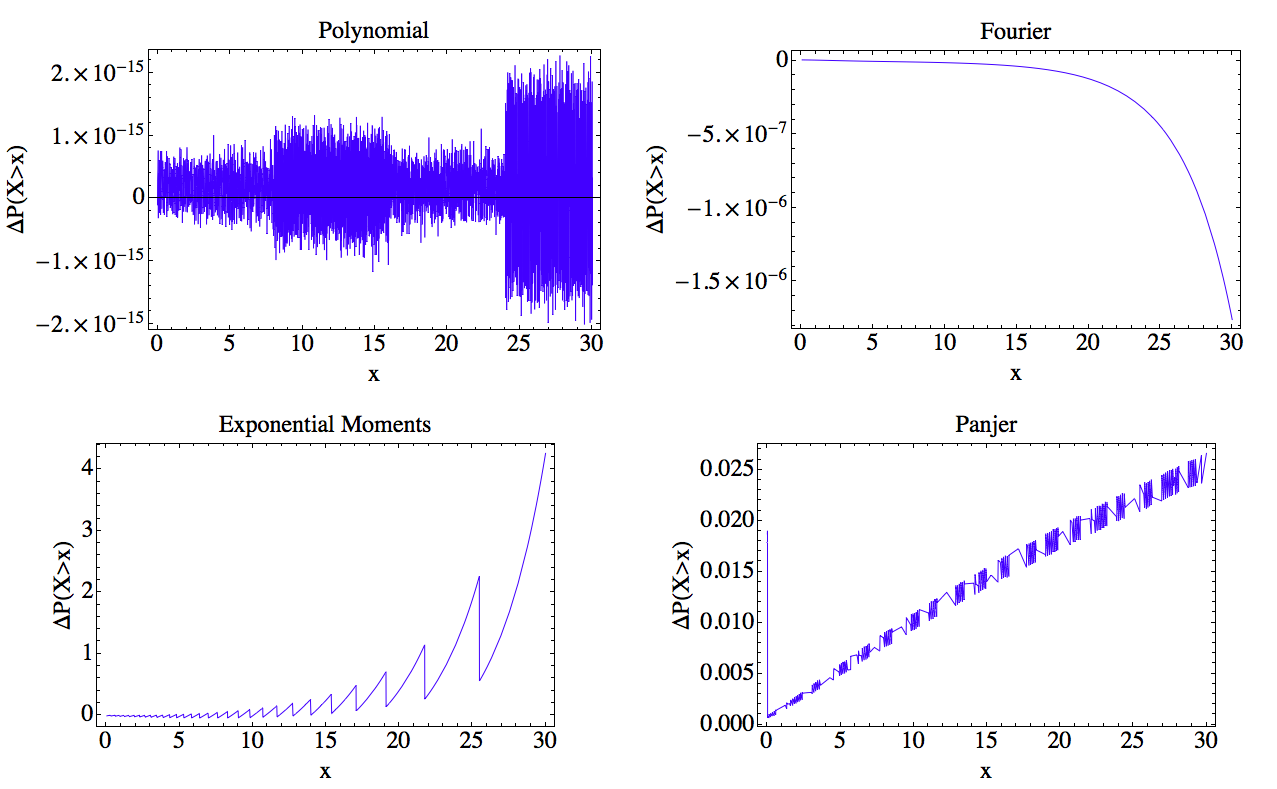
\includegraphics[width=\linewidth]{RelativeErrorSurvivalDifferentMethodCompoundPoissonExponential}
\caption{Erreur relative de l'approximation polynomiale de la \gls{fds} d'une distribution  $\left[\mathcal{P}(4),\Gamma(1,1/2)\right]$ avec différentes méthodes.}		
\label{RelativeErrorSurvivalDifferentMethodCompoundPoissonExponential}
\end{figureth}
\begin{tableth}
		\caption[Approximations de la \gls{fds} d'une loi $\left(\mathcal{P}(4),\Gamma(1,2)\right)$]{\gls{fds} de la variable aléatoire $X$ de loi composée $\left[\mathcal{P}(4),\Gamma(1,2)\right]$ approchée par différentes méthodes.}
			\label{TableSurvivalDifferentMethodCompoundPoissonExponential}
		\begin{tabular}{|c||c|c|c|c|c|}
\hline
$x$ & Exact&Polynomial & Fourier & Exponential Moment &Panjer \\
\hline
\hline
 3. & 0.806382 & 0.806382 & 0.806382 & 0.805233 & 0.808772 \\
 6. & 0.573092 & 0.573092 & 0.573092 & 0.560555 & 0.576346 \\
 9. & 0.364357 & 0.364357 & 0.364357 & 0.390845 & 0.367403 \\
 12. & 0.21241 & 0.21241 & 0.21241 & 0.220259 & 0.214731 \\
 15. & 0.115555 & 0.115555 & 0.115555 & 0.14352 & 0.117098 \\
 18. & 0.0594094 & 0.0594094 & 0.0594094 & 0.0785728 & 0.0603396 \\
 21. & 0.0291366 & 0.0291366 & 0.0291366 & 0.0521104 & 0.0296565 \\
 24. & 0.0137285 & 0.0137285 & 0.0137285 & 0.0305607 & 0.014002 \\
 27. & 0.00624886 & 0.00624886 & 0.00624886 & 0.0145444 & 0.00638581 \\
 30. & 0.00275979 & 0.00275979 & 0.00275979 & 0.0145444 & 0.00282554 \\
\hline
		\end{tabular}
	\end{tableth}

\begin{tableth}
		\caption[Erreur relative ($\%$) sur la \gls{fds} d'une loi $\left(\mathcal{P}(4),\Gamma(1,2)\right)$]{Erreur relative en $\%$, à $10^{-5}$ près, sur la \gls{fds} de la variable aléatoire $X$ de loi composée $\left[\mathcal{P}(4),\Gamma(1,2)\right]$, approchée par différentes méthodes.}
			\label{TableRelativeErrorSurvivalDifferentMethodCompoundPoissonExponential}
		\begin{tabular}{|c||c|c|c|c|}
\hline
$x$ & Polynomial & Fourier & Exponential Moment &Panjer \\
\hline
\hline
3. & 0. & 0. & -0.14243 & 0.29637 \\
 6. & 0. & 0. & -2.18774 & 0.56776 \\
 9. & 0. & 0. & 7.26981 & 0.83609 \\
 12. & 0. & 0. & 3.69503 & 1.09255 \\
 15. & 0. & 0. & 24.2007 & 1.33558 \\
 18. & 0. & -0.00001 & 32.2566 & 1.56579 \\
 21. & 0. & -0.00002 & 78.8485 & 1.78436 \\
 24. & 0. & -0.00003 & 122.608 & 1.99258 \\
 27. & 0. & -0.00008 & 132.753 & 2.19157 \\
 30. & 0. & -0.00018 & 427.012 & 2.38237 \\
\hline
		\end{tabular}
	\end{tableth}

L\rq{} approximation polynomiale est bien meilleure que ses concurentes dans ce cas. L\rq{}inversion de la transformée de Fourier arrive en deuxième position avec de très bonnes performances également. L\rq{}algorithme de Panjer donne des résultats acceptables, l'erreur relative semble augmenter linéairement avec $x$. La méthode des moments exponentiels ferme la marche, l\rq{}erreur explose litteralement pour $x\geq21$.\\ 

La Figure \ref{PDFSurvivalStopLossPolynomialCompoundPoissonExponential} représente la densité, la \gls{fds}, la \gls{fdr} et la prime \textit{stop-loss} associées à la variable aléatoire $X$ résultant de l\rq{}approximation polynomiale avec la paramétrisation $1$ et un ordre de troncature $K=30$. Le Tableau \ref{TableStopLossPolynomialCompoundPoissonExponential} donne les valeurs numériques de la prime \textit{stop-loss} usuelle calculées via l\rq{}approximation polynomiale et la méthode de Monte Carlo ainsi que l\rq{}écart relatif entre les deux.\\
\begin{figureth}
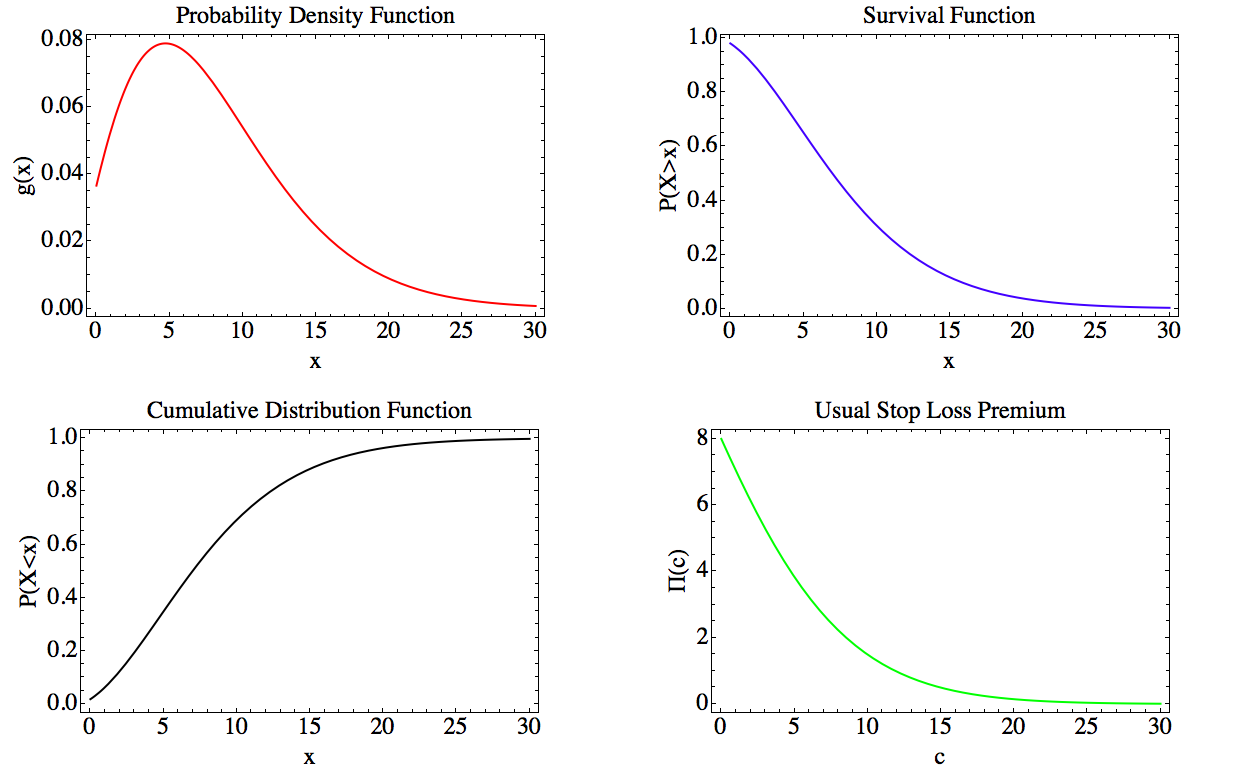
\includegraphics[width=\linewidth]{PDFSurvivalStopLossPolynomialCompoundPoissonExponential}
\caption{Approximation polynomiale de la densité défaillante, de la \gls{fds}, de la \gls{fdr} et de la prime \textit{stop-loss} usuelle pour une distribution $\left[\mathcal{P}(4),\Gamma(1,2)\right]$.}		
\label{PDFSurvivalStopLossPolynomialCompoundPoissonExponential}
\end{figureth}
	\begin{tableth}
		\caption[Calcul de la prime \textit{stop-loss} pour une loi $\left(\mathcal{P}(4),\Gamma(1,1/2)\right)$]{Evaluation de la prime \textit{stop-loss} usuelle pour une loi composée $\left[\mathcal{P}(4),\Gamma(1,1/2)\right]$ via l'approximation polynomiale et  des simulations de Monte-Carlo.}
			\label{TableStopLossPolynomialCompoundPoissonExponential}
		\begin{tabular}{|c||c|c|c|c|}
\hline
$c$ & Monte-Carlo & Polynomial & Relative Error $(\%)$ \\
\hline
\hline
 3. & 5.27937 & 5.28977 & 0.19704 \\
 6. & 3.21013 & 3.2187 & 0.26682 \\
 9. & 1.81787 & 1.82481 & 0.38157 \\
 12. & 0.969839 & 0.974639 & 0.49493 \\
 15. & 0.49123 & 0.494874 & 0.74191 \\
 18. & 0.237786 & 0.240618 & 1.1907 \\
 21. & 0.110721 & 0.112688 & 1.77607 \\
 24. & 0.0498302 & 0.0510734 & 2.49487 \\
 27. & 0.0217394 & 0.0224882 & 3.44426 \\
 30. & 0.00939161 & 0.00965032 & 2.75466 \\
\hline
		\end{tabular}
	\end{tableth}

Cette illustration est importante car elle montre une utilisation très pratique de l\rq{}approximation polynomiale de la \gls{fds}. L\rq{}approximation polynomiale est manipulable, il est possible de l\rq{}intégrer pour approcher d\rq{}autres quantités avec une bonne précision. Sur cet exemple, les primes \textit{stop loss} issues de l\rq{}approximation polynomiale prennent des valeurs numériques proches des valeurs obtenues par Monte-Carlo. Le calcul de la prime \textit{stop-loss} $\Pi_{1,c}(X)$, par Monte-Carlo, pour différentes valeurs de $c$ nécessite la manipulation et la sauvegarde de jeux de données contenant $10^{6}$ observations. Ce processus est coûteux en temps de calcul et en mémoire. Une visualisation graphique à l\rq{}image de celle de la Figure \ref{PDFSurvivalStopLossPolynomialCompoundPoissonExponential} serait obtenue en interpolant les valeurs calculées pour différentes valeurs de $c$. L\rq{}utilisation de l\rq{}approximation polynomiale consiste à ré-injecter l\rq{}approximation de la fonction de survie dans l\rq{}expression intégrale \eqref{StopLossPremiumIntegral} de la prime \textit{stop-loss}. Le résultat du calcul intégral est une approximation de $\Pi_{1,c}(X)$ valable pour toute valeur de $c$. 
\subsection{Le cas des sinistres de loi gamma $\Gamma(\alpha,\beta)$}
Les montants de sinistre sont modélisés par une suite $\{U_{i}\}_{i\in\mathbb{N}}$ de variable aléatoires \gls{iid} suivant une loi gamma $\Gamma(\alpha,\beta)$. Dans ce cas, la densité et la \gls{fds} de la variable aléatoire $X$ ne sont pas disponibles explicitement. Une approximation de la densité défaillante est obtenue en tronquant simplement la série infinie
\begin{equation*}
g_{X}(x)=\sum_{l=0}^{+\infty}\frac{e^{-\lambda}}{\lambda^{l}{l!}}\times\frac{e^{-x/\beta}x^{l\times\alpha-1}}{\beta^{l\times\alpha}\Gamma(l\times\alpha)},
\end{equation*}
à l'ordre $L$. Cette approximation est particulièrement efficace pour $\lambda$ faible eu égard à la décroisssance rapide des probabilités de la loi de Poisson. Ce proxy va servir de référence pour apprécier les performances des méthodes d'approximations.\\

La \gls{fgm} de $X$ de loi de probabilité composée $\left[\mathcal{P}(\lambda),\Gamma(\alpha,\beta)\right]$ est donnée par 
\begin{equation}\label{fgmCompoundPoissonGamma}
\mathcal{L}_{X}(s)=\exp\left[\lambda\left(\frac{1}{1-s\beta}\right)^{\alpha}-1\right],
\end{equation}
ce qui implique que $\gamma_{X}=\frac{1}{\beta}$. La fonction génératrice des coefficients est obtenue par réinjection de la \gls{fgm} \eqref{fgmCompoundPoissonGamma} dans \eqref{GeneratingFunctionTomgf}, avec
\begin{equation}\label{CoeficientGeneratingFunctionCompoundPoissonExponential}
\mathcal{C}(z)=(1+z)^{-r}\exp\left\{\lambda\left[\frac{m^{\alpha}(1+z)^{\alpha}-\left[m+z(m-\beta)\right]^{\alpha}}{\left[m+z(m-\beta)\right]^{\alpha}}\right]\right\}.
\end{equation}
La paramétrisation
\begin{equation}\label{CompoundPoissonGammaParametrization1}
m_{1}=\beta\hspace{0.1cm};\hspace{0.1cm}r_{1}=1,
\end{equation}
simplifie la fonction génératrice des coefficients, avec 
\begin{equation*}
\mathcal{C}(z)=(1+z)^{-1}\exp\left[\lambda(1+z)^{\alpha}\right].
\end{equation*}
La paramétrisation \eqref{CompoundPoissonGammaParametrization1} est conforme au Corollaire \ref{CorrolaryParameterChoiceUnivariate}. La paramétrisation $2$, définie par
\begin{equation}\label{CompoundPoissonGammaParametrization2}
m_{2}=\beta\hspace{0.1cm};\hspace{0.1cm}r_{2}=\alpha,
\end{equation}
simplifie la fonction génératrice des coefficients, avec 
\begin{equation*}
\mathcal{C}(z)=(1+z)^{-\alpha}\exp\left[\lambda(1+z)^{\alpha}\right].
\end{equation*}
La paramétrisation \eqref{CompoundPoissonGammaParametrization2} n\rq{}est pas conforme au Corollaire \ref{CorrolaryParameterChoiceUnivariate}. L\rq{}idée est de rapprocher autant que possible la mesure de référence de la mesure de probabilité du montant des sinistres. La paramétrisation $1$ fait correspondre le moment d\rq{}ordre 1 et la paramétrisation $2$ fait correspondre les moments d\rq{}ordre $1$ et $2$. Pour l\rq{}illustration numérique, le paramètre de loi de Poisson est $\lambda=2$ et les paramètres de la loi gamma sont $\alpha=3$ et $\beta=1$. La paramétrisation $3$ est définie par l\rq{}équation \eqref{ParametrizationDeMerde2}, ce qui donne 
\begin{equation}\label{CompoundPoissonGammaParametrization3}
m_{3}=6\hspace{0.1cm};\hspace{0.1cm}r_{3}=1,
\end{equation}
après applications numériques. La paramétrisation $4$ est définie par l\rq{}équation \eqref{ParametrizationDeMerde1}, ce qui donne 
\begin{equation}\label{CompoundPoissonGammaParametrization4}
m_{4}=5\hspace{0.1cm};\hspace{0.1cm}r_{4}=\frac{6}{5},
\end{equation}
après applications numériques. La paramétrisation \eqref{CompoundPoissonGammaParametrization3} est conforme au Corollaire \ref{CorrolaryParameterChoiceUnivariate}, ce n\rq{}est pas le cas de la paramétrisation \eqref{CompoundPoissonGammaParametrization4}. L\rq{}ordre de troncature est $K=85$ pour chacune des quatres paramétrisations. La Figure \ref{RelativeErrorPDFPolynomialCompoundPoissonGamma} représente l\rq{}erreur relative de l\rq{}approximation polynomiale sur la densité défaillante $g_{X}(x)$, d\rq{}une loi de probabilité composée $\left[\mathcal{P}(2),\Gamma(3,1)\right]$, associée aux différentes paramétrisations, en fonction des valeurs de $x$. La Figure \ref{RelativeErrorSurvivalDifferentParametrizationCompoundPoissonGamma} représente l\rq{}erreur relative de l\rq{}approximation polynomiale sur la \gls{fds} $\overline{F_{X}}(x)$, d\rq{}une loi de probabilité composée $\left[\mathcal{P}(2),\Gamma(3,1)\right]$, associée aux différentes paramétrisations, en fonction des valeurs de $x$. Le Tableau \ref{TableSurvivalPolynomialCompoundPoissonGamma} donne les valeurs approchées grâce à la méthode d\rq{}approximation polynomiale suivant les différentes paramétrisations. La Tableau \ref{TableRelativeErrorSurvivalPolynomialCompoundPoissonGamma} donne les valeurs numériques des erreurs relatives liées à l\rq{}emploi de l\rq{}approximation polynomiale suivant les différentes paramétrisations.\\
\begin{figureth}			
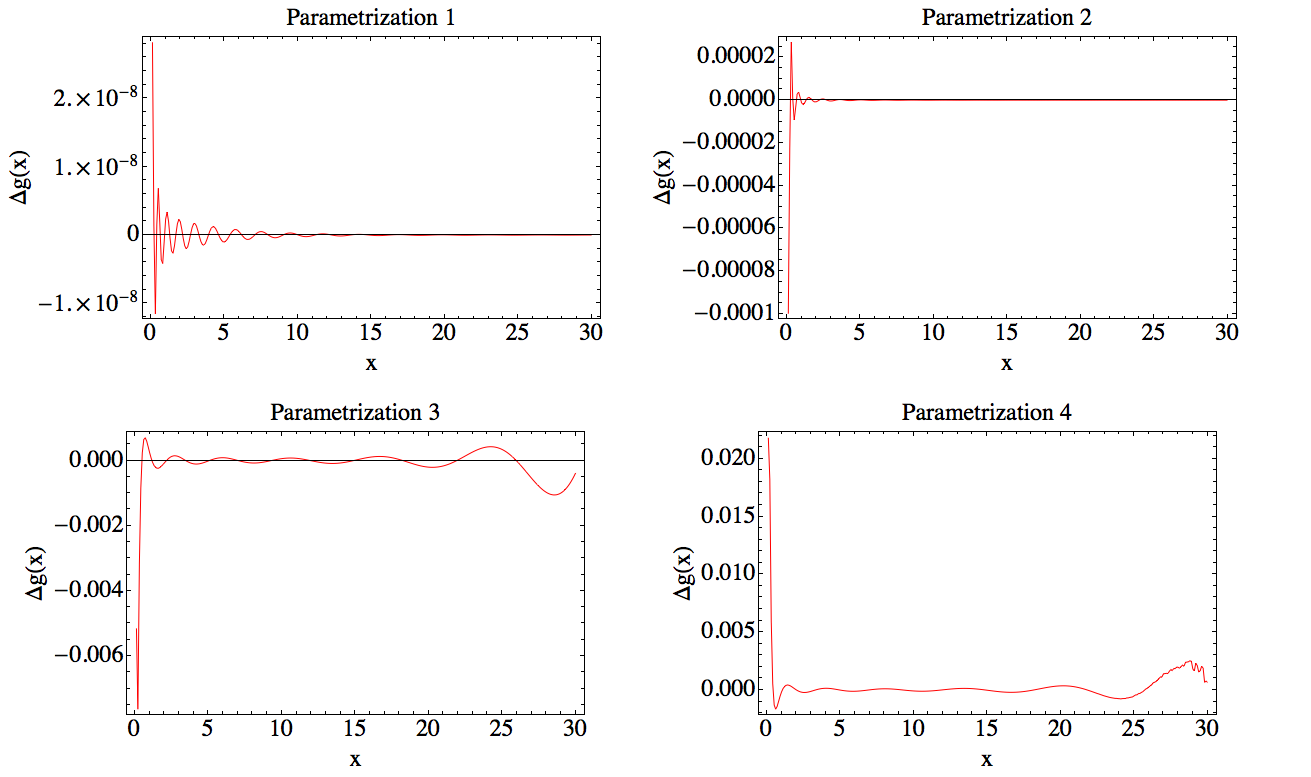
\includegraphics[width=\linewidth]{RelativeErrorPDFPolynomialCompoundPoissonGamma}
\caption{Erreur relative de l'approximation polynomiale, avec différentes paramétrisations, de la densité de probabilité d'une distribution $\left[\mathcal{P}(2),\Gamma(3,1)\right]$.}		
\label{RelativeErrorPDFPolynomialCompoundPoissonGamma}
\end{figureth}
\begin{figureth}			
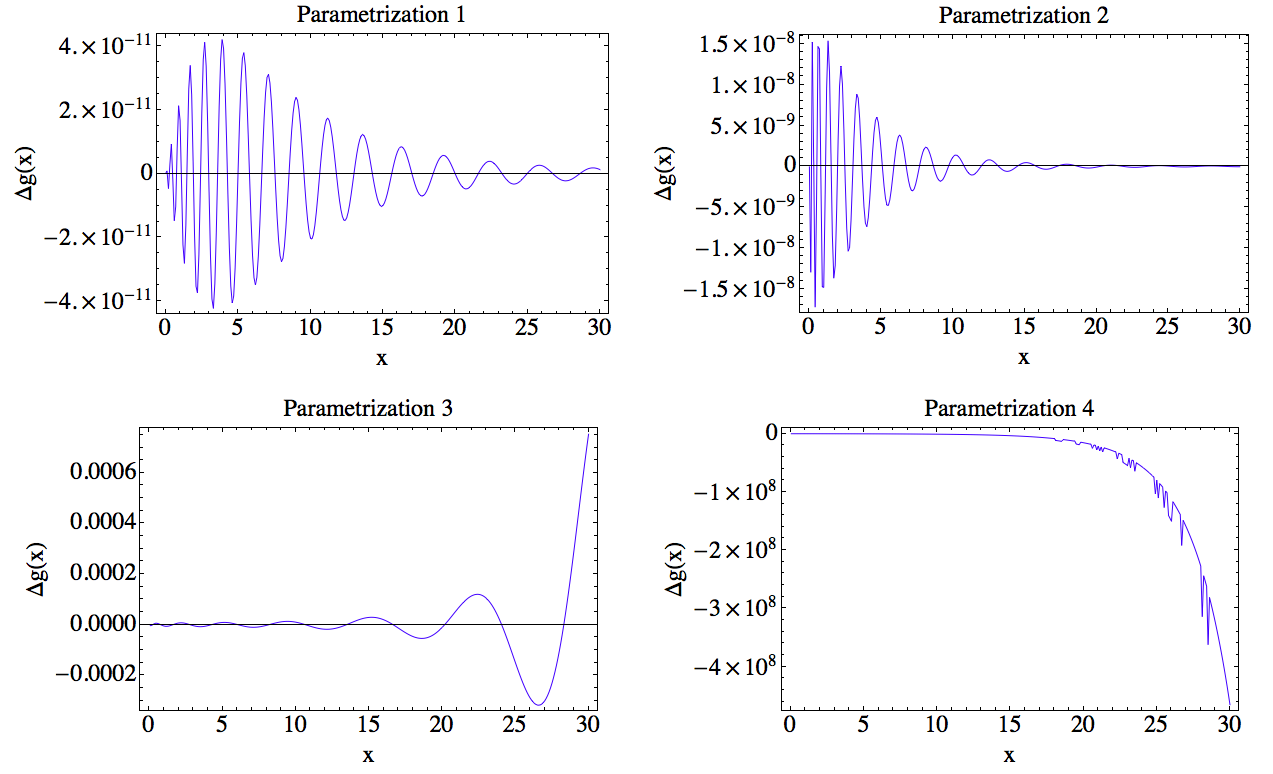
\includegraphics[width=\linewidth]{RelativeErrorSurvivalDifferentParametrizationCompoundPoissonGamma}
\caption{Erreur relative de l'approximation polynomiale, avec différentes paramétrisations, de la \gls{fds} d'une distribution $\left[\mathcal{P}(2),\Gamma(3,1)\right]$.}		
\label{RelativeErrorSurvivalDifferentParametrizationCompoundPoissonGamma}
	\end{figureth}

\begin{tableth}
		\caption[Approximations polynomiales de la \gls{fds} d'une loi $\left(\mathcal{P}(2),\Gamma(3,1)\right)$]{Evaluation de la \gls{fds} de la variable aléatoire $X$ de loi composée $\left[\mathcal{P}(2),\Gamma(3,1)\right]$ via l'approximation polynomiale avec différentes paramétrisations.}
			\label{TableSurvivalPolynomialCompoundPoissonGamma}
		\begin{tabular}{|c||c|c|c|c|c|}
\hline
$x$ & Exact&Param. $1$  &Param. $2$&Param. $3$&Param. $4$ \\
\hline
\hline
3. & 0.685132 & 0.685132 & 0.685132 & 0.685129684 & -196608. \\
 6. & 0.4313 & 0.4313 & 0.4313 & 0.4312998 & -196608. \\
 9. & 0.238763 & 0.238763 & 0.238763 & 0.2387659551 & -196608. \\
 12. & 0.118895 & 0.118895 & 0.118895 & 0.11889306 & -196608. \\
 15. & 0.0542376 & 0.0542376 & 0.0542376 & 0.0542391 & -196608. \\
 18. & 0.0229767 & 0.0229767 & 0.0229767 & 0.0229756268 & -196608. \\
 21. & 0.00913388 & 0.00913388 & 0.00913388 & 0.00913441 & -196608. \\
 24. & 0.00343513 & 0.00343513 & 0.00343513 & 0.0034351619 & -196608. \\
 27. & 0.00123021 & 0.00123021 & 0.00123021 & 0.00122984 & -196608. \\
 30. & 0.000421752 & 0.000421752 & 0.000421752 & 0.000422070029 & -196608. \\

\hline
		\end{tabular}
	\end{tableth}

\begin{tableth}
		\caption[Erreur relative ($\%$) sur la \gls{fds} d'une loi $\left(\mathcal{P}(2),\Gamma(3,1)\right)$ associée à la méthode d'approximation polynomiale]{Erreur relative en $\%$, à $10^{-5}$ près, sur la \gls{fds} de la variable aléatoire $X$ de loi composée $\left[\mathcal{P}(2),\Gamma(3,1)\right]$ approchée par méthode polynomiale suivant différentes paramétrisations.}
			\label{TableRelativeErrorSurvivalPolynomialCompoundPoissonGamma}
		\begin{tabular}{|c||c|c|c|c|}
\hline
$x$ & Param. $1$ & Param. $2$ & Param. $3$& Param. $4$ \\
\hline
\hline
3. & 0. & 0. & -0.0004 & $\infty$ \\
 6. & 0. & 0. & 0.00006 & $\infty$ \\
 9. & 0. & 0. & 0.00111 & $\infty$ \\
 12. & 0. & 0. & -0.00181 & $\infty$ \\
 15. & 0. & 0. & 0.00287 & $\infty$ \\
 18. & 0. & 0. & -0.00469 & $\infty$ \\
 21. & 0. & 0. & 0.00586 & $\infty$ \\
 24. & 0. & 0. & 0.0008 & $\infty$ \\
 27. & 0. & 0. & -0.03009 & $\infty$ \\
 30. & 0. & 0. & 0.07546 & $\infty$ \\
\hline
		\end{tabular}
	\end{tableth}

L\rq{}erreur relative explose pour la paramétrisation $4$. La paramétrisation \eqref{CompoundPoissonGammaParametrization2} bien que non conforme au Corollaire \ref{CorrolaryParameterChoiceUnivariate} est celle qui fonctionne le mieux, tallonée par la paramétrisation \eqref{CompoundPoissonGammaParametrization1}. Cela montre que le Corollaire \ref{CorrolaryParameterChoiceUnivariate} est une condition suffisante pour que l\rq{}approximation polynomiale \eqref{PDFPolynomialApproximationNumerical} soit valide, cette condition n\rq{}est cependant pas nécessaire. Ce cas particulier montre aussi que plus la mesure de référence est proche de la mesure de probabilité des montants de sinistres, plus la méthode d\rq{}approximation est performante. La comparaison avec les autres méthodes d\rq{}approximation est effectuée avec la paramétrisation $1$. La Figure \ref{RelativeErrorSurvivalDifferentMethodCompoundPoissonGamma} représente l\rq{}erreur relative sur la \gls{fds} de la loi composée $\left[\mathcal{P}(2),\Gamma(3,1)\right]$ suivant la méthode numérique utilisée. Le Tableau \ref{TableSurvivalPolynomialCompoundPoissonGammaDifferentMethod} donne les valeurs numériques de la \gls{fds} résultant de l\rq{}emploi des différentes méthodes. Le Tableau \ref{TableRelativeErrorSurvivalPolynomialCompoundPoissonGammaDifferentMethod} donne les valeurs numériques de l\rq{}erreur relative sur la \gls{fds} suite à l\rq{}approximation via les différentes méthodes.\\

\begin{figureth}			
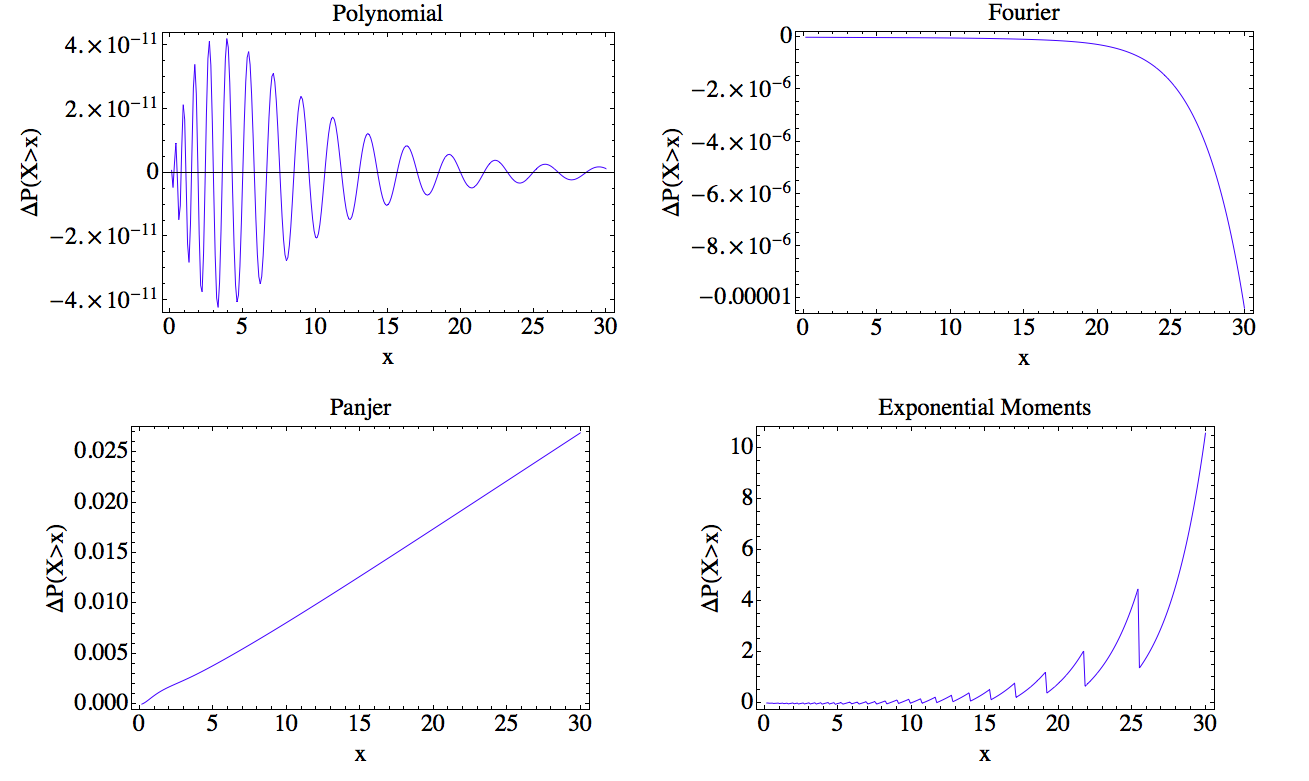
\includegraphics[width=\linewidth]{RelativeErrorSurvivalDifferentMethodCompoundPoissonGamma}
\caption{Erreur relative de l\rq{}approximation polynomiale de la \gls{fds} d'une distribution $\left[\mathcal{P}(2),\Gamma(3,1)\right]$ suivant différentes méthodes numériques.}		
\label{RelativeErrorSurvivalDifferentMethodCompoundPoissonGamma}
	\end{figureth}
\begin{tableth}
		\caption[Approximations de la \gls{fds} d'une loi $\left(\mathcal{P}(2),\Gamma(3,1)\right)$ via différentes méthodes]{Evaluation de la \gls{fds} de la variable aléatoire $X$ de loi composée $\left[\mathcal{P}(2),\Gamma(3,1)\right]$ par différentes méthodes.}
			\label{TableSurvivalPolynomialCompoundPoissonGammaDifferentMethod}
		\begin{tabular}{|c||c|c|c|c|c|}
\hline
$x$ &Exact& Polynomial&Fourier  & Exponential Moment &Panjer \\
\hline
\hline
3. & 0.685132 & 0.685132 & 0.685132 & 0.685203 & 0.686771 \\
 6. & 0.4313 & 0.4313 & 0.4313 & 0.422254 & 0.433313 \\
 9. & 0.238763 & 0.238763 & 0.238763 & 0.266124 & 0.24049 \\
 12. & 0.118895 & 0.118895 & 0.118895 & 0.129356 & 0.120076 \\
 15. & 0.0542376 & 0.0542376 & 0.0542376 & 0.076121 & 0.0549268 \\
 18. & 0.0229767 & 0.0229767 & 0.0229767 & 0.0364145 & 0.0233334 \\
 21. & 0.00913388 & 0.00913388 & 0.00913387 & 0.0222035 & 0.00930159 \\
 24. & 0.00343513 & 0.00343513 & 0.00343513 & 0.011718 & 0.003508 \\
 27. & 0.00123021 & 0.00123021 & 0.00123021 & 0.00489717 & 0.00125982 \\
 30. & 0.000421752 & 0.000421752 & 0.000421747 & 0.00489717 & 0.000433105 \\
\hline
		\end{tabular}
	\end{tableth}

	\begin{tableth}
		\caption[Erreur relative ($\%$) liée à l\rq{}approximation de la \gls{fds} d'une loi $\left(\mathcal{P}(2),\Gamma(3,1)\right)$]{Erreur relative en $\%$, à $10^{-5}$ près, sur la \gls{fds} de la variable aléatoire $X$ de loi composée $\left[\mathcal{P}(2),\Gamma(3,1)\right]$ via différentes méthodes.}
			\label{TableRelativeErrorSurvivalPolynomialCompoundPoissonGammaDifferentMethod}
		\begin{tabular}{|c||c|c|c|c|}
\hline
$x$ & Polynomial&Fourier & Exponential Moment &Panjer \\
\hline
\hline
3. & 0. & 0. & 0.01036 & 0.2392 \\
 6. & 0. & 0. & -2.0972 & 0.46687 \\
 9. & 0. & 0. & 11.4594 & 0.72337 \\
 12. & 0. & 0. & 8.79806 & 0.99333 \\
 15. & 0. & -0.00001 & 40.3474 & 1.27079 \\
 18. & 0. & -0.00001 & 58.4844 & 1.55239 \\
 21. & 0. & -0.00004 & 143.089 & 1.83622 \\
 24. & 0. & -0.00012 & 241.122 & 2.12116 \\
 27. & 0. & -0.00036 & 298.076 & 2.40651 \\
 30. & 0. & -0.00104 & 1061.15 & 2.69184 \\
\hline
		\end{tabular}
	\end{tableth}
Le classement en termes de performance est le même que dans le cas où les montants de sinistres sont distribués exponentiellement. La méthode polynomiale arrive en tête, suivie de la méthode d\rq{}inversion de la transformée de Fourier, l\rq{}algorithme de Panjer puis pour finir la méthode des moments exponentiels. La Figure \ref{PDFSurvivalStopLossPolynomialCompoundPoissonGamma} propose une visualisation graphique de l\rq{}approximation polynomiale, obtenue en utilisant la paramétrisation $1$ et un ordre de troncature $K=85$, de la densité de probabilité, de la \gls{fds}, de la \gls{fdr}, et de la prime \textit{stop-loss} usuelle de la loi composée $\left[\mathcal{P}(2),\Gamma(3,1)\right]$. Le Tableau \ref{TableStopLossPolynomialCompoundPoissonGamma} donne les valeurs numériques de la prime \textit{stop-loss} usuelle calculées par la méthode polynomiale et la méthode de Monte-Carlo. 
\begin{figureth}
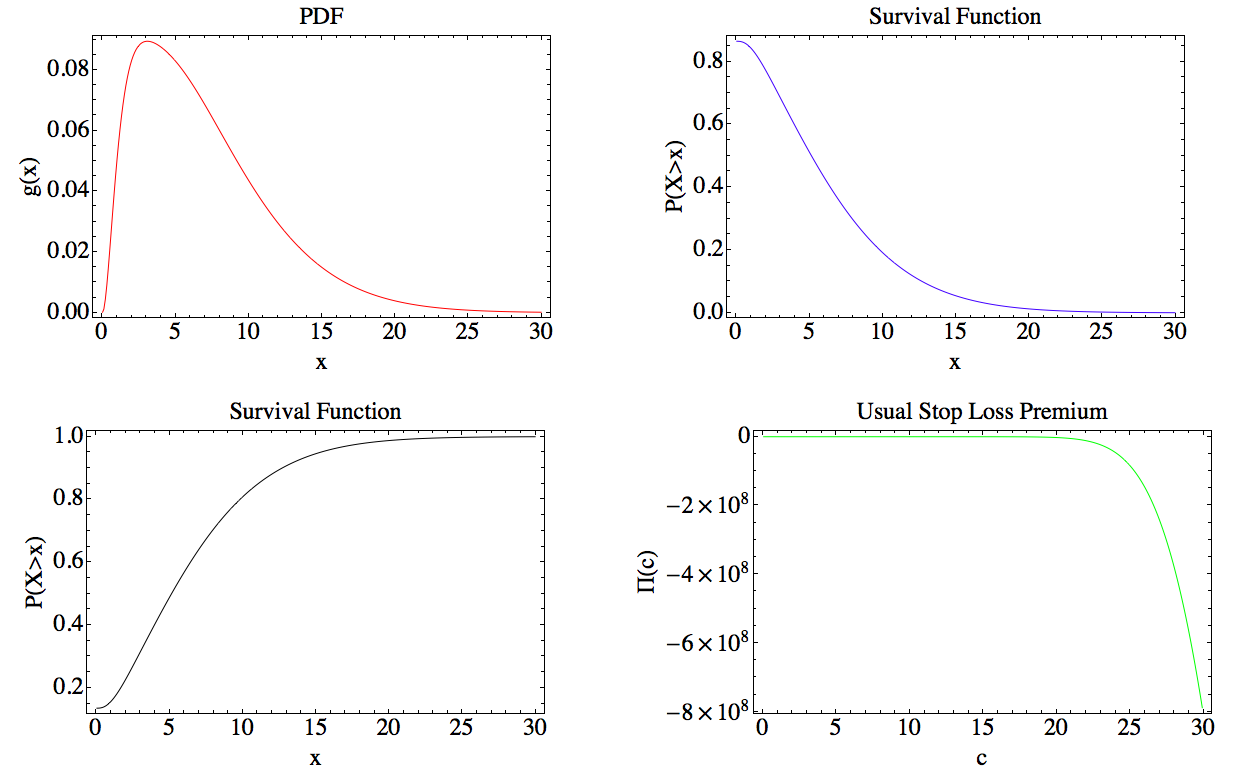
\includegraphics[width=\linewidth]{PDFSurvivalStopLossPolynomialCompoundPoissonGamma}
\caption{Approximation polynomiale de la densité défaillante, de la \gls{fds}, de la \gls{fdr} et de la prime \textit{stop-loss} usuelle pour une distribution $\left[\mathcal{P}(2),\Gamma(3,1)\right]$.}		
\label{PDFSurvivalStopLossPolynomialCompoundPoissonGamma}
\end{figureth}

	\begin{tableth}
		\caption[Calcul de la prime \textit{stop-loss} pour une loi $\left(\mathcal{P}(2),\Gamma(3,1)\right)$]{Evaluation de la prime \textit{stop-loss} usuelle pour une loi composée $\left[\mathcal{P}(2),\Gamma(3,1)\right]$ via l'approximation polynomiale et des simulations de Monte-Carlo.}
			\label{TableStopLossPolynomialCompoundPoissonGamma}
		\begin{tabular}{|c||c|c|c|c|}
\hline
$c$ & Monte-Carlo & Polynomial & Relative Error $(\%)$ \\
\hline
\hline
0 & 5.99316 & 6. & 0.114172 \\
 3 & 3.59554 & 3.60192 & 0.177357 \\
 6 & 1.93243 & 1.9526 & 1.04382 \\
 9 & 0.94746 & 29.3862 & 3001.58 \\
 12 & 0.429122 & 834.273 & 194314. \\
 15 & 0.181003 & -14846.1 & $\infty$\\
 18 & 0.0716428 & -415589. & $\infty$\\
 21 & 0.0269423 &$\infty$ & $\infty$\\
 24 & 0.00976161 & $\infty$ & $\infty$\\
 27 & 0.00342669 & $\infty$ & $\infty$\\
 30 & 0.00113488 & $\infty$ & $\infty$\\
\hline
		\end{tabular}
	\end{tableth}
La prime \textit{stop-loss} explose pour un seuil de rétention $c\geq9$, ce qui est assez surprenant au vu des bons résultats obtenus dans l\rq{}approximation de la densité de probabilité, de la \gls{fds}, et de la \gls{fdr}. L\rq{}emploi d\rq{}un ordre de troncature trop grand entraine des problèmes numériques lors de l\rq{}évaluation de l\rq{}intégrale \eqref{StopLossPolynomialApproximationNumerical}. Il n\rq{}y a aucune raison pour que l\rq{}intégration en elle-même engendre une telle erreur. Cette erreur est sûrement due à des erreurs d\rq{}arrondi et à une maladresse dans la façon d\rq{}évaluer numériquement les intégrales via Mathematica. Ces problèmes seront à résoudre dans les suites de ce travail.     

\subsection{Le cas des sinistres de loi uniforme $\mathcal{U}\left[\alpha,\beta\right]$}
Le montant des sinistres est modélisé par une suite $\{U_{i}\}_{i\in\mathbb{N}}$ de variables aléatoires \gls{iid} suivant une loi uniforme $\mathcal{U}(\alpha,\beta)$. 
\begin{Def}
Soit $X$ une variable aléatoire de loi uniforme $\mathcal{U}(\alpha,\beta)$, avec $\alpha,\beta\in\mathbb{R}$ et $\alpha<\beta$. La densité de $X$ est donnée par 
\begin{equation}\label{DensityUniform}
f_{X}(x)=\frac{1}{\beta-\alpha},\hspace{0.2cm}x\in[\alpha,\beta],
\end{equation}
et sa \gls{fgm} par 
\begin{equation}\label{fgmPhaseType}
\mathcal{L}_{X}(s)=\frac{e^{s\beta}-e^{s\alpha}}{\beta-\alpha}.
\end{equation}
\end{Def}
Dans ce cas, la densité et la \gls{fds} de la variable aléatoire $X$ ne sont pas disponibles explicitement, la méthode d\rq{}inversion numérique de la transformée de Fourier est utilisée pour mesurer la précision des méthodes numériques sur la \gls{fds} de la variable aléatoire $X$. La \gls{fgm} de $X$ de loi composée $\left[\mathcal{P}(\lambda),\mathcal{U}(\alpha,\beta)\right]$ est donnée par 
\begin{equation}\label{fgmCompoundPoissonUniform}
\mathcal{L}_{X}(s)=\exp\left\{\lambda\left[\frac{e^{s\beta}-e^{s\alpha}}{(\beta-\alpha)s}-1\right]\right\},
\end{equation}
ce qui implique que $\gamma_{X}=+\infty$. La fonction génératrice des coefficients admet une forme qui ne permet pas la prise de décision en ce qui concerne la paramétrisation. Au vu des résultats obtenus sur les deux exemples précédents, il est logique d\rq{}opter pour des paramétrisations basées sur les moments de la distribution de probabilité du montant des sinistres. La paramétrisation $1$, définie par 
\begin{equation}\label{CompoundPoissonUniformParametrization1}
m_{1}=\frac{\mathbb{V}(U)}{\mathbb{E}(U)}=\frac{(\beta-\alpha)^{2}}{6(\alpha+\beta)}\hspace{0.1cm};\hspace{0.1cm}r_{1}=\frac{\mathbb{E}(U)^{2}}{\mathbb{V}(U)}=\frac{3(\alpha+\beta)^{2}}{(\beta-\alpha)^{2}},
\end{equation}
fait coïncider les moments d\rq{}ordre $1$ et $2$ de la mesure de référence avec ceux de la distribution du montant des sinistres. La paramétrisation $2$, définie par
\begin{equation*}\label{CompoundPoissonUniformParametrization2}
m_{2}=\mathbb{E}(U)=\frac{(\beta-\alpha)}{2}\hspace{0.1cm};\hspace{0.1cm}r_{2}=1
\end{equation*}
fait coïncider le moment d\rq{}ordre $1$ de la mesure de référence avec celui de la distribution du montant des sinistres. Pour l\rq{}illustration, le paramètre de la loi de Poisson est $\lambda=3$ et les paramètres de la loi uniforme $\mathcal{U}(\alpha,\beta)$ sont $\alpha=0$ et $\beta=10$. Ce qui donne 
\begin{equation}\label{CompoundPoissonUniformParametrization1}
m_{1}=\frac{5}{3}\hspace{0.1cm};\hspace{0.1cm}r_{1}=3,
\end{equation}
et 
\begin{equation}\label{CompoundPoissonUniformParametrization1}
m_{2}=5\hspace{0.1cm};\hspace{0.1cm}r_{2}=1,
\end{equation}
après applications numériques. La paramétrisation $3$ est définie par l\rq{}équation \eqref{ParametrizationDeMerde2}, ce qui donne 
\begin{equation}\label{CompoundPoissonUniformParametrization3}
m_{3}=15\hspace{0.1cm};\hspace{0.1cm}r_{3}=1,
\end{equation}
après applications numériques. La paramétrisation $4$ est définie par l\rq{}équation \eqref{ParametrizationDeMerde1}, ce qui donne 
\begin{equation}\label{CompoundPoissonGammaParametrization4}
m_{4}=\frac{23}{3}\hspace{0.1cm};\hspace{0.1cm}r_{4}=\frac{45}{23},
\end{equation}
après applications numériques. Les paramétrisations $2$ et $3$ sont conformes au Corollaire \ref{CorrolaryParameterChoiceUnivariate}, ce n\rq{}est pas le cas des paramétrisations $1$ et $4$. L\rq{}ordre de troncature est $K=75$ pour chacune des paramétrisations étudiées. La Figure \ref{RelativeErrorSurvivalDifferentParametrizationCompoundPoissonUniform} montre l\rq{}ecart relatif de l\rq{}approximation polynomiale de la \gls{fds} par rapport à l\rq{}approximation issue de l\rq{}inversion de la transformée de Fourier, suivant la paramétrisation. Le Tableau \ref{TableSurvivalDifferentParametrizationCompoundPoissonUniform} donne les valeurs numériques de la \gls{fds} approchée par la méthode d\rq{}inversion numérique de la transformée de Fourier et la méthode polynomiale. Le Tableau \ref{TableRelativeErrorSurvivalDifferentParametrizationCompoundPoissonUniform} donne les valeurs numériques des écarts entre les approximations polynomiales et celles renvoyées par l\rq{}inversion numérique de la transformée de Fourier. \\
\begin{figureth}			
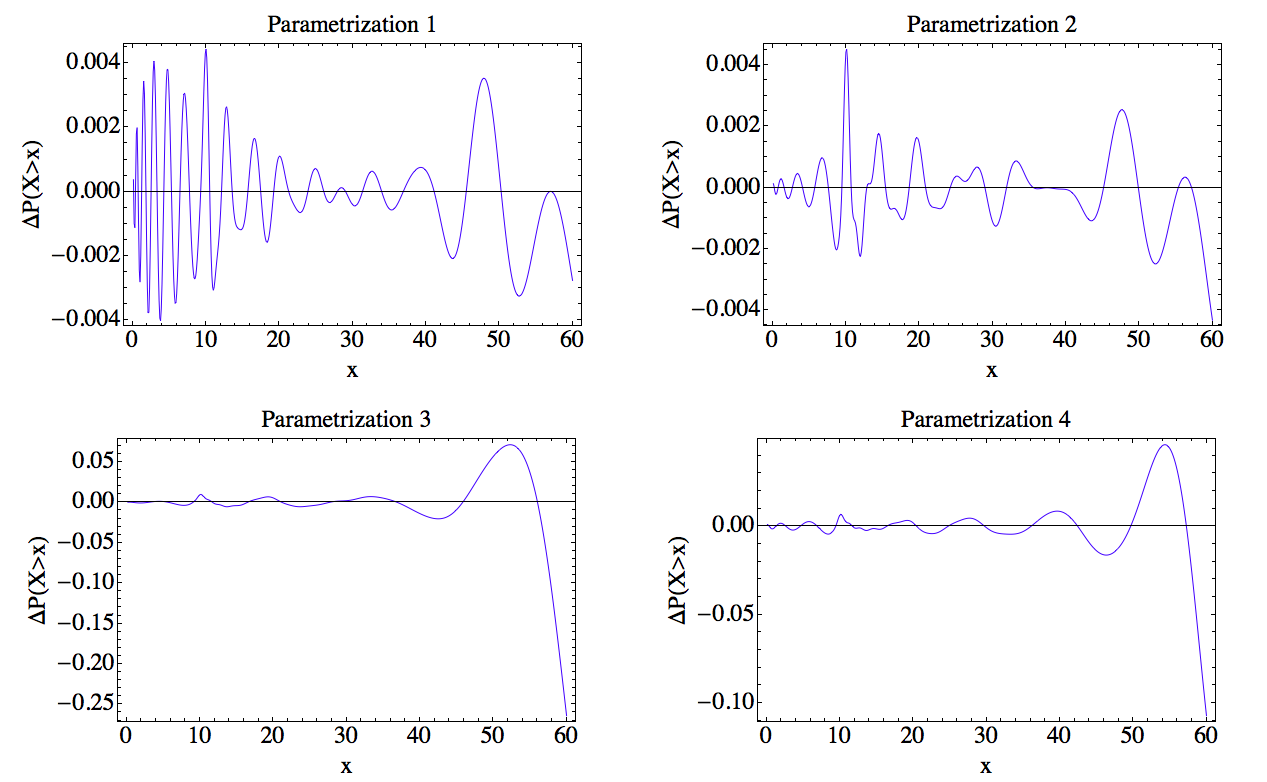
\includegraphics[width=\linewidth]{RelativeErrorSurvivalDifferentParametrizationCompoundPoissonUniform}
\caption{Erreur relative de l'approximation polynomiale, avec différentes paramétrisations, de la \gls{fds} d'une distribution $\left[\mathcal{P}(3),\mathcal{U}(0,10)\right]$ par rapport à méthode d\rq{}inversion numérique de la transformée de Fourier.}		
\label{RelativeErrorSurvivalDifferentParametrizationCompoundPoissonUniform}
\end{figureth}
\begin{tableth}
		\caption[Approximations polynomiales de la \gls{fds} d'une loi $\left(\mathcal{P}(4),\mathcal{U}(0,10)\right)$]{Evaluation de la \gls{fds} de la variable aléatoire $X$ de loi composée $\left[\mathcal{P}(4),\mathcal{U}(0,10)\right]$ via la méthode d'approximation polynomiale avec différentes paramétrisations.}
			\label{TableSurvivalDifferentParametrizationCompoundPoissonUniform}
		\begin{tabular}{|c||c|c|c|c|c|}
\hline
$x$ & Fourier&Param. $1$ & Param. $2$ &Param. $3$ &Param. $4$ \\
\hline
\hline
  6. & 0.811227 & 0.80865 & 0.811507 & 0.810796205 & 0.81332372 \\
 12. & 0.56834 & 0.568012 & 0.567072 & 0.56746466 & 0.5678477 \\
 18. & 0.34191 & 0.341455 & 0.341587 & 0.3434973 & 0.3426809 \\
 24. & 0.17857 & 0.178591 & 0.178539 & 0.177635 & 0.1782032 \\
 30. & 0.081776 & 0.0817428 & 0.0816851 & 0.081952935 & 0.0817116 \\
 36. & 0.033478 & 0.0334635 & 0.0334768 & 0.033576449 & 0.03347229796\\
 42. & 0.0124404 & 0.0124292 & 0.0124332 & 0.012192117 & 0.01247017 \\
 48. & 0.00420535 & 0.00422016 & 0.00421571 & 0.0043344158 & 0.0041541479 \\
 54. & 0.00132527 & 0.00132197 & 0.00132356 & 0.0014034753 & 0.00138585 \\
 60. & 0.000386308 & 0.000385234 & 0.000384629 & 0.00028410264& 0.0003448 \\


\hline
		\end{tabular}
	\end{tableth}
	\begin{tableth}
		\caption[Erreur relative ($\%$) sur la \gls{fds} d'une loi $\left(\mathcal{P}(4),\mathcal{U}(0,10)\right)$ associée à la méthode d'approximation polynomiale]{Erreur relative en $\%$, à $10^{-5}$ près, sur la \gls{fds} de la variable aléatoire $X$ de loi composée $\left[\mathcal{P}(4),\mathcal{U}(0,10)\right]$ via la méthode d'approximation polynomiale avec différentes paramétrisations.}
			\label{TableRelativeErrorSurvivalDifferentParametrizationCompoundPoissonUniform}
		\begin{tabular}{|c||c|c|c|c|}
\hline
$x$ & Param. $1$ & Param. $2$ &Param. $3$ &Param. $4$ \\
\hline
\hline
 6. & -0.31771 & 0.03449 & -0.05311 & 0.25845 \\
 12. & -0.05772 & -0.2231 & -0.15394 & -0.08653 \\
 18. & -0.13288 & -0.09454 & 0.4643 & 0.22553 \\
 24. & 0.01139 & -0.01759 & -0.52331 & -0.2055 \\
 30. & -0.04068 & -0.11119 & 0.21631 & -0.07873 \\
 36. & -0.04315 & -0.00353 & 0.29409 & -0.01701 \\
 42. & -0.0902 & -0.05834 & -1.99604 & 0.23904 \\
 48. & 0.35227 & 0.24625 & 3.06909 & -1.21755 \\
 54. & -0.24908 & -0.1292 & 5.90079 & 4.57148 \\
 60. & -0.27808 & -0.43455 & -26.457 & -10.7411 \\
\hline
		\end{tabular}
	\end{tableth}

Les écarts pour les paramétrisations $3$ et $4$ sont très importants. Les deux autres paramétrisations renvoient des valeurs proches de celles obtenues via l\rq{}inversion numérique de la transformée de Fourier, notamment la paramétrisation $2$. Si il est admis que la méthode d\rq{}inversion de la transformée de Fourier est aussi précise que dans les cas d\rq{}étude précédent, alors le niveau d\rq{}erreur de l\rq{}approximation polynomiale est bien plus important que dans les cas précédent. Ce constat s\rq{}explique par le fait que la loi uniforme est bien plus éloignée de la mesure de référence que la loi gamma. L\rq{}augmentation de l\rq{}ordre de troncature devrait pouvoir résoudre ce problème, il pourrait cependant s\rq{}accompagner de difficultés d\rq{}ordre numérique. La paramétrisation $2$ est retenue pour effectuer la comparaison avec les autres méthodes numériques. La Figure \ref{RelativeErrorSurvivalDifferentMethodCompoundPoissonUniform} permet la visualisation des écarts entre l\rq{}approximation de la \gls{fds} de $X$ via l\rq{}inversion de la transformée de Fourier et les autres méthodes numériques. Le Tableau \ref{TableSurvivalDifferentMethodCompoundPoissonUniform} donne les valeurs numériques de la \gls{fds} approchée par les différentes méthodes. Le Tableau \ref{TableRelativeErrorSurvivalDifferentMethodCompoundPoissonUniform} donne les valeurs numériques des écarts entre l\rq{}approximation de la \gls{fds} via l\rq{}inversion de la transformée de Fourier et les autres méthodes numériques. 
\begin{figureth}			
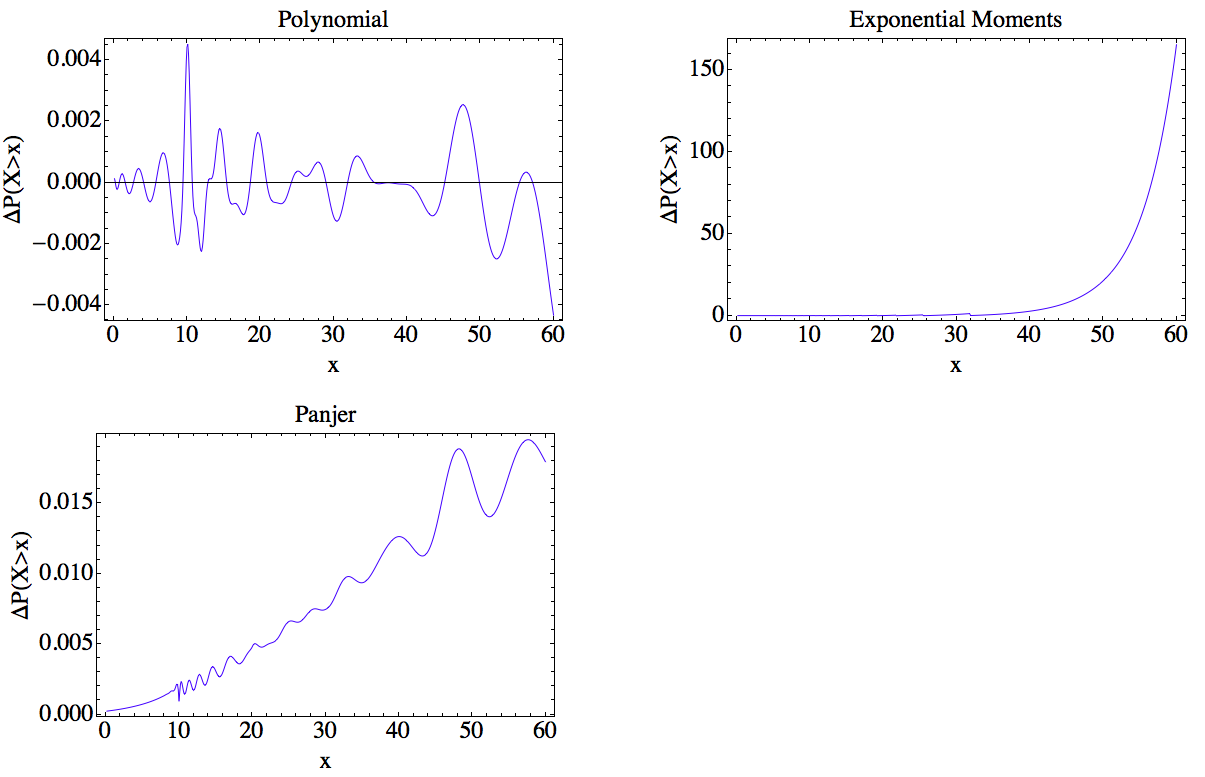
\includegraphics[width=\linewidth]{RelativeErrorSurvivalDifferentMethodCompoundPoissonUniform}
\caption{Erreur relative, en $\%$, sur la \gls{fds} d'une distribution $\left[\mathcal{P}(2),\mathcal{U}(0,10)\right]$ suivant la méthode numérique utilisée.}		
\label{RelativeErrorSurvivalDifferentMethodCompoundPoissonUniform}
	\end{figureth}

	\begin{tableth}
		\caption[Approximations de la \gls{fds} d'une loi $\left(\mathcal{P}(4),\mathcal{U}(0,10)\right)$]{Evaluation de la \gls{fds} de la variable aléatoire $X$ de loi composée $\left[\mathcal{P}(4),\mathcal{U}(0,10)\right]$ par différentes méthodes.}
			\label{TableSurvivalDifferentMethodCompoundPoissonUniform}
		\begin{tabular}{|c||c|c|c|c|c|}
\hline
$x$ & Fourier&Polynomial  & Exponential Moment &Panjer \\
\hline
\hline
6 & 0.811227 & 0.811507 & 0.798633 & 0.811957 \\
 12 & 0.56834 & 0.567072 & 0.557872 & 0.569321 \\
 18 & 0.34191 & 0.341587 & 0.35222 & 0.343157 \\
 24 & 0.17857 & 0.178539 & 0.216235 & 0.179621 \\
 30 & 0.081776 & 0.0816851 & 0.140781 & 0.0823872 \\
 36 & 0.033478 & 0.0334768 & 0.0644221 & 0.0338055 \\
 42 & 0.0124404 & 0.0124332 & 0.0644221 & 0.0125867 \\
 48 & 0.00420535 & 0.00421571 & 0.0644221 & 0.00428459 \\
 54 & 0.00132527 & 0.00132356 & 0.0644221 & 0.00134572 \\
 60 & 0.000386308 & 0.000384629 & 0.0644221 & 0.000393232 \\

\hline
		\end{tabular}
	\end{tableth}

	\begin{tableth}
		\caption[Erreur relative ($\%$) sur la \gls{fds} d'une loi $\left(\mathcal{P}(4),\mathcal{U}(0,10)\right)$]{Erreur relative en $\%$, à $10^{-5}$ près, sur la \gls{fds} de la variable aléatoire $X$ de loi composée $\left[\mathcal{P}(4),\mathcal{U}(0,10)\right]$ par rapport à la méthode d'inversion de la transformée de Fourier.}
			\label{TableRelativeErrorSurvivalDifferentMethodCompoundPoissonUniform}
		\begin{tabular}{|c||c|c|c|c|}
\hline
$x$ & Polynomial & Exponential Moment &Panjer \\
\hline
\hline
  6 & 0.03449 & -1.55242 & 0.08995 \\
 12 & -0.2231 & -1.84175 & 0.17261 \\
 18 & -0.09454 & 3.01549 & 0.36475 \\
 24 & -0.01759 & 21.0926 & 0.58869 \\
 30 & -0.11119 & 72.1542 & 0.74738 \\
 36 & -0.00353 & 92.4311 & 0.97826 \\
 42 & -0.05834 & 417.844 & 1.17585 \\
 48 & 0.24625 & 1431.91 & 1.88423 \\
 54 & -0.1292 & 4761.04 & 1.543 \\
 60 & -0.43455 & 16576.4 & 1.79229 \\
\hline
		\end{tabular}
	\end{tableth}
Dans ce cas particulier, l\rq{}algorithme propose une approximation concurrentielle avec la méthode polynomiale. La méthode des moments exponentiels performe nettement moins bien que les deux autres méthodes. La Figure \ref{PDFSurvivalStopLossPolynomialCompoundPoissonUniform} montre l\rq{}approximation polynomiale de la densité, de la \gls{fds}, de la \gls{fdr}, et de la prime \textit{stop-loss} usuelle, obtenues avec la paramétrisation $2$ et un ordre de troncature $K=75$. Le Tableau \ref{TableStopLossPolynomialCompoundPoissonUniform} donne les valeurs numériques des approximations par la méthode polynomiale et la méthode de Monte-Carlo de la prime \textit{stop-loss} usuelle ainsi que l\rq{}écart relatif entre les deux.\\
\begin{figureth}
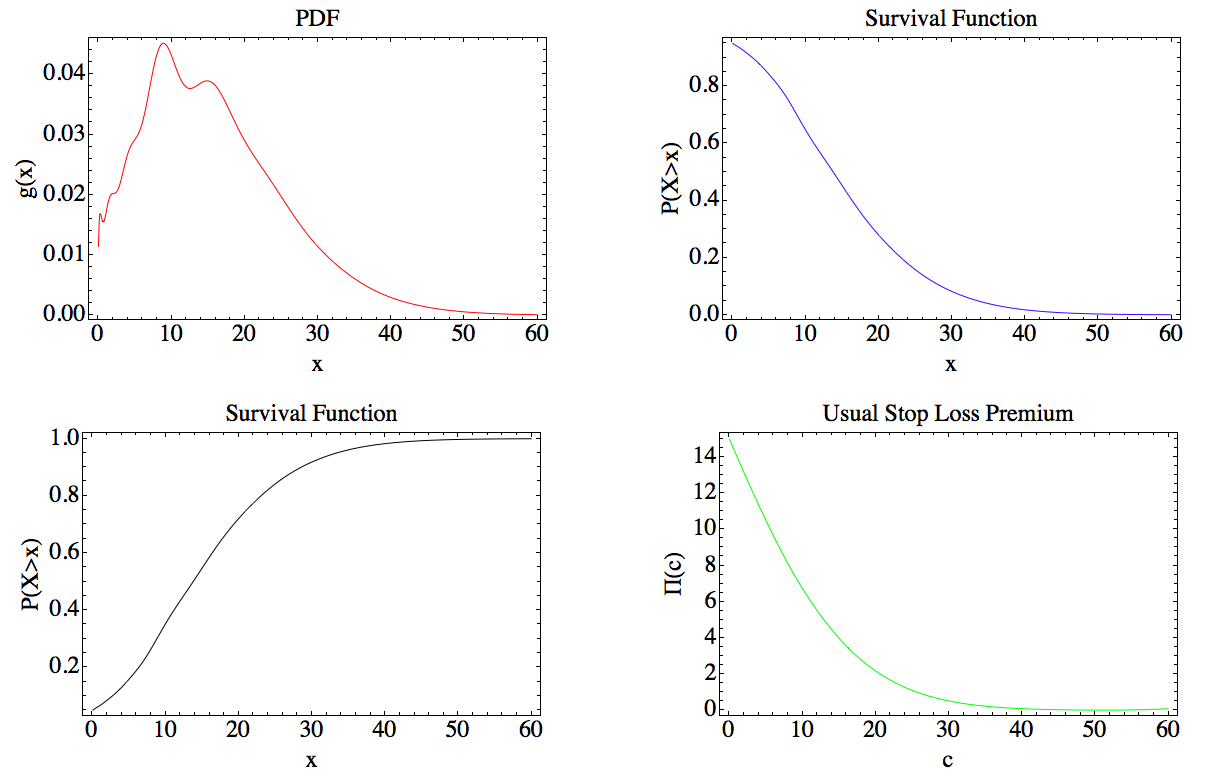
\includegraphics[width=\linewidth]{PDFSurvivalStopLossPolynomialCompoundPoissonUniform}
\caption{Approximation polynomiale de la densité défaillante, de la \gls{fds}, de la \gls{fdr} et de la prime \textit{stop-loss} usuelle pour une distribution $\left[\mathcal{P}(3),\mathcal{U}(0,10)\right]$.}		
\label{PDFSurvivalStopLossPolynomialCompoundPoissonUniform}
\end{figureth}

	\begin{tableth}
		\caption[Calcul de la prime \textit{stop-loss} pour une loi $\left(\mathcal{P}(4),\mathcal{U}(0,10)\right)$]{Evaluation de la prime \textit{stop-loss} usuelle pour une loi composée $\left[\mathcal{P}(4),\mathcal{U}(0,10)\right]$ via l'approximation polynomiale et des simulations de Monte-Carlo.}
			\label{TableStopLossPolynomialCompoundPoissonUniform}
		\begin{tabular}{|c||c|c|c|c|}
\hline
$c$ & Monte-Carlo & Polynomial & Relative Error $(\%)$\\
\hline
\hline
0 & 5.99316 & 6. & 0.114172 \\
 3 & 3.59554 & 3.60192 & 0.177357 \\
 6 & 1.93243 & 1.9526 & 1.04382 \\
 9 & 0.94746 & 29.3862 & 3001.58 \\
 12 & 0.429122 & 834.273 & 194314. \\
 15 & 0.181003 & $\infty$ & $\infty$ \\
 18 & 0.0716428 & $\infty$ & $\infty$ \\
 21 & 0.0269423 & $\infty$ & $\infty$ \\
 24 & 0.00976161 & $\infty$ & $\infty$ \\
 27 & 0.00342669 & $\infty$ & $\infty$ \\
 30 & 0.00113488 & $\infty$ & $\infty$ \\
\hline
		\end{tabular}
	\end{tableth}

La méthode d\rq{}approximation polynomiale se heurte comme dans le cas d\rq{}étude précédent à des difficultés d\rq{}ordre numérique dans l\rq{}approximation de la prime \textit{stop-loss} usuelle pour des valeurs de seuils de rétention élevé $c\geq9$.\\

La méthode d\rq{}approximation polynomiale est une méthode efficace, qui concurrence l\rq{}inversion numérique de la transformée de Fourier dans certains cas. La restriction sur le choix des paramètres conformément au Corollaire \ref{CorrolaryParameterChoiceUnivariate} assure la validité de l\rq{}approximation et l\rq{}obtention de résultats au moins comparables à l\rq{}algorithme de Panjer. Son avantage réside dans l\rq{}exploitation directe de l\rq{}approximation de la densité pour l\rq{}évaluation de la \gls{fds} et de la prime \textit{stop-loss}. Les difficultés numériques doivent pouvoir être contournées en prêtant soin à l\rq{}implémentation de la méthode polynomiale. Les temps de calcul sont aussi un frein pour obtenir l\rq{}approximation de la \gls{fds} pour un ordre de troncature supérieur à $100$. Encore une fois, une implémentation plus adroite doit permettre de diminuer les temps de calcul. Le principal avantage de la méthode polynomiale réside dans la perspective d\rq{}une application statistique lorsque des données sont disponibles.     

%\subsection{Application à la distribution binomiale négative composée}
%\subsubsection{Le cas des sinistres de loi gamma $\Gamma(\alpha,\beta)$}
%
%
%
%
%\subsubsection{Le cas des sinistres de loi uniforme $\mathcal{U}\left[\alpha,\beta\right]$}

\section{Perspectives en statistique}
\subsection{Estimation de la densité de probabilité via la représentation polynomiale}\label{Chapter2Section3}
Soit $X_{1},\ldots,X_{n}$ un échantillon \gls{iid}, de taille $n$, issu de la loi de probabilité $\mathbb{P}_{X}$. Un estimateur de la densité est obtenu à partir de l'approximation \eqref{PolynomialApproximationf}, avec 
\begin{equation}\label{PolynomialEstimator}
\widehat{f_{X}}^{K}(x)=\widehat{f_{X,\nu}}^{K}(x)\widehat{f_{\nu}}(x).
\end{equation}
L'écriture $\widehat{f_{\nu}}$ sous-entend une estimation statistique des paramètres de la mesure de probabilité de référence. La distribution de référence représente une distribution a priori. Un ordre de troncature $K=0$ équivaut à faire l'hypothèse d'un modèle paramètrique basé sur les \gls{fenq}. Le choix d'un ordre de troncature supérieur à $0$ permet d'ajuster et de corriger l'erreur de modèle via un développement polynomial. L'estimateur \eqref{PolynomialEstimator} est semi-paramétrique. La technique d'estimation du paramètre dépend du choix de la mesure de référence et du problème étudié. Afin de conserver un caractère général pour l'instant, il est supposé que les paramètres de la mesure de référence ont été estimés. Le système de polynômes $\{Q_{k}\}_{k\in\mathbb{N}}$ forme un système orthonormal par rapport à la mesure de probabilité caractérisée par la densité $\widehat{f_{\nu}}$. Cette idée de démarrer avec une première estimation paramétrique et d\rq{}ajuster à l\rq{}aide d'une projection sur une base de fonctions orthogonales remonte aux travaux de \citet{Wh58} et \citet{Br78}. Le terme \textit{prior distribution} est d\rq{}ailleurs employé pour parler de la mesure associée à $f_{\nu}$. Les travaux plus récents de \citet{Bu92} et de \citet{PrJi12} décrivent une méthode basée sur des polynômes orthogonaux par rapport à une mesure de référence, appelée fonction de poids. La méthode présentée dans \citet{PrJi12} est d'ailleurs basée sur l'approximation de la densité par les moments de la distribution qui fait l'objet de l'article \citet{Pr05} déjà cité. Dans le papier de \citet{HjGl95}, la densité par rapport à une mesure de probabilité paramétrique de référence est estimée via un estimateur à noyau.\\

L'estimateur de  $f_{X,\nu}^{K}$ est donné par 
\begin{equation}\label{Estimatorg}
\widehat{f_{X,\nu}}^{K}(x)=\sum_{k=1}^{K}\widehat{a_{k}}Q_{k}(x),
\end{equation}
où les composantes du vecteur $\widehat{\bold{a}}=(\widehat{a_{1}},\ldots,\widehat{a_{K}})$ sont estimées par 
\begin{equation}\label{EstimatorCoefficient}
\widehat{a_{k}}=w_{k}\frac{1}{n}\sum_{i=1}^{n}Q_{k}(X_{i}), \hspace{0.2cm}\forall k\in\{1,\ldots,K\}.
\end{equation}
Le vecteur $\bold{w}=(w_{1},\ldots,w_{K})$ est un modulateur dont les composantes vérifient $0\leq w_{k}\leq1$ pour $k=1,\ldots,K$. Le nombre de paramètres à estimer ne peut excéder le nombre d\rq{}observations, ce qui revient à imposer la condition $K\leq n$. Le problème d\rq{}estimation est non-paramétrique au sens où le nombre de paramètres à estimer augmente avec le nombre d\rq{}observations. L\rq{}estimation non-paramétrique de la densité via les séries othogonales est un sujet classique dans la litterature statistique. Les avantages sont, entre autres, la facilité de l'implémentation et l\rq{}efficacité en dimension supérieure à $1$. L\rq{}estimateur \eqref{Estimatorg} est original car il fait intervenir une mesure de probabilité de référence. Les estimateurs non-paramétriques de la densité de ce type sont plus souvent définis comme des développements sur des bases de fonctions orthogonales. Ces estimateurs ont été initialement introduit dans les travaux de \citet{Ce62}. Les estimateurs basés sur les fonctions de Hermite, définies comme le produit de la densité de la loi normale et des polynômes d\rq{}Hermite, ont été étudiés dans les papiers de \citet{Sc67} et \citet{Wa77}. Une extension à l\rq{}estimation de la fonction de densité et de ses dérivées est proposée dans le travail de \citet{GrPa84}. Une étude de l'estimateur basé sur les fonctions de Laguerre, définis comme le produit de la densité de la loi gamma et des polynômes de Laguerre est proposée dans le papier de \citet{Ha80}, Cet estimateur est comparé à l'estimateur basé sur les fonctions de Hermite.\\

L\rq{}optimisation du modulateur $\bold{w}$ fait l'objet de nombreux travaux. Le critère proposé dans \citet{KrTa68} revient à supposer $\bold{w}$ de la forme $(1,\ldots,1,0,\ldots,0)$. Cette idée a été reprise et affinée par exemple dans \citet{DiHa86}. Dans le travail de \citet{Wa69}, le modulateur $\bold{w}$ est optimisé pour que la suite des composantes du vecteur soit monotone, décroissante vers $0$. Le livre d\rq{}\citet{Ef99} décrit de façon exhaustive les propriétés de ces estimateurs basés sur les fonctions orthogonales, l\rq{}accent est mis sur l\rq{}utilisation des fonctions trigonométriques. Une mesure de référence, sans l\rq{}aspect paramétrique, est utilisée dans le papier de \citet{AnFi80} avec un modulateur monotone.\\

Le problème d'estimation est rapproché du \textit{Normal Mean problem} à l'image de ce qui est présenté dans les chapitres 7 et 8 de l'ouvrage de \citet{Wa06}. L'estimation des coefficients $\{\widehat{a_{k}}\}_{k\in\{1,\ldots,n\}}$ est similaire à l'estimation d'une loi gaussienne multivariée. Le vecteur aléatoire $\bold{Z}=(Z_{1},\ldots,Z_{n})$ est défini par 
\begin{equation}\label{ZDefinition}
Z_{k}=\frac{1}{n}\sum_{i=1}^{n}Q_{k}(X_{i}),\hspace{0.2cm}k=1,\ldots,n.
\end{equation}
Les composantes du vecteur $\bold{Z}$ estiment sans biais les coefficients du développement, avec
\begin{equation}
\mathbb{E}\left(Z_{k}\right)=a_{k},\hspace{0.2cm}k=1,\ldots,n.
\end{equation}
La variance de $Z_{k}$ est donnée par
\begin{equation} 
\sigma_{k,n}^{2}=\mathbb{V}(Z_{k}),\hspace{0.2cm}k=1,\ldots,n.
\end{equation}
L\rq{}\gls{eqmi} issue de l'estimation de $f_{X,\nu}$ par l'estimateur \eqref{Estimatorg} avec un ordre de troncature $K=n$ est donné par
\begin{eqnarray}
R\left(f_{X,\nu},\widehat{f_{X,\nu}}^{n} \right)&=&\mathbb{E}\left[L\left(f_{X,\nu},\widehat{f_{X,\nu}}^{n}\right)\right]\label{EqmiEstimation1}\\
&=&\sum_{k=1}^{n}(1-w_{k})^{2}a_{k}^{2}+\sum_{k=n+1}^{+\infty}a_{k}^{2}\label{SquareBias1}\\
&+&\sum_{k=1}^{n}w_{k}^{2}\sigma_{k,n}^{2}\label{Variance1}. 
\end{eqnarray} 
Le risque \eqref{EqmiEstimation1} est la somme du biais au carré \eqref{SquareBias1} et de la variance \eqref{Variance1} de l'estimateur. Le but est de trouver le modulateur $\bold{w}$ permettant d\rq{}optimiser ce risque. La quantité $\sum_{k=n+1}^{+\infty}a_{k}^{2}$ est inaccessible, elle est cependant positive et indépendante du modulateur. L'optimisation du risque \eqref{EqmiEstimation1} sur l'ensemble des modulateurs revient à optimiser
\begin{equation}\label{ModifiedRisk}
R\left(f_{X,\nu}^{n},\widehat{f_{X,\nu}}^{n} \right)=\sum_{k=1}^{n}(1-w_{k})^{2}a_{k}^{2}+\sum_{k=1}^{n}w_{k}^{2}\sigma_{k,n}^{2}.
\end{equation}
De plus, il est classique d'obtenir un résultat du type 
\begin{equation*}
a_{k}=O\left(\frac{1}{k}\right),\hspace{0.2cm}k\rightarrow+\infty.
\end{equation*}
sous des hypothèses de régularité pour la fonction $f_{X,\nu}$ et ses dérivées. La quantité $\sum_{k=n+1}^{+\infty}a_{k}^{2}$ peut alors être négligée dans un contexte d'estimation non-paramètrique de la densité dans lequel la vitesse de convergence optimale est de l'ordre de $k^{-4/5}$.\\

Dans l\rq{}expression du risque \eqref{ModifiedRisk}, interviennent des quantités inconnues qu'il est nécessaire d'estimer statistiquement. le carré des coefficients de la représentation polynomiale $a_{k}^{2}$ sont estimés sans biais, via
\begin{equation*}
\widehat{a_{k}^{2}}=Z_{k}^{2}-\sigma_{k,n}^{2},\hspace{0.2cm}k=1,\ldots,n.
\end{equation*}
Afin de garantir la positivité de l'estimation $a_{k}^{2}$ cette estimateur est modifié, avec
\begin{equation*}
\widehat{a_{k}^{2}}=\left(Z_{k}^{2}-\sigma_{k,n}^{2}\right)_{+}.
\end{equation*}
L'estimateur du risque \eqref{ModifiedRisk} à ce stade est donné par 
\begin{equation}\label{ModifiedRiskEstimator1}
\widehat{R}\left(f_{X,\nu}^{n},\widehat{f_{X,\nu}}^{n} \right)=\sum_{k=1}^{n}(1-w_{k})^{2}\left(Z_{k}^{2}-\sigma_{k,n}^{2}\right)_{+}+\sum_{k=1}^{n}w_{k}^{2}\sigma_{k,n}^{2}.
\end{equation}
\begin{Rk}
L'approche \textit{Normal Means} est justifiée par la convergence en loi du vecteur $\bold{Z}$ vers une loi gaussienne multivariée. L'application du \gls{tcl} multivarié implique que 
\begin{equation}
\sqrt{n}\left(\bold{Z}-\bold{a}\right)\underset{a.s}{\sim}\mathcal{N}\left(0,\Sigma\right),\hspace{0.2cm} n\rightarrow+\infty,
\end{equation}
où $\Sigma=\left\{Cov\left(Q_{k}(X),Q_{l}(X)\right)\right\}_{k,l\in\{1,\ldots,n\}^{2}}$ est la matrice de variance-covariance. Ce résultat peut permettre d'appliquer le théorème de Stein, voir \citet{St81}, qui donne une estimation sans biais du risque \eqref{ModifiedRisk}. Il est intéressant d'observer que l'estimation du risque de Stein, ou \gls{sure}, coïncide avec l'estimation obtenue dans l'équation \eqref{ModifiedRiskEstimator1}
\end{Rk}
Les termes de variance $\sigma_{k,n}^{2}$ sont estimés sans biais, avec 
\begin{equation}\label{VarianceEstimation}
\widehat{\sigma}_{k,n}^{2}=\frac{1}{n(n-1)}\sum_{i=1}^{n}\left[Q_{k}(X_{i})-Z_{k}\right]^{2},\hspace{0.2cm}k=1,\ldots,n.
\end{equation}
%L\rq{}application du théorème \ref{AsNormalityCoefficient} permet de proposer un estimateur du risque du type \gls{sure} par application du théorème de \citet{St81}, dont l\rq{}énoncé est le suivant:
%\begin{Theo}[Stein 1981]\label{TheoSURE}
%Soit $\bold{Z}\sim\mathcal{N}(\bold{a},\bold{V})$ un vecteur gaussien de dimension $n$, de moyenne $\bold{a}$ et de matrice de Variance-Covariance $\bold{V}=\left\{Cov\left(Z_{k},Z_{l}\right)\right\}_{k,l\in\{1,\ldots,n\}^{2}}$. Soit $\widehat{\bold{a}}=\widehat{\bold{a}}(\bold{Z})$ un estimateur de $\bold{a}$. Soit l\rq{}application $h:\mathbb{R}^{n}\mapsto\mathbb{R}^{n}$ définie par $h(\bold{Z})=\widehat{\bold{a}}-\bold{Z}$. Si $h$ est faiblement différentiable alors
%\begin{equation}\label{SUREFormula}
%\widehat{R}(\bold{Z})=\text{tr}(\bold{V})+2. \text{tr}(\bold{VD})+||h(\bold{Z})||_{2}^{2}
%\end{equation} 
%estime sans biais l\rq{}\gls{eqm} de l'estimation du vecteur $\bold{a}$ par $\widehat{\bold{a}}$, c\rq{}est à dire 
%\begin{equation*}
%E\left[\widehat{R}(\bold{Z})\right]=E\left(||\bold{a}-\bold{\widehat{a}}||_{2}^{2}\right).
%\end{equation*}
%L\rq{}application $\text{tr}(.)$ désigne la trace d\rq{}une matrice, la norme $||.||_{2}$ représente la norme euclidienne d\rq{}un vecteur de $\mathbb{R}^{n}$, et $\bold{D}$ est la matrice dont le terme générale $(i,j)\in\{1,\ldots,n\}^{2}$ est la dérivée partielle de la fonction $h(z_{1},\ldots,z_{n})$ par rapport à $z_{j}$.   
%\end{Theo}
%\begin{Def}
%Rappel de la définition de faible diférentiabilité ?
%\end{Def}
%L\rq{}application duThéorème \ref{TheoSURE} permet de donner un estimateur sans bias du risque \eqref{ModifiedRisk} via la proposition suivante:
%\begin{Prop}\label{PropSURE}
%Un estimateur sans biais dur risque $R\left(f_{X,\nu}^{n},\widehat{f_{X,\nu}}^{n} \right)$ est donnée par 
%\begin{equation}\label{ModifiedRiskSURE}
%\widehat{R}\left(f_{X,\nu}^{n},\widehat{f_{X,\nu}}^{n} \right)=\sum_{k=1}^{n}(1-w_{k})^{2}\left(Z_{k}^{2}-\sigma_{k,n}^{2}\right)+\sum_{k=1}^{n}w_{k}^{2}\sigma_{k,n}^{2}.
%\end{equation}
%\end{Prop}
%\begin{proof}
%Soit $\bold{W}=\text{diag}(\bold{w})$, l'estimateur de $\bold{a}$ est défini par $\widehat{\bold{a}}=\bold{W}\bold{Z}$. Le risque \eqref{ModifiedRisk} peut s'écrire
%\begin{equation*}
%R\left(f_{X,\nu}^{n},\widehat{f_{X,\nu}}^{n} \right)=\mathbb{E}\left(||\bold{a}-\widehat{\bold{a}}||_{2}^{2}\right).
%\end{equation*}
%Cette identification permet d'appliquer le théorème \ref{TheoSURE} pour obtenir une estimation sans biais du risque \eqref{ModifiedRisk}. Le théorème \ref{TheoSURE} est appliqué avec
%\begin{equation*}\label{Fonctionh}
%h(\bold{Z})=\left(\bold{W}-\bold{I}_{n}\right)\bold{Z}
%\end{equation*}
%où
%\begin{equation*}\label{IdentityMatrix}
%\bold{I_{N}}=\begin{pmatrix}
%1&0&\hdots&0\\
%0&1&\ddots&\vdots\\
%\vdots&\ddots&\ddots&0\\
%0&\hdots&0&1\\
% \end{pmatrix},
%\end{equation*}
%est la matrice identité de taille $n\times n$. Ce qui implique que 
%\begin{equation*}
%\bold{D}=\bold{W}-\bold{I}_{n}.
%\end{equation*}  
%En réinjectant dans la formule \gls{sure} définie en \eqref{SUREFormula}, l'expression \eqref{ModifiedRiskSURE} est obtenue
%\begin{eqnarray*}
%R\left(f_{X,\nu}^{n},\widehat{f_{X}}^{n} \right)&=&tr(\bold{V})+2. tr(\bold{VD})+||h(\bold{Z})||_{2}^{2}\\
%&=&\sum_{k=1}^{n}\sigma_{k,n}^{2}+\sum_{k=1}^{n}(w_{k}-1)\sigma_{k,n}^{2}+\sum_{k=1}^{n}(w_{k}-1)^{2}Z_{k}^{2}\\
%&=&\sum_{k=1}^{n}(1-w_{k})^{2}(Z_{k}^{2}-\sigma_{k,n}^{2})+\sum_{k=1}^{n}w_{k}^{2}\sigma_{k,n}^{2}.
%\end{eqnarray*}
%\end{proof}
%L\rq{}estimation du risquee \eqref{ModifiedRiskSURE} est très proche de l\rq{}expression du risque \eqref{ModifiedRisk}. La quantité $a_{k}^{2}$ est simplement remplacée par son estimation sans biais $Z_{k}^{2}-\sigma_{k,n}^{2}$ pour $k=1,\ldots,n$. Par mesure de précaution, l'estimation $Z_{k}^{2}-\sigma_{k,n}^{2}$ est remplacé par $\left(Z_{k}^{2}-\sigma_{k,n}^{2}\right)_{+}$ pour garantir la positivité de l\rq{}estimation de $a_{k}^{2}$ et éviter une sous-estimation du risque.Pour l\rq{}évaluation du risque \eqref{ModifiedRiskSURE}, la variance $\sigma^{2}_{k,n}$ est estimée sans biais  
%\begin{equation}\label{VarianceEstimation}
%\widehat{\sigma}_{k,n}^{2}=\frac{1}{n(n-1)}\sum_{i=1}^{n}\left(Q_{k}(X_{i})-Z_{k}\right)^{2},\hspace{0.2cm}k=1,\ldots,n.
%\end{equation}
Le risque est finalement estimé par 
\begin{equation}\label{RiskFinalEstimation}
\widehat{\widehat{R}}\left(f_{X,\nu}^{n},\widehat{f_{X,\nu}}^{n} \right)=\sum_{k=1}^{n}(1-w_{k})^{2}\left(Z_{k}^{2}-\widehat{\sigma}_{k,n}^{2}\right)_{+}+\sum_{k=1}^{n}w_{k}^{2}\widehat{\sigma}_{k,n}^{2}.
\end{equation}
La procédure \gls{react} proposée dans les travaux de \citet{Be00} pour estimer la fonction de régression à l'aide des fonctions orthogonales, est adaptée à l'estimation de la densité de probabilité par polynômes orthogonaux. Cette procédure permet d\rq{}optimiser le risque \eqref{RiskFinalEstimation} sur certaines classes d\rq{}estimateurs.  L'estimateur \gls{react} est défini par:
\begin{Def}
Soit $\mathcal{M}$ une classe de modulateurs. L'estimateur modulé de $\bold{a}$ est $\widehat{\bold{a}}=(\widehat{w}_{1}Z_{1},\ldots,\widehat{w}_{n}Z_{n})$ où $\widehat{\bold{w}}$ minimise $\widehat{\widehat{R}}\left(f_{X,\nu}^{n},\widehat{f_{X,\nu}}^{n} \right)$ sur l'ensemble des modulateurs de la classe $\mathcal{M}$. L'estimateur \gls{react} de la densité de probabilité est 
\begin{equation*}
\widehat{f_{X,\nu}}^{n}=\sum_{k=0}^{n}\widehat{a}_{k}Q_{k}(x).
\end{equation*}
\end{Def}
\begin{Def}\label{ModulatorDefinition}
Les $3$ classes de modulateurs $\bold{w}=(w_{1},\ldots,w_{n})$ sont:
\begin{enumerate}
\item La classe $\mathcal{M}_{CONS}$ qui désigne la classe des modulateurs constants tels que $w_{i}=w$ pour $i=1,\ldots,n$, où $0\leq w\leq1$,
\item La classe $\mathcal{M}_{MON}$ qui désigne la classe des modulateurs monotones tels que $1\geq w_{1}\geq\ldots\geq w_{n}\geq 0$ pour $i=1,\ldots,n$, 
\item La classe $\mathcal{M}_{SME}$ qui désigne la classe des modulateurs de \gls{sme} tels que $\bold{w}=(1,\ldots,1,0,\ldots,0)$.
\end{enumerate}
\end{Def}
L'utilisation de ces $3$ classes de modulateurs est justifiée dans le papier \citet{BeDu98} via le résultat suivant:
\begin{Theo}[Beran et Dumbgen 1998]\label{BreanDumbgenTheo}
Soit $\mathcal{M}$ une classe de modulateur parmi $\mathcal{M}_{CONS}$, $\mathcal{M}_{MON}$ et $\mathcal{M}_{CONS}$. Soit $R\left(\bold{w}\right)$ le risque de l\rq{}estimateur $(w_{1}Z_{1},\ldots,w_{n}Z_{n})$. Soit $\bold{w}^{*}$ qui minimise le risque $R\left(\bold{w}\right)$ et $\widehat{\bold{w}}$ qui minimise $\widehat{\widehat{R}}\left(\bold{w}\right)$, alors 
\begin{equation*}
\left|R\left(\bold{w}^{*}\right)-R\left(\widehat{\bold{w}}\right)\right|\rightarrow 0,\hspace{0.2cm}n\rightarrow+\infty.
\end{equation*}
\end{Theo} 
Il s\rq{}agit d\rq{}un résultat de consistance qui indique que les classes de modulateurs considérées optimisent asymptotiquement le vrai risque et non son estimation.\\

L\rq{}optimisation sur la classe de modulateur $\mathcal{M}_{CONS}$ consiste à trouver $\widehat{\bold{w}}=(w,\ldots,w)$ tel que 
\begin{equation*}
\widehat{w}=\underset{w\in[0,1]}{\operatorname{argmin}} \hspace{0.1cm}(1-w)^{2}\sum_{k=1}^{n}\left(Z_{k}^{2}-\widehat{\sigma}_{k,n}^{2}\right)_{+}+w^{2}\sum_{k=1}^{n}\widehat{\sigma}_{k,n}^{2}.
\end{equation*}
La solution est donnée par
\begin{equation}\label{OptimalConstantModulator}
\widehat{w}=\frac{\sum_{k=1}^{n}\left(Z_{k}^{2}-\widehat{\sigma}_{k,n}^{2}\right)_{+}}{\sum_{k=1}^{n}\left(Z_{k}^{2}-\widehat{\sigma}_{k,n}^{2}\right)_{+}+\sum_{k=1}^{n}\widehat{\sigma}_{k,n}^{2}}.
\end{equation}
\\

L\rq{}optimisation sur la classe $\mathcal{M}_{MON}$ est un problème d\rq{}optimisation sous la contrainte de monoticité $w_{1}>\ldots>w_{n}$ qui se résout numériquement à l\rq{}aide d\rq{}algorithmes tel que l\rq{}algorithme \gls{pav}, décrit dans le papier de \citet{RoWrDy88}.\\

L\rq{}optimisation sur la classe $\mathcal{M}_{SME}$ consiste à trouver l\rq{}ordre de troncature $\widehat{K}\leq n$ tel que 
\begin{equation}
\widehat{K}=\underset{K\in\{0,\ldots,n\}}{\operatorname{argmin}} \hspace{0.1cm} \sum_{k=K+1}^{n}\left(Z_{k}^{2}-\widehat{\sigma}_{k,n}^{2}\right)_{+}+\sum_{k=1}^{K}\widehat{\sigma}_{k,n}^{2}.
\end{equation}
Le plus simple est de calculer le risque pour chaque valeur de $K=0,\ldots,n$, puis de sélectionner l\rq{}ordre de troncature $\widehat{K}$ associé à la plus petite valeur du risque.\\

L'analogie avec le \textit{Normal Mean problem} présenté dans \cite{Wa06} admet ses limites. Le problème considéré ici est plus compliqué du fait de la corrélation entre les $\{Z_{k}\}_{k\in\{1,\ldots,n\}}$ et la variance qui varie avec $k$. Il reste encore du travail afin de pouvoir établir des propriétés de minimaxité de l\rq{}estimateur via les \gls{fenq} et leurs polynômes orthogonaux, et appliquer le théorème de Pinsker. Un autre objectif est la mise en place d\rq{}une procédure pour construire un intervalle de confiance pour l\rq{}estimateur de la densité de probabilité.
\subsection{Application aux distributions composées}
Soit $X$ une variable aléatoire de loi composée $(\mathbb{P}_{N},\mathbb{P}_{U})$. La variable aléatoire 
\begin{equation}\label{CompoundDistribution}
X=\sum_{i=1}^{N}U_{i},
\end{equation}
modélise la charge totale de sinistres d'un portefeuille de contrats d'assurance non-vie sur une période d'exercice. Le nombre de sinistres pour la période d'exercice est modélisé par la variable aléatoire $N$ et le montant unitaire des sinistres par la variable aléatoire $U$.\\

L'objet de cette section est de discuter de la meilleure façon d'exploiter des observations sur la sinistralité afin de proposer un estimateur pour la densité de probabilité de la variable aléatoire $X$. Soit $n$ le nombre de périodes d'exercice observées. Un échantillon $X_{1},\ldots,X_{n}$ de charges totales pour chaque période d'exercice est disponible, de la même façon un échantillon $N_{1},\ldots,N_{n}$ de nombre de sinistres par période d'exercice est disponible. La taille de l'échantillon des montants de sinistres dépend du nombre de sinistres observés, et est égale à $n_{U}=\sum_{i=1}^{n}N_{i}$. Si la période d'exercice est de un an, il semble évident que $n$ n'excédera jamais $50$ ans. Cela fait déjà peu d'observations pour utiliser une méthode statistique non-paramétrique telle que le noyau de Parzen-Rosenblatt par exemple. A cela s'ajoute le problème de la non-stationnarité. La sinistralité peut évoluer suite à un changement dans le comportement des assurés, dans l'environnement financier ou dans la composition du portefeuille d'assurés. Le montant des sinistres peut admettre une tendance à la hausse au fur et à mesure des années à cause de l'inflation par exemple. Cette non-stationnarité nuit à l'exploitation de l'ensemble des données pour effectuer de l'inférence statistique. Trois approches sont considérées pour aborder le problème. Deux approches sont classiques l'une paramétrique et l'autre non-paramètrique. La troisième est une approche dite "semi-paramétrique". 

\subsubsection{L'approche paramétrique}
La première approche consiste à proposer une loi paramétrique pour le nombre de sinistres $N$, et pour le montant des sinistres $U$. Cette approche est souvent privilégiée car elle permet d'inclure de l'information a priori basée sur de l'expérience ou de l'expertise, et peut se révéler pertinente avec peu d'observations dans le cas d'un bon choix de modèle. Bien entendu, un mauvais choix de modèle mène à des erreurs catastrophiques. Les paramètres des lois sont inférés statistiquement à l'aide des données via des procédures d'estimation habituelles telles que la méthode des moments ou du maximum de vraisemblance. Plusieurs modèles sont souvent en concurrence, la prise de décision se base sur le résultat de tests statistiques comme le test du $\chi^{2}$ d'adéquation, le test de Kolmogorov-Smirnov ou encore le test du rapport de vraisemblance. Une fois le modèle calibré, une méthode d'approximation est choisie pour calculer la \gls{fds} ou la \gls{fdr} de $X$. Le choix de la méthode d'approximation dépend des modèles sélectionnés pour la distribution du montant des sinistres et du nombre de sinistres. En effet, l'algorithme de Panjer est limité dans son application aux distributions de fréquence appartenant à la famille de Panjer. Les méthodes d'inversion de la transformée de Laplace et celles basées sur les moments se limitent aux distributions ayant une \gls{fgm} bien définie ou des moments définis jusqu'à un certain ordre. Certaines distributions pour les montants de sinistres, appartenant aux distributions des valeurs extrêmes notamment, rendent l'utilisation de ces méthodes difficile voire impossible. 
\subsubsection{L'approche non-paramétrique}
Dans cette seconde approche, aucune hypothèse n'est faite sur la distribution de la fréquence des sinistres ni sur leur intensité. Dans ce contexte l'algorithme de Panjer est inutilisable.\\

La méthode des moments exponentiels s'adapte aisément à l'estimation statistique. Les formules d'approximation \eqref{ExponentialMomentFdrApproximation} et \eqref{ExponentialMomentPDFApproximation} se tranforment en formule d'estimation en remplaçant les quantités $\mathcal{L}_{X}\left[-j\ln(b)\right]$ pour $j=0,\ldots,\alpha$ par leurs équivalents empiriques 
\begin{equation}\label{EmpiricalExponentialMoment}
\widehat{\mathcal{L}_{X}}\left[-j\ln(b)\right]= \frac{1}{n}\sum_{i=1}^{n}e^{-j\ln(b)X_{i}},\hspace{0.2cm}j=0,\ldots,\alpha.
\end{equation}
La réinjection de l'estimateur \eqref{EmpiricalExponentialMoment} dans les formules d'approximations \eqref{ExponentialMomentFdrApproximation} et \eqref{ExponentialMomentPDFApproximation} conduisent à la définition d'estimateur \textit{plug in} de la \gls{fdr} et de la densité de probabilité.\\ 

L'application de la méthode d'estimation polynomiale  conduit à proposer un estimateur de la densité défaillante, avec 
\begin{equation}\label{PolynomialEstimatorg}
\widehat{g_{X}}(x)=\sum_{k=0}^{n}\widehat{a_{k}}Q_{k}(x)\widehat{f_{\nu}}(x),
\end{equation}
où $f_{\nu}$ est la densité d'une loi $\Gamma(\widehat{m},\widehat{r})$ dont il faut estimer les paramètres. Le choix des paramètres de la mesure de référence dans le cadre du problème d'approximation s'est résumé à faire coïncider les moments de la mesure de référence avec les moments de la distribution des montants de sinistres. Cette conclusion contre-intuitive, car c'est la distribution de $X$ et non celle de $U$ qui est recherchée, l'est encore plus dans le cadre du problème d'estimation. L'exemple de la distribution Poisson composée avec une sévérité des sinistres de loi uniforme, indique qu'il est prudent de fixer $r=1$ et de choisir $m$ égal à la moyenne empirique du montant des sinistres. Les coefficients de l'estimateur polynomial \eqref{PolynomialEstimatorg} sont estimés par 
\begin{equation}
\widehat{a_{k}}=\frac{w_{k}}{n}\sum_{i=1}^{n}Q_{k}(X_{i}),\hspace{0.2cm} k=1,\ldots,n.
\end{equation}
où le modulateur $\bold{w}=(w_{1},\ldots,w_{n})$ est le modulateur optimal au sein d'une des classes de modulateurs parmi $\mathcal{M}_{CONS}$, $\mathcal{M}_{MON}$ et $\mathcal{M}_{SME}$.\\

Dans le cadre de l'approche non-paramétrique, il est possible d'avoir recours à l'estimateur à noyau de Parzen Rosenblatt pour estimer la densité et d'estimer la \gls{fdr} par la fonction de répartition empirique.\\
 
\subsubsection{L'approche semi-paramétrique}       
Dans cette troisième approche, une loi paramétrique modélise le nombre de sinistres mais aucune hypothèse n'est faite en ce qui concerne la distribution du montant des prestations. Ce choix est justifié par le manque de données pour la fréquence des sinistres. L'inférence des paramètres et le choix de la distribution de $N$ est effectué pour l'appoche paramètrique. Soit $U_{1},\ldots,U_{n_{U}}$ l'échantillon des montants de sinistres. L'objectif est de retrouver la distribution de $X$, à partir des observations de $U$ et d'une loi fixée pour $N$.\\

Pour l'algorithme de Panjer, les procédures de discrétisation peuvent s'appliquer directement sur la base d'observations de $U$. Dans la méthode de discrétisation par l'arrondi, la \gls{fds} est remplacée dans l'équation \eqref{RoundedMethod} par son équivalent empirique, avec
\begin{equation}\label{RoundedMethodStatitical}
\tilde{f}_{U}(kh)=
\begin{cases} 
\widehat{F_{U}}\left(\frac{h}{2}\right), &\mbox{pour } k = 0, \\ 
\widehat{F_{U}}\left(kh+\frac{h}{2}\right) - \widehat{F_{U}}\left(kh-\frac{h}{2}\right),& \mbox{pour } k \geq 1. \end{cases}
\end{equation} 
La \gls{fdr} empirique est définie par 
\begin{equation}\label{EmpiricalCDF}
\widehat{F_{U}}(u)=\frac{1}{n_{U}}\sum_{j=1}^{n_{u}}\bold{1}_{[0,u]}(U_{j}).
\end{equation}
où
\begin{equation}\label{RoundedMethodStatitical}
\bold{1}_{[0,u]}(U_{j})=
\begin{cases} 
1, &\mbox{pour } U_{j}\in[0,u],\\ 
0,& \mbox{sinon. }\end{cases}
\end{equation} 
Dans le cadre de la méthode \gls{lmm}, les moments locaux définis dans l'équation \eqref{GerberArithmetization} sont remplacés par leurs contre-parties empiriques, avec
\begin{equation}\label{GerberArithmetization}
\tilde{f}_{U}(knh+jh)=\frac{1}{\sum_{l=1}^{n_{u}}\bold{1}_{[nkh,un(k+1)h]}(U_{l})}\sum_{l=1}^{n_{U}}\prod_{i\neq j}\frac{U_{l}-nkh-ih}{(j-i)h}\bold{1}_{[nkh,un(k+1)h]}\left(U_{l}\right),
\end{equation}  
où $j=0,\ldots,n$, et  $k\in\mathbb{N}$. Une fois la discrétisation de la loi du montant des sinistres effectuée, l'algorithme de Panjer est appliqué de façon classique.\\

L'application de la méthode des moments exponentiels passe par l'estimation des quantités $\mathcal{L}_{X}\left[-j\ln(b)\right]$ pour $j=0,\ldots,\alpha$. Les observations $U_{1},\ldots,U_{n_{U}}$ permettent l'estimation de $\mathbb{L}_{U}(s)$, avec 
\begin{equation}\label{FGMEstimatorU}
\widehat{\mathcal{L}_{U}}(s)=\frac{1}{n_{U}}\sum_{l=1}^{n_{U}}e^{sU_{l}}. 
\end{equation}
L'estimateur \eqref{FGMEstimatorU} est alors injecté dans l'expression de la transformée de Laplace de $X$, avec 
\begin{equation}\label{FGMEstimatorX}
\widehat{\mathcal{L}_{X}}(s)=\mathcal{G}_{N}\left[\widehat{\mathcal{L}_{U}}(s)\right].
\end{equation}
L'estimateur \textit{plug-in} \eqref{FGMEstimatorX} est biaisé et doit pouvoir être amélioré. La réinjection de l'estimateur \eqref{FGMEstimatorX} dans les formules d'approximation \eqref{ExponentialMomentFdrApproximation} et \eqref{ExponentialMomentPDFApproximation} permet la définition d'estimateurs pour la \gls{fdr} et la densité de $X$.\\

En ce qui concerne la méthode d'approximation polynomiale, la mesure de référence $\nu$ est une mesure de probabilité gamma $\Gamma(\widehat{m},\widehat{r})$ dont les paramètres sont évalués comme dans l'approche non-paramétrique. L'estimation des coefficients $\{a_{k}\}_{k\in\mathbb{N}}$ de la représentation polynomiale \eqref{PolynomialEstimatorg} est plus difficile en utilisant les observations de $U$ plutôt que celles de $X$. Ces coefficients sont définis par une combinaison linéaire de moments de $X$. La formule 
\begin{equation}\label{EstimatorCoefficientCompound}
\widehat{a_{k}}=w_{k}Z_{k}, \hspace{0.2cm}\forall k\in\{1,\ldots,K\}.
\end{equation}
où $Z_{k}=\frac{1}{n}\sum_{i=1}^{n}Q_{k}(X_{i})$, nécessite l'utilisation des observations de $X$ pour estimer. L'ordre de troncature n'est pas connu à ce stade, même s\rq{}il n'excedera pas $n_{U}$ a priori. Le problème se situe dans l\rq{}évaluation de $Z_{k}$ qui va être ici remplacé par un estimateur \textit{plug in} basé sur l\rq{}estimation empirique des moments de $U$. Le polynôme $Q_{k}$ est un polynôme de degré $k$, il admet donc une expression de la forme 
\begin{equation}\label{PolynomialoDegreek}
Q_{k}(x)=\sum_{l=0}^{k}q_{l,k}x^{k}.
\end{equation}
L'estimation des coefficients de la représentation polynomiale se réécrit
\begin{eqnarray}
\widehat{a_{k}}&=&w_{k}\frac{1}{n}\sum_{i=1}^{n}\sum_{l=0}^{k}q_{l,k}X_{i}^{k}\nonumber\\
&=&w_{k}\sum_{l=0}^{k}q_{l,k}\widehat{\mathbb{E}\left(X^{k}\right)}\label{EstimatorCoefficientCompound1}
\end{eqnarray}
Si la loi de $N$ appartient à la famille de Panjer alors il existe une relation de récurrence entre les moments successifs de $X$ et les moments de $U$, avec
\begin{equation}\label{MomentRecursionDePrilStatistical}
\widehat{E\left(X^{k+1}\right)}=\frac{1}{1-a}\sum_{j=0}^{k}\binom{k}{j}\left(\frac{k+1}{j+1}a+b\right)\widehat{E\left(U^{j+1}\right)}\widehat{E\left(X^{k-j}\right)}.
\end{equation}
L'estimateur \eqref{MomentRecursionDePrilStatistical} est réinjecté dans l'estimation des coefficients de la représentation polynomiale \eqref{EstimatorCoefficientCompound1}. L'estimation des moments de $X$ via \eqref{MomentRecursionDePrilStatistical} est biaisée, et l'estimation des coefficients de la représentation polynomiale aussi. C'est le défaut de cette procédure.\\

Les différentes approches présentées feront l'objet d'un futur travail de recherche. Il est intéréssant de comparer les différentes méthodes d'estimation pour les distributions composées en faisant varier notamment le nombre d'observations et de répondre à des questions telles que 
\begin{itemize}
\item Quel est l'impact d'une erreur de modèle dans l'approche paramètrique? 
\item L'approche semi-paramétrique malgré son côté \lq\lq{}bricolage\rq\rq{} et ses estimateurs biaisés parvient-elle à renvoyer de bons résultats? 
\end{itemize} 



%\section{Illustrations numériques}


\bibliographystyle{francaissc}
\bibliography{Chapitre2/BiblioChap2}